% template by Natalia Chernov for the University of Oldenburg

% Miller 1994
% Honneth 2008
% Page 2006
% Siebel und Schramme 2020
% Sen 2012

\documentclass[xcolor=table,9pt,aspectratio=169]{beamer}

\usepackage[utf8]{inputenc}

\usepackage{anyfontsize}
\usepackage[english,ngerman]{babel}
\usepackage[autostyle]{csquotes}
\usepackage{datetime}
\usepackage{helvet}
   \renewcommand{\familydefault}{\sfdefault}
\usepackage{lipsum}
\usepackage{lmodern}
\usepackage{multicol}
\usepackage{smartdiagram}
\usepackage{tikz}

\definecolor{uolblue}{RGB}{0,62,107}

\definecolor{blue1}{RGB}{0,78,159}
\definecolor{blue2}{RGB}{0,171,217}
\definecolor{blue3}{RGB}{91,197,242}
\definecolor{blue4}{RGB}{161,217,248}

\definecolor{green1}{RGB}{0,120,120}
\definecolor{green2}{RGB}{0,168,121}
\definecolor{green3}{RGB}{148,193,28}
\definecolor{green4}{RGB}{199,211,0}

\definecolor{orange1}{RGB}{213,59,10}
\definecolor{orange2}{RGB}{238,113,0}
\definecolor{orange3}{RGB}{243,145,0}
\definecolor{orange4}{RGB}{253,195,0}

\definecolor{gr}{RGB}{191,191,191}

\setbeameroption{hide notes}
% \setbeameroption{show only notes}
% \setbeameroption{show notes on second screen=right}

\setbeamertemplate{frametitle}{\color{uolblue}\fontsize{12}{20}\selectfont{\insertframetitle}}

\pgfdeclareimage[width=0.145\paperwidth]{logo}{figures/slides_logo_uol_negative}
\pgfdeclareimage[width=0.072\paperwidth]{logo_small}{figures/slides_logo_uol_negative}

\defbeamertemplate*{background canvas}{default_page}
{%
\begin{tikzpicture}
   \useasboundingbox (0,0) rectangle (\the\paperwidth,\the\paperheight);
   \filldraw[fill=uolblue,fill opacity=1,draw=none] (0,0) rectangle (0.119\paperwidth,\the\paperheight);
   \filldraw[fill=blue2,fill opacity=1,draw=none] (0.119\paperwidth,0) -- (0.119\paperwidth,0.565\paperheight) arc (117.2:180:0.6\paperwidth) -- cycle;
   \pgftext[at=\pgfpoint{10}{\the\paperheight-11.5},left,top]{\pgfsetfillopacity{1}\pgfuseimage{logo_small}};
\end{tikzpicture}
}
\defbeamertemplate*{background canvas}{titlepage_image}
{
\begin{tikzpicture}
   \useasboundingbox (0,0) rectangle (\the\paperwidth,\the\paperheight);
   \filldraw[fill=uolblue,fill opacity=1,draw=none] (0,0) rectangle (\the\paperwidth,\the\paperheight);
   \filldraw[fill=blue2,fill opacity=1,draw=none] (\the\paperwidth,0) -- (\the\paperwidth,0.66\paperheight) arc (90:180:0.6\paperwidth) -- cycle;
   \pgftext[at=\pgfpoint{14}{\the\paperheight-17.5},left,top]{\pgfsetfillopacity{1}\pgfuseimage{logo}};
\end{tikzpicture}
}
\BeforeBeginEnvironment{frame}{%
   \setbeamertemplate{background canvas}[default_page]%
}
\makeatletter
\define@key{beamerframe}{titlepage_image}[true]{%
   \setbeamercovered{invisible}%
   \setbeamertemplate{background canvas}[titlepage_image]%
}
\makeatother%

\setbeamertemplate{footline}
{
   \leavevmode
   \hbox{
   \hspace*{.025\paperwidth}\begin{beamercolorbox}[wd=.094\paperwidth,ht=2.25ex,dp=1ex,left]{}
   ~

   \vspace*{.042\paperheight}
      \fontsize{4.4}{5.9}\selectfont\color{white}\textbf{Folie \insertframenumber}\newline\insertdate
   \vspace*{.026\paperheight}
   \end{beamercolorbox}
   \hspace*{.05\paperwidth}\begin{beamercolorbox}
   [wd=.79\paperwidth,ht=2.25ex,dp=1ex,left]{}
   ~

   \vspace*{.042\paperheight}
      \fontsize{4.4}{5.9}\selectfont\color{black}\textbf{Empirische Studien zu Fragen der Bedarfsgerechtigkeit}\newline\color{gray}\insertauthor~--~Fakultät IV, Institut für Philosophie
   \vspace*{.026\paperheight}
   \end{beamercolorbox}
   }
   \vskip0pt
}

\setbeamerfont{title}{size={\fontsize{22}{25}}}
\setbeamerfont{subtitle}{size={\fontsize{12}{14}}}
\setbeamerfont{author}{size={\fontsize{9}{11}}}
\setbeamerfont{date}{size={\fontsize{9}{11}}}
\setbeamercolor{title}{fg=white}
\setbeamercolor{subtitle}{fg=white}
\setbeamercolor{author}{fg=white}
\setbeamercolor{date}{fg=white}
\setbeamercolor{color_Logo-Platzhalter}{fg=white,bg=gray!40}

\defbeamertemplate*{title page}{customized}[1][]
{  \vspace*{20mm}
   \hspace*{-22.5mm}
   \begin{minipage}{\textwidth}
   \usebeamerfont{title}\usebeamercolor[fg]{title}\inserttitle\par
   \bigskip
   \usebeamerfont{subtitle}\usebeamercolor[fg]{subtitle}\insertsubtitle\par
   \bigskip
   \usebeamerfont{author}\usebeamercolor[fg]{author}\insertauthor,
   \usebeamerfont{date}\usebeamercolor[fg]{date}\insertdate\par
   \end{minipage}
}
\setbeamertemplate{navigation symbols}{}
\setbeamersize{text margin left=0.17\paperwidth,text margin right=0.04\paperwidth}

\title{Empirische Studien zu Fragen\\der Bedarfsgerechtigkeit}
\subtitle{}
\author{Alexander Max Bauer}
\date{\renewcommand{\dateseparator}{.}\ddmmyyyydate\today}
\usepackage{enumitem}
\def\labelitemi{--}
\def\labelitemii{--}
\def\labelitemiii{--}

\begin{document}
{
\setbeamertemplate{footline}{}
\begin{frame}[titlepage_image]
   \maketitle
\end{frame}
}


%%%%%%%%%%%
% FOLIE 2 %
%%%%%%%%%%%
\begin{frame}{\vspace*{10mm}Gliederung}
\begin{itemize}
   \item[1] \hspace*{1em}Vorgeschichte
   \item[2] \hspace*{1em}Empirische Forschung und normative Theorie \textcolor{gray}{(Bauer und Meyerhuber 2019)}
   \item[3] \hspace*{1em}Bedarf und Bedarfsgerechtigkeit \textcolor{gray}{(Bauer 2019)}
   \item[4] \hspace*{1em}Bedarf als Referenzpunkt \textcolor{gray}{(Bauer et al. 2023a)}
   \item[5] \hspace*{1em}Bedarf und Verantwortung \textcolor{gray}{(Bauer et al. 2022, Bauer und Romann i.\,V.)}
   \item[6] \hspace*{1em}Bedarfsarten \textcolor{gray}{(Bauer et al. 2023b)}
   \begin{itemize}
      \item[6.1] \hspace*{1em}Studie 1
      \item[6.2] \hspace*{1em}Studie 2
   \end{itemize}
   \item[7] \hspace*{1em}Zusammenfassung zentraler Ergebnisse \textcolor{gray}{(Bauer und Siebel i.\,V.)}
\end{itemize}
\end{frame}


%%%%%%%%%%%
% FOLIE 3 %
%%%%%%%%%%%
\begin{frame}
\begin{overlayarea}{\textwidth}{0.81\paperheight}{
   \vspace*{11mm}
   \usebeamerfont{title}\textcolor{uolblue}
   {1\hspace*{1em}Vorgeschichte}
}
\end{overlayarea}
\end{frame}


%%%%%%%%%%%
% FOLIE 4 %
%%%%%%%%%%%
\begin{frame}{\vspace*{10mm}1\hspace*{1em}Vorgeschichte}
\frame{
\includegraphics[width=0.8\linewidth]{figures/slides_email.png}}
\end{frame}


%%%%%%%%%%%
% FOLIE 5 %
%%%%%%%%%%%
\begin{frame}{\vspace*{10mm}1\hspace*{1em}Vorgeschichte}
\frame{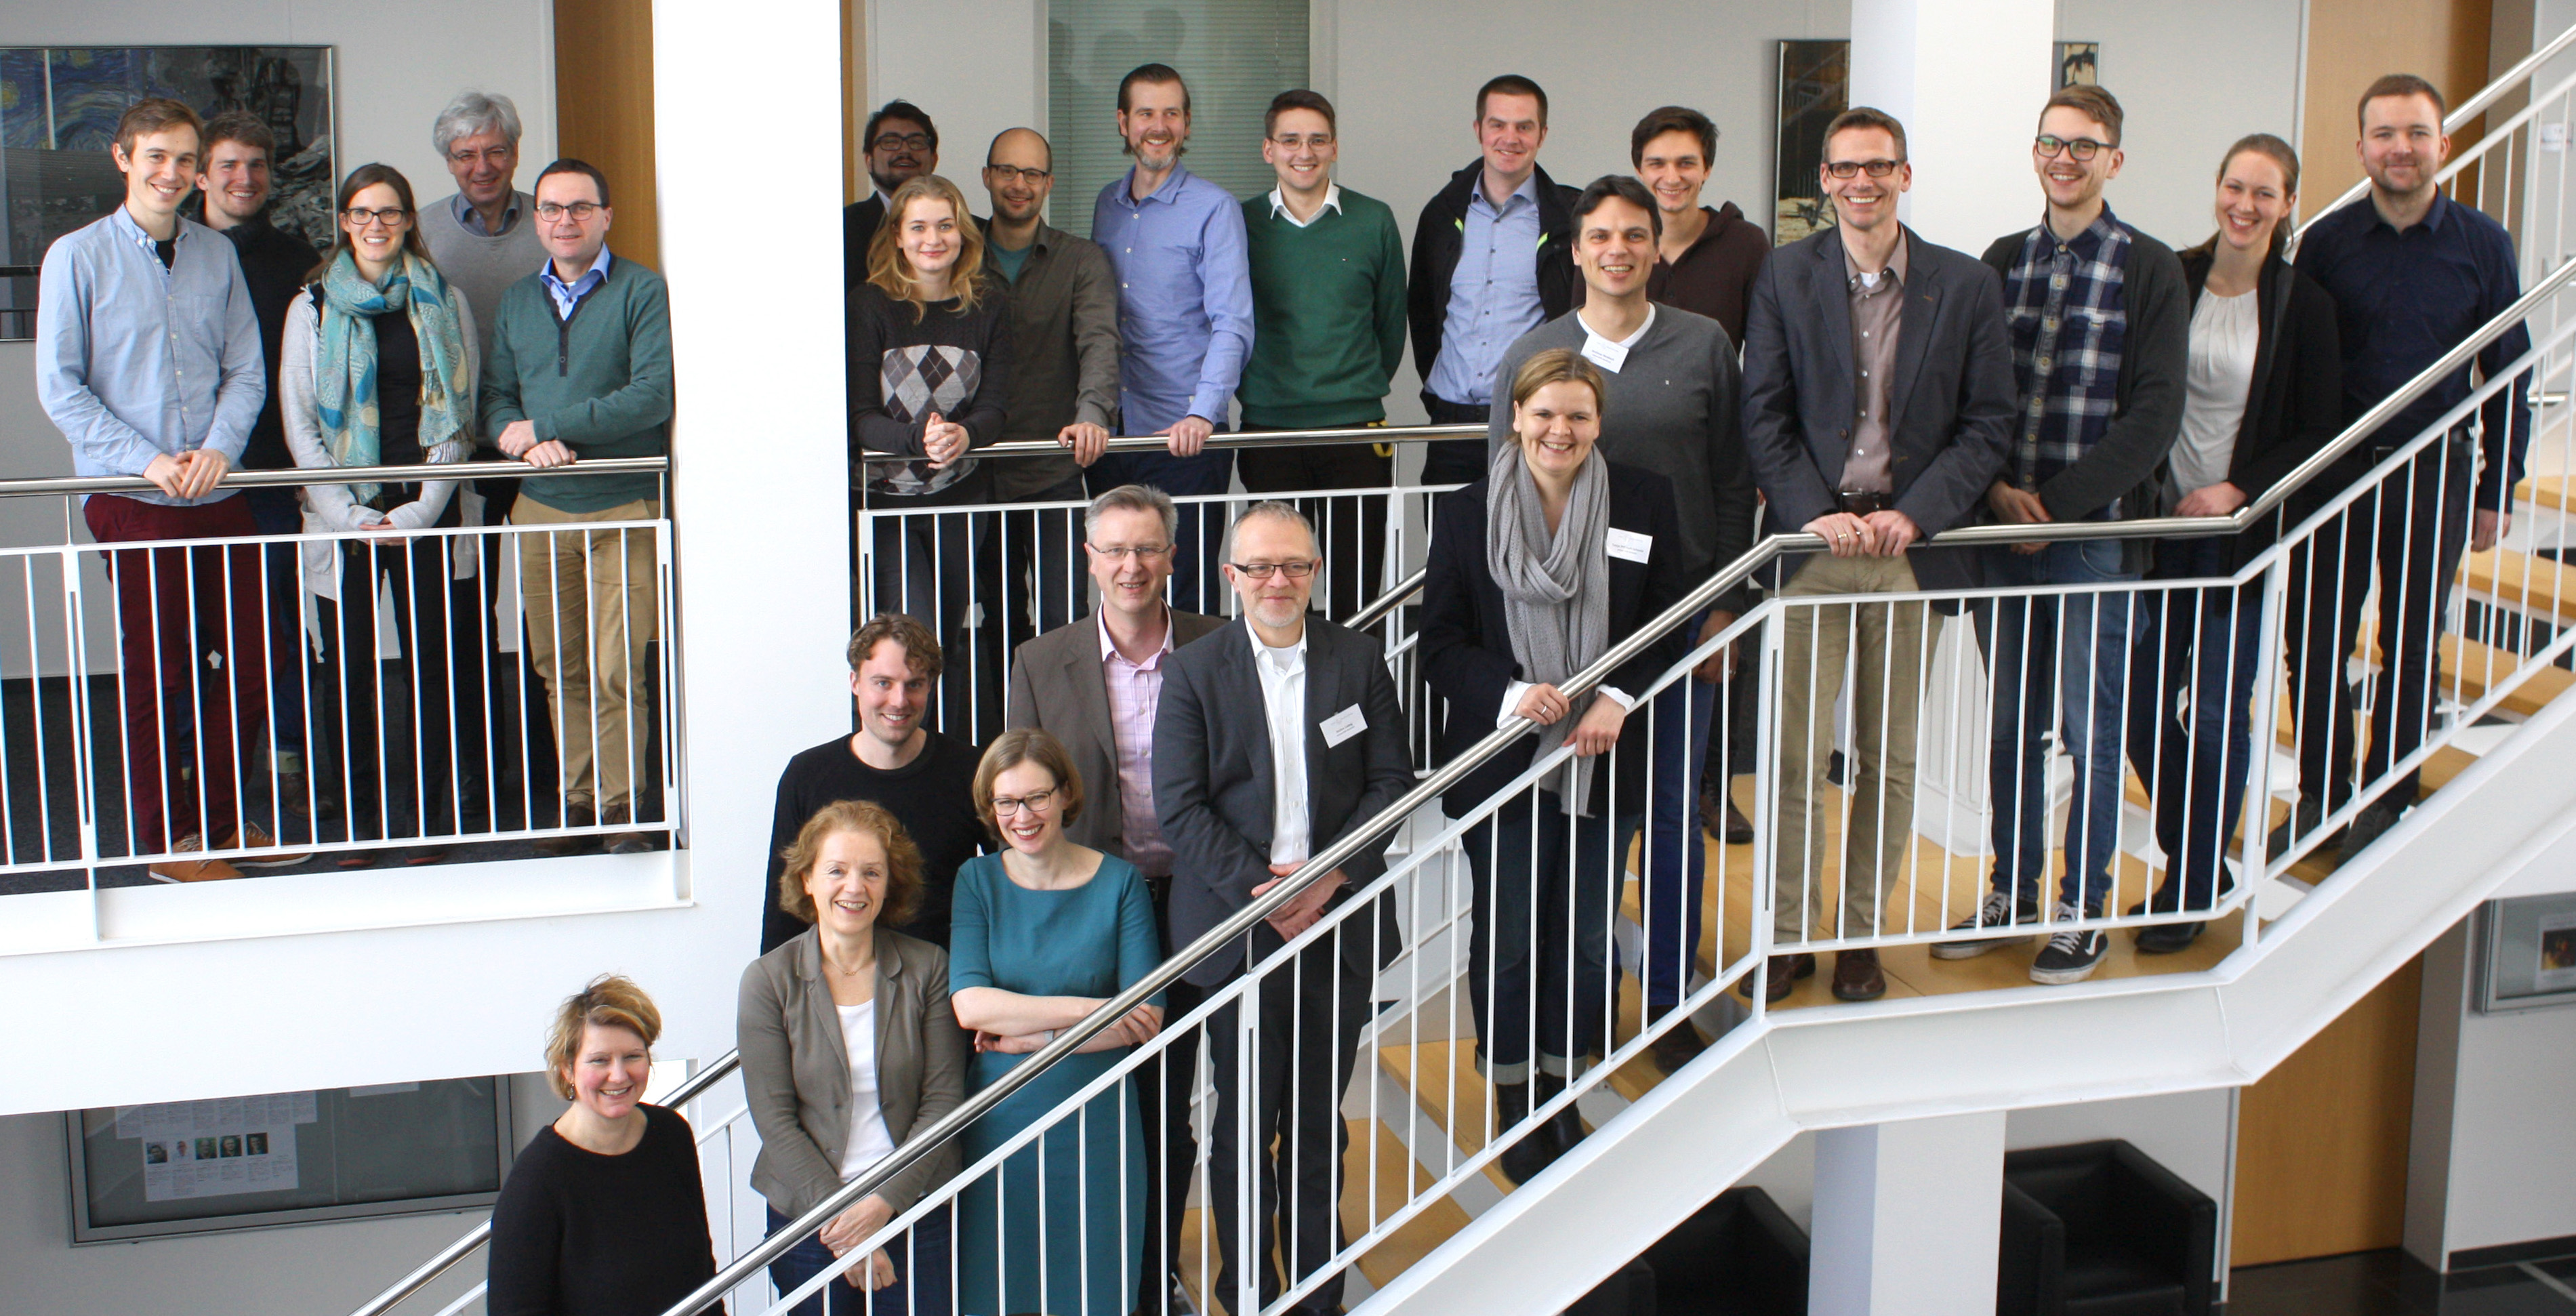
\includegraphics[width=0.8\linewidth]{figures/slides_for.jpg}}
\note{
   \begin{itemize}
      \item Hanse-Wissenschaftskolleg Delmenhorst 2017
   \end{itemize}
}
\end{frame}


%%%%%%%%%%%
% FOLIE 6 %
%%%%%%%%%%%
\begin{frame}{\vspace*{10mm}1\hspace*{1em}Vorgeschichte}
\frame{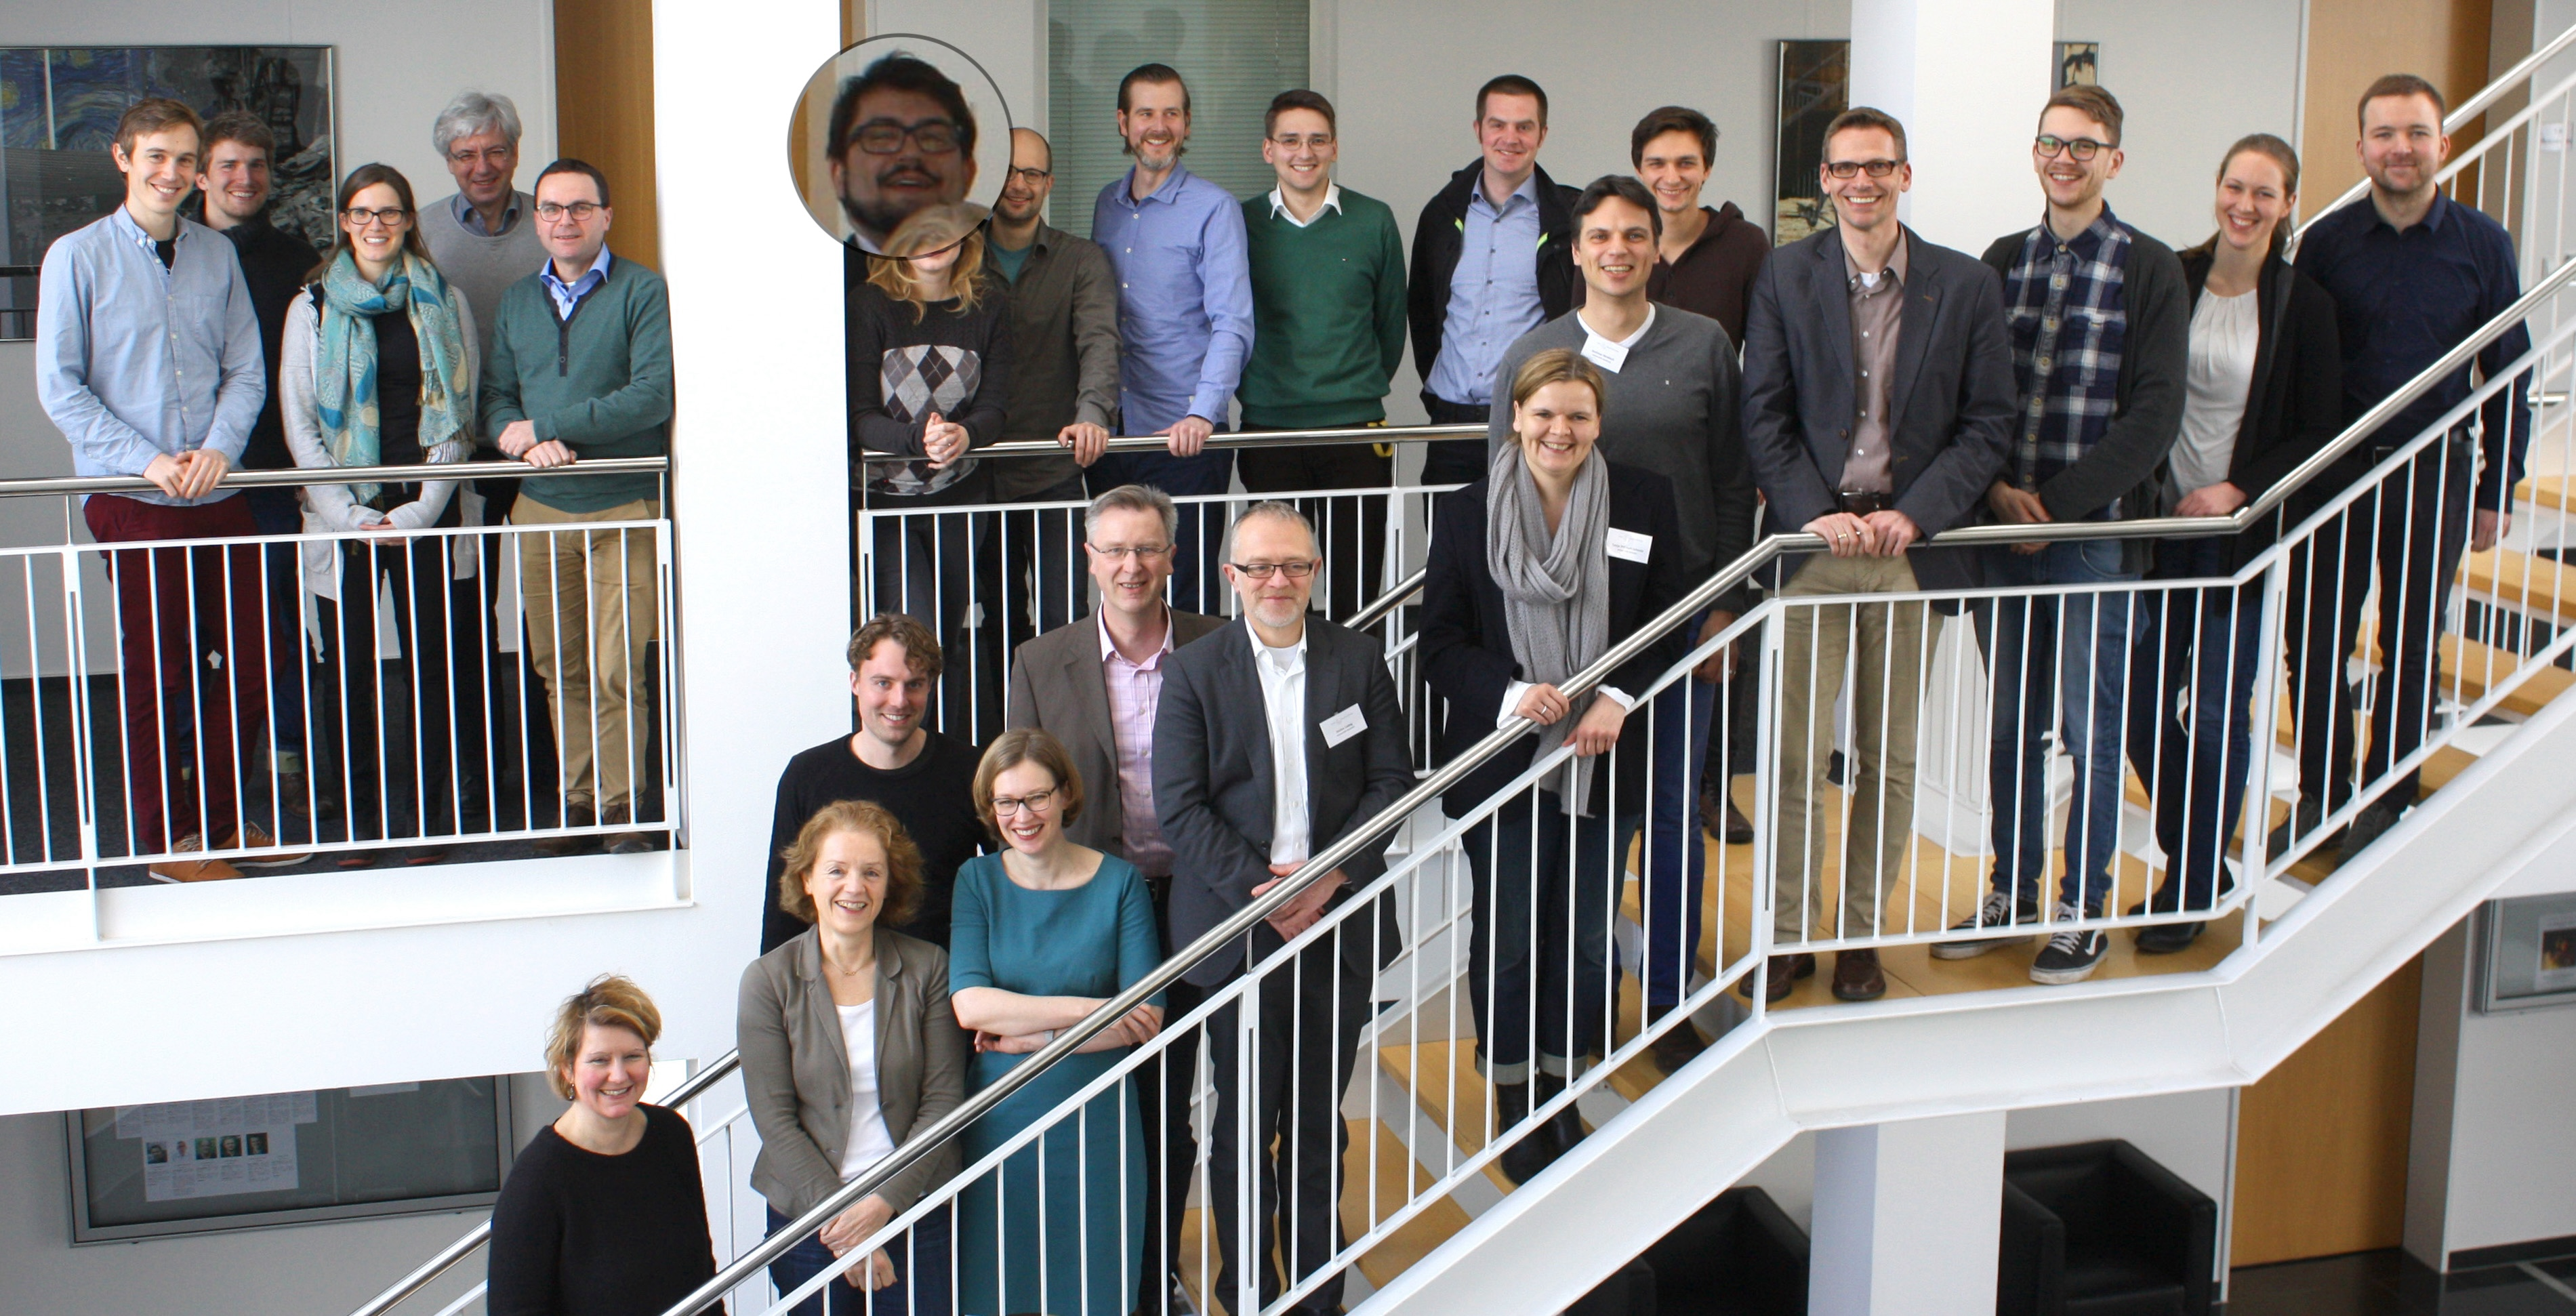
\includegraphics[width=0.8\linewidth]{figures/slides_for_close_up.jpg}}
\end{frame}


%%%%%%%%%%%
% FOLIE 7 %
%%%%%%%%%%%
\begin{frame}
\begin{overlayarea}{\textwidth}{0.81\paperheight}{
   \vspace*{11mm}
   \usebeamerfont{title}\textcolor{uolblue}
   {2\hspace*{1em}Empirische Forschung\\\hspace*{1.5em}und normative Theorie}
}
\end{overlayarea}
\end{frame}


%%%%%%%%%%%
% FOLIE 8 %
%%%%%%%%%%%
\begin{frame}{\vspace*{10mm}2\hspace*{1em}Empirische Forschung und normative Theorie}
\begin{multicols}{2}
   \textbf{Verortung}\\
   \medskip
   \begin{itemize}
      \item Deskriptive Ethik $\in$\\Experimentelle Philosophie
      \item Experimentelle Philosophie $\in$\\Philosophie
   \end{itemize}
   \vfill
   \begin{center}
      \frame{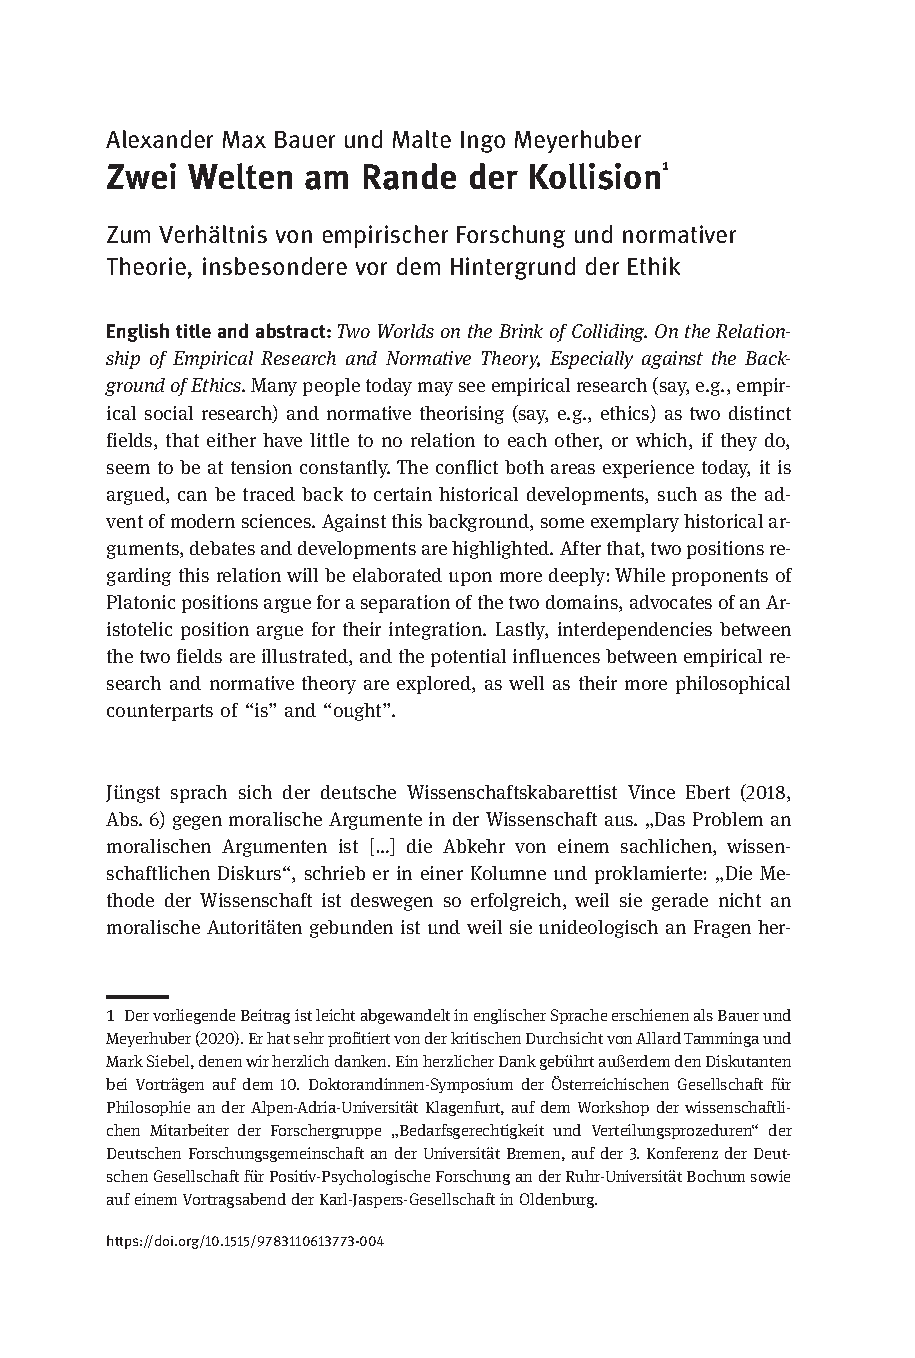
\includegraphics[width=0.6\linewidth]{figures/slides_bauer_meyerhuber_2019.pdf}}\\
      \textcolor{gray}{Bauer und Meyerhuber 2019}
   \end{center}
\end{multicols}
\end{frame}


%%%%%%%%%%%
% FOLIE 9 %
%%%%%%%%%%%
\begin{frame}{\vspace*{10mm}2\hspace*{1em}Empirische Forschung und normative Theorie}
\textbf{Relevanz}\\
\medskip
\begin{itemize}
   \item \enquote{platonische} und \enquote{aristotelische} Perspektive \textcolor{gray}{(Miller 1994, S. 177ff.)}
   \item \enquote{komplementäre Angewiesenheit [\ldots] von empirischer Gerechtigkeitsforschung und normativer Gerechtigkeitstheorie} \textcolor{gray}{(Honneth 2008, S. 10)}
   \item Experimentelle Philosophie kann Beitrag zur Ethik leisten
   \begin{itemize}
      \item Erweiterung der Grundgesamtheit an Introspektionen, die zur Reflexion zur Verfügung stehen
      \item Falsifikation oder Verifikation empirischer Prämissen
      \item Ex-ante- und Ex-post Evaluation der Implementation
   \end{itemize}
\end{itemize}
\note{
   \begin{itemize}
      \item kein naiver Positivismus
   \end{itemize}
}
\end{frame}


%%%%%%%%%%%%
% FOLIE 10 %
%%%%%%%%%%%%
\begin{frame}
\begin{overlayarea}{\textwidth}{0.81\paperheight}{
   \vspace*{11mm}
   \usebeamerfont{title}\textcolor{uolblue}
   {3\hspace*{1em}Bedarf und Bedarfsgerechtigkeit}
}
\end{overlayarea}
\end{frame}


%%%%%%%%%%%%
% FOLIE 11 %
%%%%%%%%%%%%
\begin{frame}{\vspace*{10mm}3\hspace*{1em}Bedarf und Bedarfsgerechtigkeit}
\begin{multicols}{2}
   \textbf{Gerechtigkeit und Verteilungsgerechtigkeit}\\
   \medskip
   \begin{itemize}
      \item \enquote{So hat [\ldots] Simonides nach Dichterart angedeutet, was das Gerechte sei: daß man jedem gebe, was ihm gebühre, und hat dies als Schuldigkeit bezeichnet} \textcolor{gray}{(Platon 2004, S. 13, 332\,b--c)}
      \item \enquote{Von der Gerechtigkeit im speziellen Sinn und dem in ihrem Sinne Gerechten findet sich die eine Form bei der Verteilung von Ehre, Geld oder anderen Gütern, die unter den Mitgliedern der Staatsgemeinschaft teilbar sind} \textcolor{gray}{(Aristoteles 2011, S. 166, 1130\,b)}
   \end{itemize}
   \vfill
   \begin{center}
      \frame{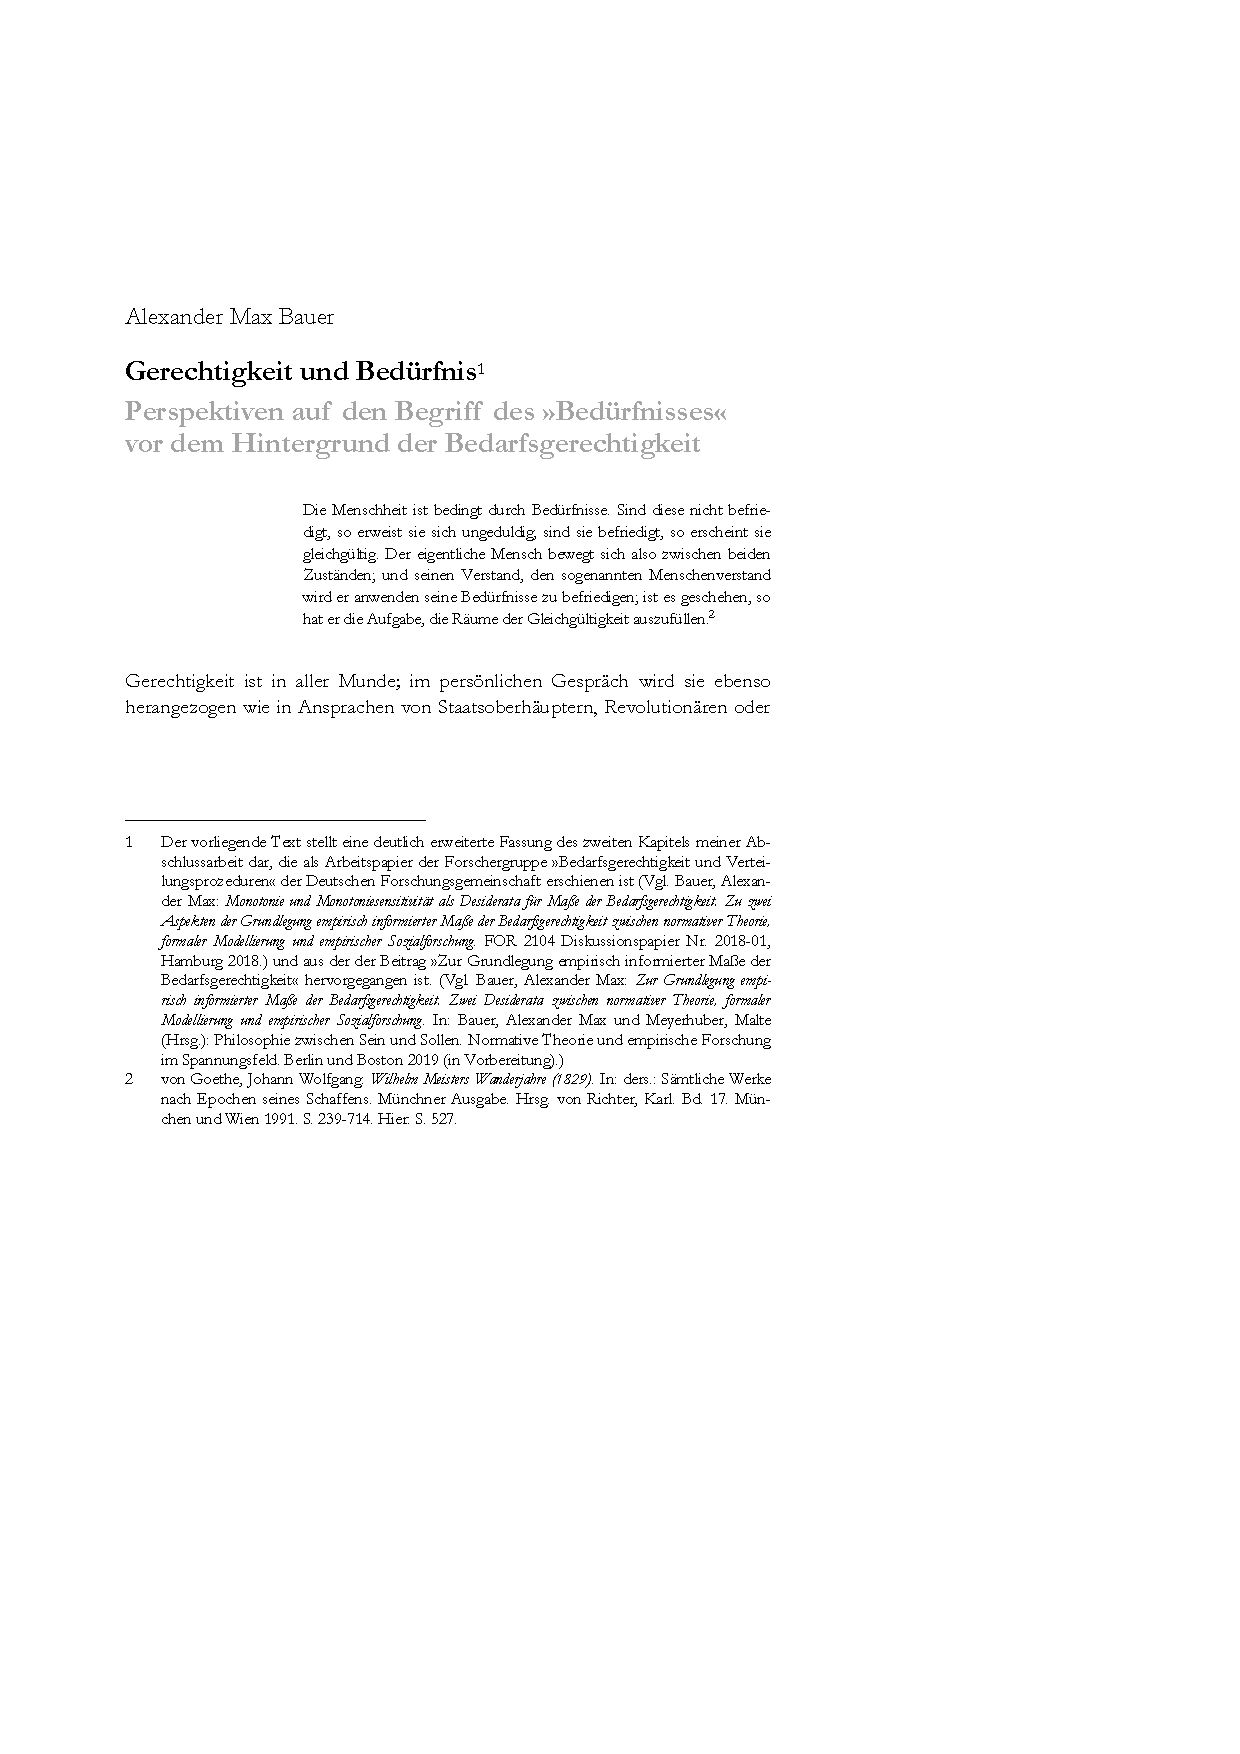
\includegraphics[width=0.6\linewidth]{figures/slides_bauer_2019.pdf}}\\
      \textcolor{gray}{Bauer 2019}
   \end{center}
\end{multicols}
\end{frame}


%%%%%%%%%%%%
% FOLIE 12 %
%%%%%%%%%%%%
\begin{frame}{\vspace*{10mm}3\hspace*{1em}Bedarf und Bedarfsgerechtigkeit}
\textbf{Verteilungsprinzipien}\\
\medskip
\enquote{Stellen Sie sich vor, Sie müssten entscheiden, welches der drei Kinder Anne, Bob und Clara die Flöte haben soll, um die sie sich streiten. Anne verlangt das Instrument für sich, da sie als Einzige von den Dreien Flöte spielen könne [\ldots] und da es ungerecht wäre, die Flöte dem einzigen Kind zu verweigern, das tatsächlich auf ihr spielen kann. [\ldots]\\
\medskip
In einem alternativen Szenario meldet sich Bob und verteidigt seinen Anspruch auf die Flöte mit dem Hinweis, er als Einziger von den Dreien sei so arm, dass er keine eigenen Spielzeuge besitze. Bekäme er die Flöte, hätte er etwas zum Spielen. [\ldots]\\
\medskip
In einem zweiten alternativen Szenario kommt Clara zu Wort und erklärt, dass sie viele Monate lang fleißig gearbeitet habe, um die Flöte selbst zu bauen [\ldots].} \textcolor{gray}{(Sen 2012, S. 41)}\\
\begin{center}
   \begin{tikzpicture}
      \draw[very thick,blue2] (15,0) -- (16.1,0.4);
      \draw[very thick,blue2] (15,0) -- (13.9,0.4);
   \end{tikzpicture}\\
   {\color{blue2} \fontsize{10}{10}\selectfont%
   Für sich genommen legitim erscheinende Verteilungsprinzipien\\[0.2ex]
   können miteinander in Konflikt geraten, wenn sie nicht isoliert betrachtet werden}
\end{center}
\note{
   \begin{itemize}
      \item Prinzipienmonismus
      \item Prinzipienpluralismus
      \begin{itemize}
         \item Rangfolge (Rawls)
         \item Kontextabhängigkeit (Walzer)
      \end{itemize}
   \end{itemize}
}
\end{frame}


%%%%%%%%%%%%
% FOLIE 13 %
%%%%%%%%%%%%
\begin{frame}{\vspace*{10mm}3\hspace*{1em}Bedarf und Bedarfsgerechtigkeit}
\textbf{Bedarfsprinzip}\\
\medskip
\begin{itemize}
   \item Wer (Umfang) soll wieviel (Form) wovon (Gut) erhalten? \textcolor{gray}{(Page 2006, Siebel und Schramme 2020)}
   \item Bedürftige sollen das, dessen sie bedürfen, in vollem Umfang erhalten
   \begin{itemize}
      \item Wie verteilt man Ressourcen, wenn weniger oder mehr zur Verfügung steht, als insgesamt gebraucht wird?
      \item Wann lässt sich sagen, dass jemand etwas bedarf?
   \end{itemize}
\end{itemize}
\note{
   \begin{itemize}
      \item Klassifikation von Verteilungsprinzipien
   \end{itemize}
}
\end{frame}


%%%%%%%%%%%%
% FOLIE 14 %
%%%%%%%%%%%%
\begin{frame}{\vspace*{10mm}3\hspace*{1em}Bedarf und Bedarfsgerechtigkeit}
\textbf{Bedarf}\\
\medskip
\begin{itemize}
   \item \enquote{$S$ benötigt $X$, um $Z$ in $U$ zu erreichen} \textcolor{gray}{(nach Siebel und Schramme 2020, S. 27)}
   \item Unterscheidung zwischen bloß instrumentellen und fundamentalen Bedürfnissen (z.\,B. durch Ermöglichung würdevoller Lebensumstände oder Vermeidung von Schaden)
   \item Abgrenzung von bloßen Präferenzen und Wünschen (z.\,B. durch intersubjektive Anerkennung)
\end{itemize}
\end{frame}


%%%%%%%%%%%%
% FOLIE 15 %
%%%%%%%%%%%%
\begin{frame}
\begin{overlayarea}{\textwidth}{0.81\paperheight}{
   \vspace*{11mm}
   \usebeamerfont{title}\textcolor{uolblue}
   {4\hspace*{1em}Bedarf als Referenzpunkt}
}
\end{overlayarea}
\end{frame}


%%%%%%%%%%%%
% FOLIE 16 %
%%%%%%%%%%%%
\begin{frame}{\vspace*{10mm}4\hspace*{1em}Bedarf als Referenzpunkt}
\begin{multicols}{2}
   \textbf{Hintergrund}\\
   \medskip
   \begin{itemize}
      \item Menschen nehmen graduelle Gerechtigkeitseinschätzungen von Verteilungssituationen vor
      \item Gibt es einen Zusammenhang zwischen Gerechtigkeitseinschätzung und Bedarfsdeckung? Welche Rolle spielt dabei eine Bedarfsschwelle?
   \end{itemize}
   \vfill
   \begin{center}
      \frame{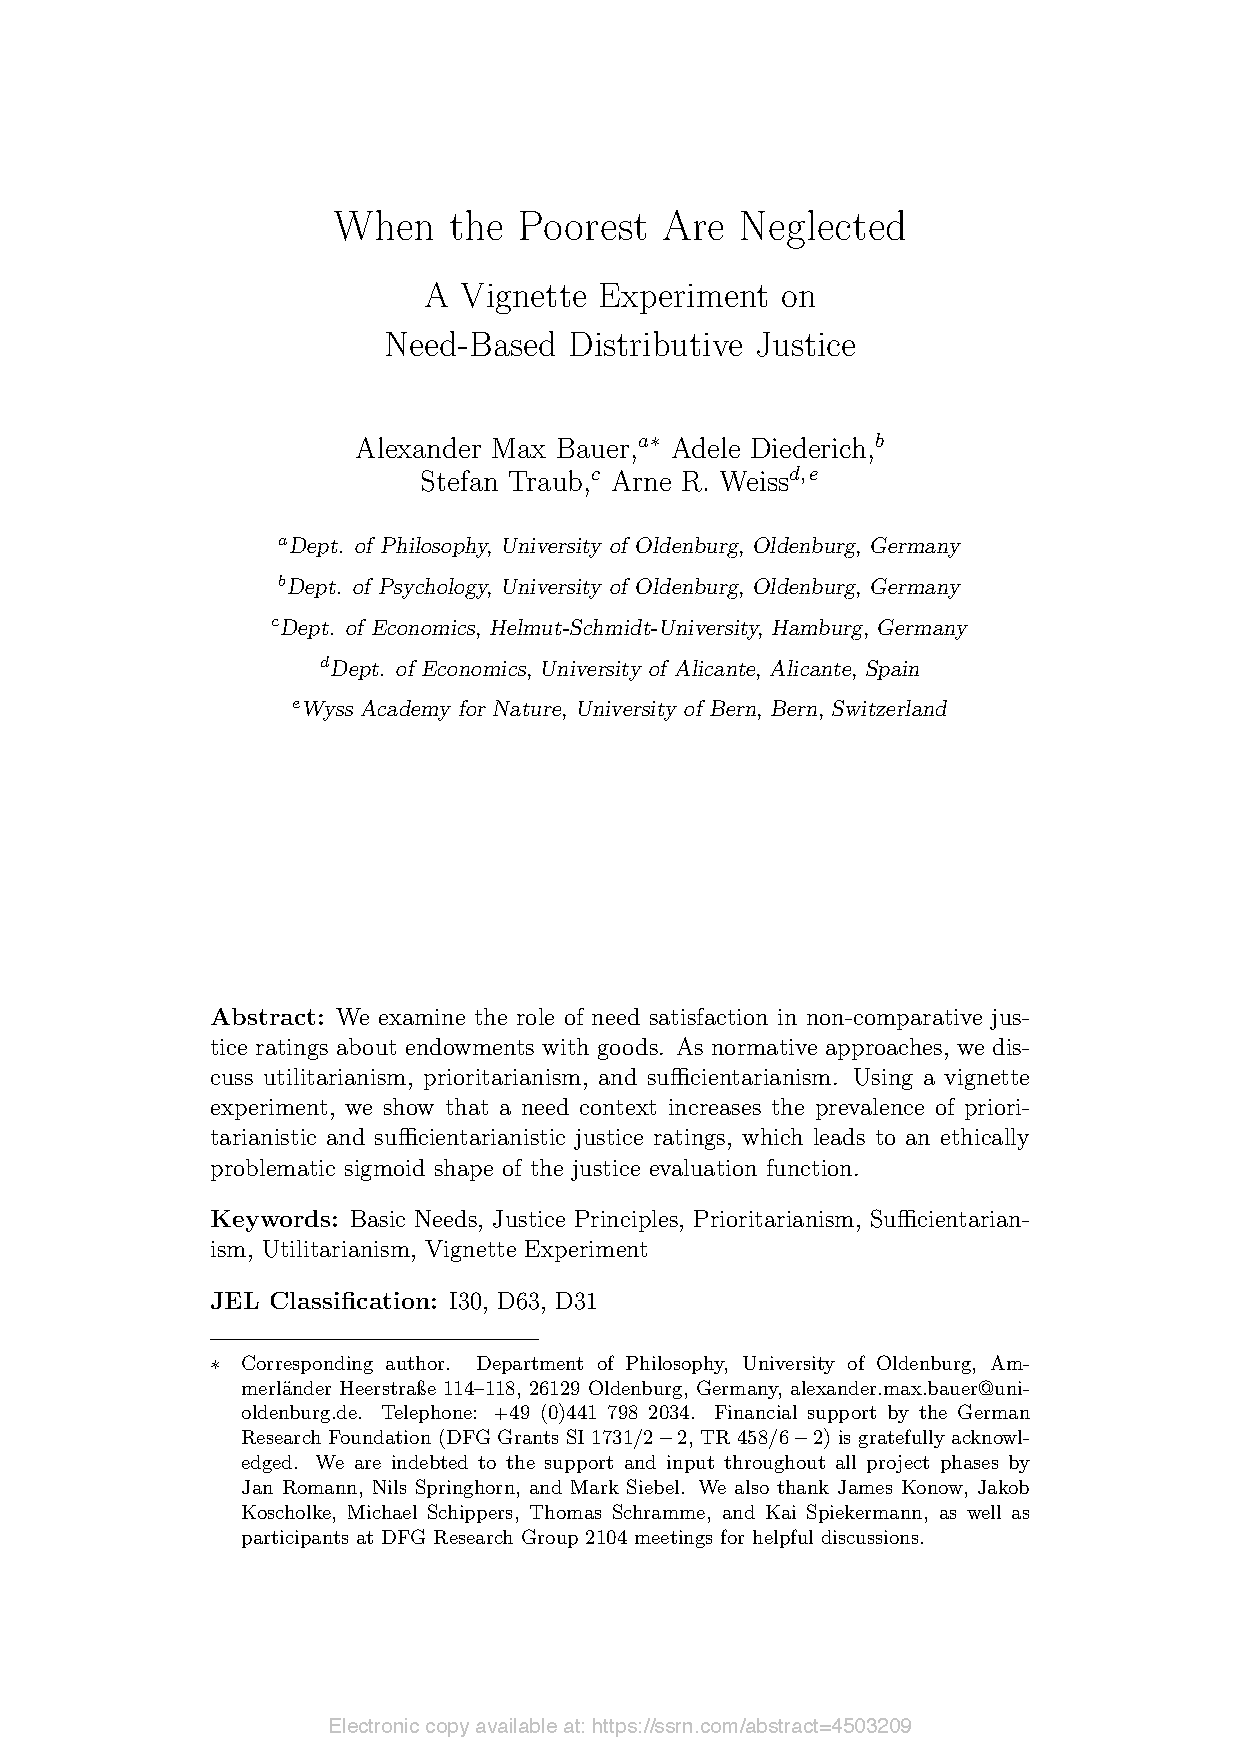
\includegraphics[width=0.6\linewidth]{figures/slides_bauer_et_al_2023a.pdf}}\\
      \textcolor{gray}{Bauer et al. 2023a}
   \end{center}
\end{multicols}
\end{frame}


%%%%%%%%%%%%
% FOLIE 17 %
%%%%%%%%%%%%
\begin{frame}{\vspace*{10mm}4\hspace*{1em}Bedarf als Referenzpunkt}
\textbf{Design und Durchführung}\\
\medskip
\begin{itemize}
   \item WiSo-Experimentallabor, Universität Hamburg, September 2016
   \item $n=116$
   \item Unparteiische Beobachter*innen
   \item Bedarfs- und Kontrollgruppe (\textit{between subjects})
   \item Globale und relative Einschätzungsaufgabe (\textit{within subjects})
   \item $11$ Verteilungssituationen, eingebettet in hypothetischen Kontext
\end{itemize}
\end{frame}


%%%%%%%%%%%%
% FOLIE 18 %
%%%%%%%%%%%%
\begin{frame}{\vspace*{10mm}4\hspace*{1em}Bedarf als Referenzpunkt}
\textbf{Vignette (1/2)}\\
\medskip
\enquote{Bitte stellen Sie sich Folgendes vor:\\
\medskip
In der Region Bergtal soll das neue Dorf Ahdorf gegründet werden. Der dortige Bau von Wohnraum ist Aufgabe der öffentlichen Wohnungsbaugesellschaft von Bergtal.\\
\medskip
Alle Haushalte in dieser Region möchten in möglichst großem Wohnraum leben. Die Bewohner der Region haben sich gemeinsam auf Untergrenzen an Wohnraum verständigt, unterhalb derer ein würdevolles Leben in dieser Gesellschaft nicht möglich ist. Zwischen den Haushalten in dieser Region gibt es keine nennenswerten Unterschiede und die Untergrenzen sind für jeden Haushalt gleich: Jeder Haushalt sollte mindestens über 1.000 regionale -- also in dieser Region gebräuchliche -- Größeneinheiten an Wohnraum verfügen, um ein würdevolles Leben führen zu können. Ein Wohnraum der entsprechenden Größe bedeutet für einen Haushalt zwar ein Leben in beengten Verhältnissen, genügt aber gerade noch, um ein würdevolles Leben führen zu können.}
\end{frame}


%%%%%%%%%%%%
% FOLIE 19 %
%%%%%%%%%%%%
\begin{frame}{\vspace*{10mm}4\hspace*{1em}Bedarf als Referenzpunkt}
\textbf{Vignette (2/2)}\\
\medskip
\enquote{Es sind ausreichend Mittel vorhanden, um für jeden Haushalt bis zu $2.000$ regionale Größeneinheiten an Wohnraum bauen zu können. Das Regionalparlament entscheidet, wie viel Wohnraum für die Bewohner des neuen Dorfes tatsächlich gebaut wird. Die Entscheidung hat ansonsten keine nennenswerten Auswirkungen.\\
\medskip
Für den Bau von Wohnraum würde keine zusätzliche Fläche verbraucht. Das neue Dorf soll auf der Fläche eines verlassenen Dorfes gegründet werden, das verlassen wurde, nachdem ein Brand die Häuser zerstört hatte.\\
\medskip
Bei seiner Entscheidung will das Regionalparlament berücksichtigen, wie gerecht die Szenarien von unabhängigen Personen -- wie Ihnen -- beurteilt werden. Ihre Aufgabe ist daher, für jedes Szenario anzugeben, für wie gerecht Sie die Verteilung von Wohnraum jeweils halten.}
\end{frame}


%%%%%%%%%%%%
% FOLIE 20 %
%%%%%%%%%%%%
\begin{frame}{\vspace*{10mm}4\hspace*{1em}Bedarf als Referenzpunkt}
\textbf{Abfrage (1/2)}\\
\medskip
\begin{center}
   \frame{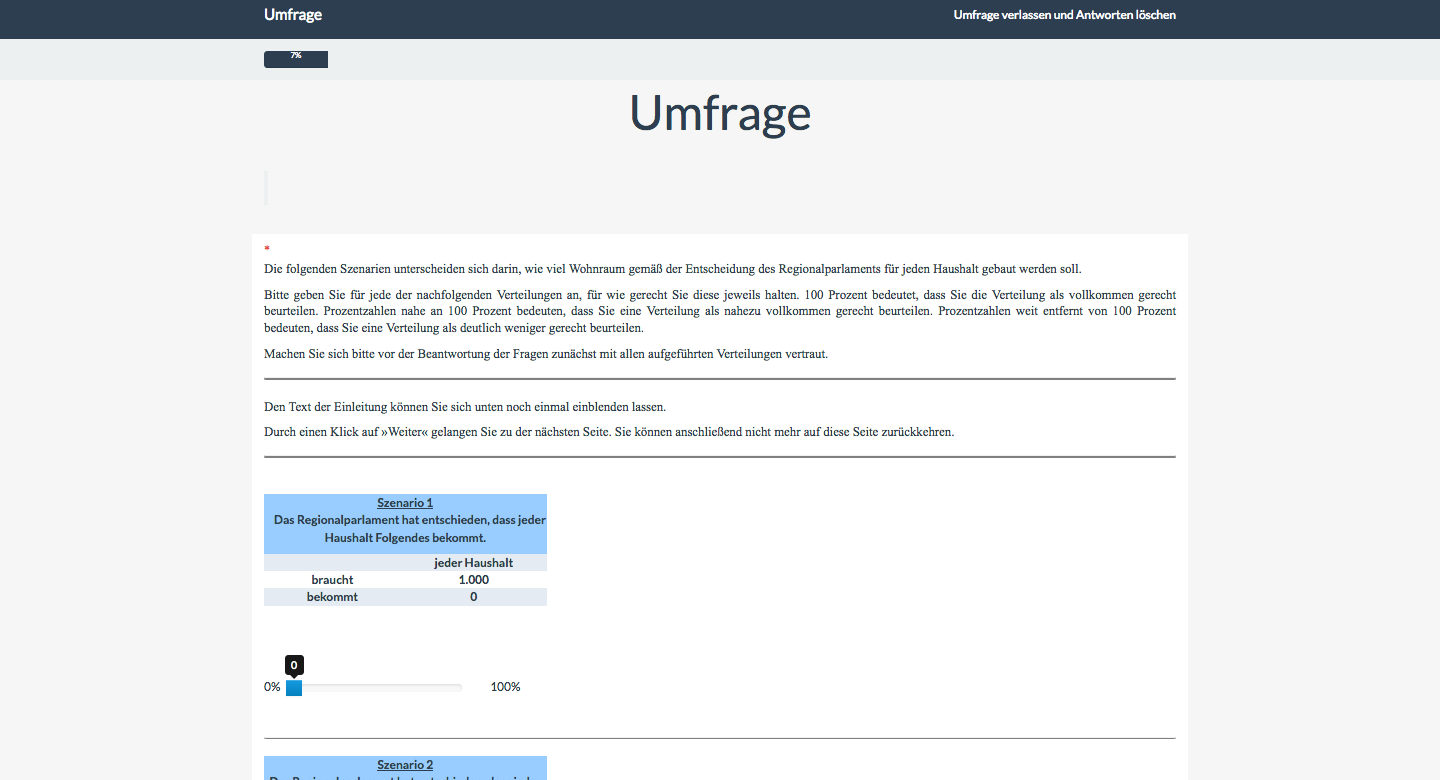
\includegraphics[width=0.5\linewidth]{figures/slides_lime_1.png}}\\
   \textcolor{gray}{Globale Einschätzungsaufgabe}
\end{center}
\end{frame}


%%%%%%%%%%%%
% FOLIE 21 %
%%%%%%%%%%%%
\begin{frame}{\vspace*{10mm}4\hspace*{1em}Bedarf als Referenzpunkt}
\textbf{Abfrage (2/2)}\\
\begin{multicols}{2}
   \begin{center}
      \frame{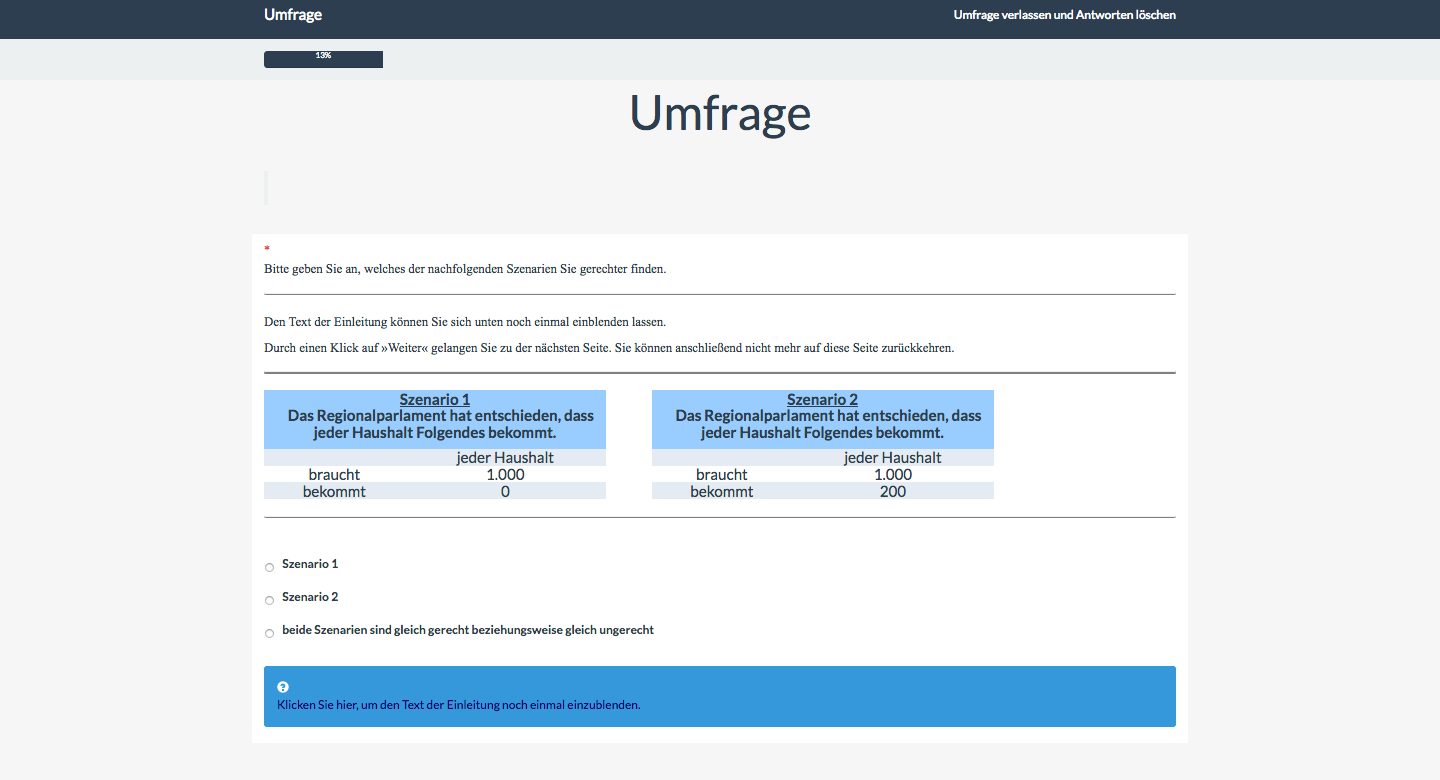
\includegraphics[width=1\linewidth]{figures/slides_lime_2.png}}\\
      \textcolor{gray}{Relative Einschätzungsaufgabe, Teil 1}
      \frame{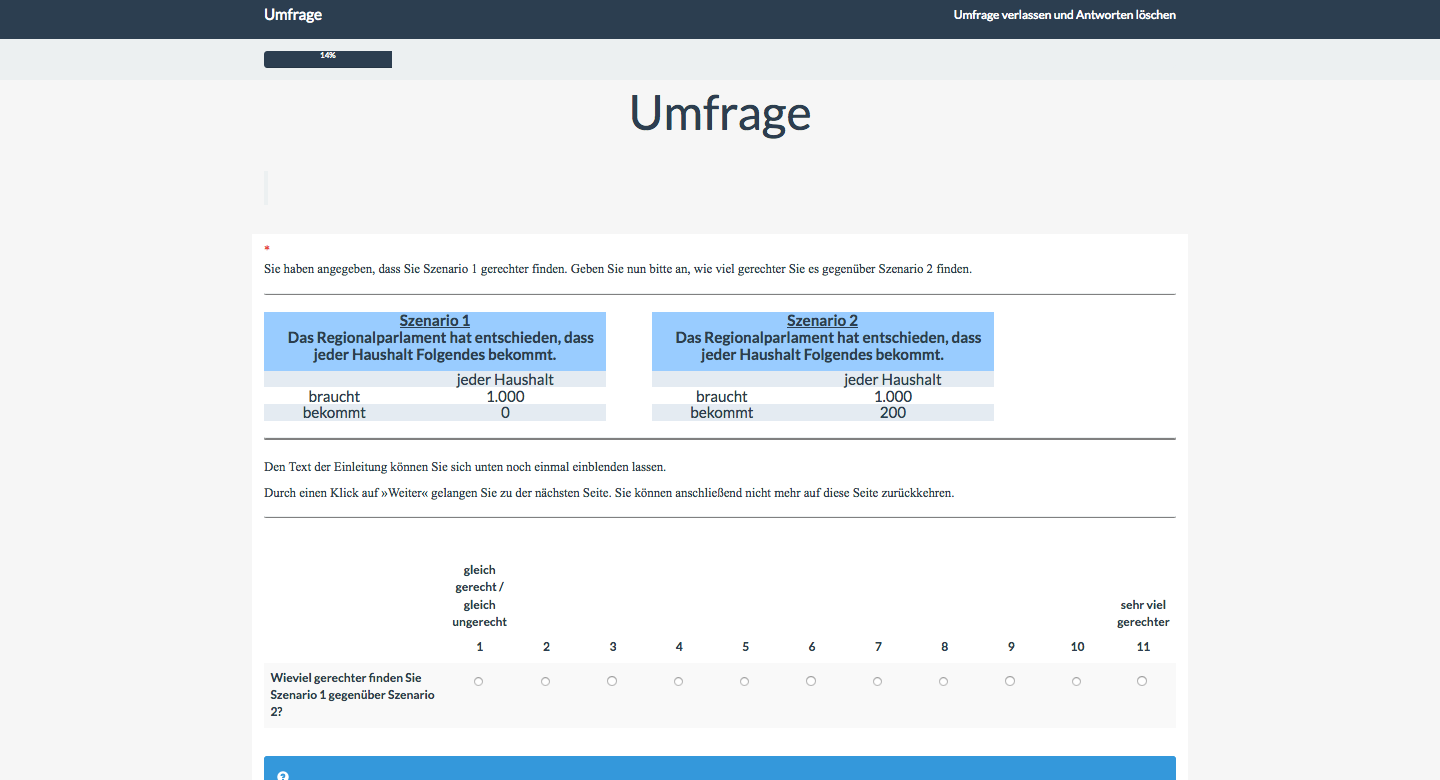
\includegraphics[width=1\linewidth]{figures/slides_lime_3.png}}\\
      \textcolor{gray}{Relative Einschätzungsaufgabe, Teil 2}
   \end{center}
\end{multicols}
\end{frame}


%%%%%%%%%%%%
% FOLIE 22 %
%%%%%%%%%%%%
\begin{frame}{\vspace*{10mm}4\hspace*{1em}Bedarf als Referenzpunkt}
\textbf{Ergebnisse (1/2)}\\
\begin{multicols}{2}
   \begin{center}
      \frame{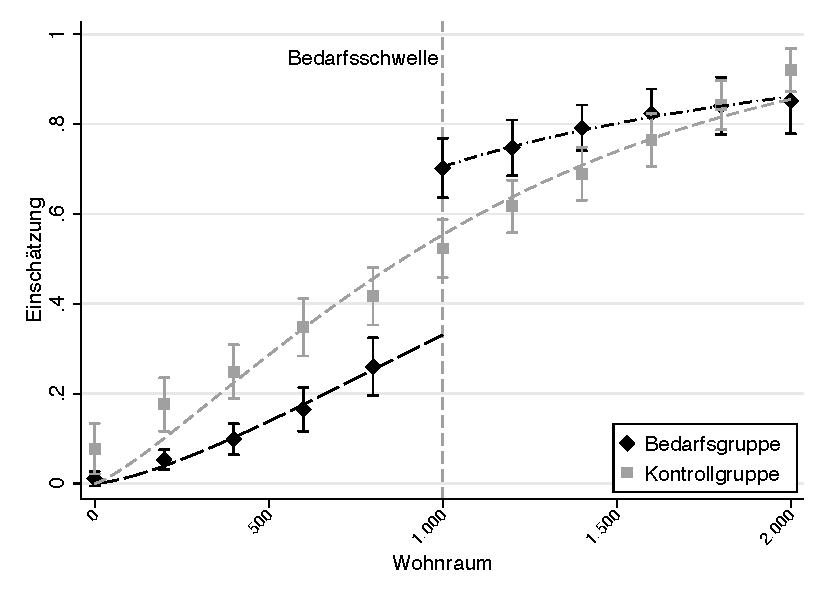
\includegraphics[width=1\linewidth]{figures/figure_1.pdf}}\\
      \textcolor{gray}{Globale Einschätzungsaufgabe}
      \frame{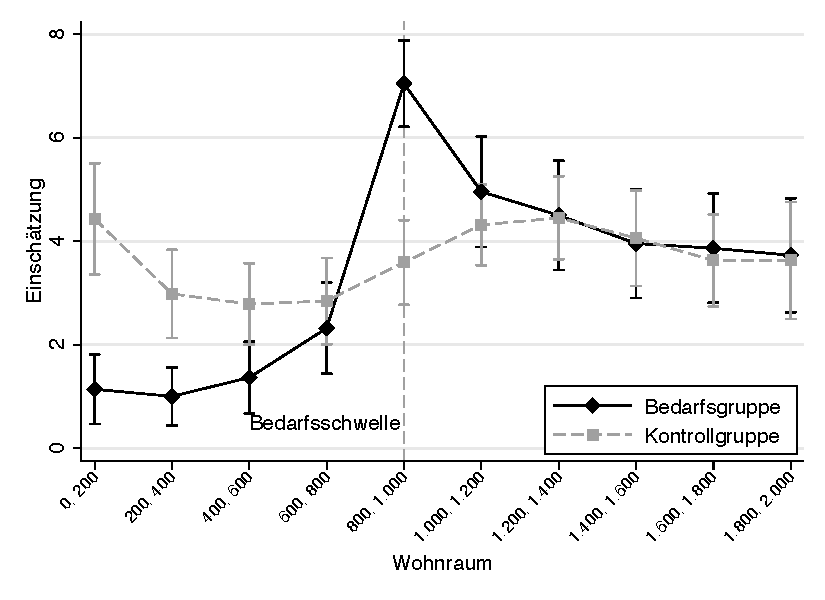
\includegraphics[width=1\linewidth]{figures/figure_2.pdf}}\\
      \textcolor{gray}{Relative Einschätzungsaufgabe}
   \end{center}
\end{multicols}
\note{
   \begin{itemize}
      \item Globale Einschätzungsaufgabe
      \begin{itemize}
         \item Weibul-Schätzung (Referenzpunkte bei $0$ und $1.000$ Einheiten)
         \item Sprunghafter Anstieg (etwa $35$ Prozentpunkte), unterhalb der Schwelle konvex, oberhalb konkav
         \item Einschätzungen unterhalb der Schwelle (mit Ausnahme von $0$ Einheiten) in Bedarfsgruppe signifikant niedriger
         \item Einschätzungen oberhalb der Schwelle (mit Ausnahme von $1.600$, $1,800$ und $2.000$ Einheiten) in Bedarfsgruppe signifikant höher
      \end{itemize}
      \item Relative Einschätzungsaufgabe
      \begin{itemize}
         \item Vergleiche in Kontrollgruppe mäandern um $3$ und $4$ Punkte
         \item Einschätzungen unterhalb der Schwelle (mit Ausnahme von $600$, $800$ Einheiten) in Bedarfsgruppe signifikant niedriger
         \item Einschätzungen bei Erreichen der Schwelle in Bedarfsgruppe signifikant höher
      \end{itemize}
   \end{itemize}
}
\end{frame}


%%%%%%%%%%%%
% FOLIE 23 %
%%%%%%%%%%%%
\begin{frame}{\vspace*{10mm}4\hspace*{1em}Bedarf als Referenzpunkt}
\textbf{Ergebnisse (2/2)}\\
\medskip
\begin{itemize}
   \item Unparteiische Beobachter*innen nehmen graduelle Gerechtigkeitseinschätzungen vor
   \item Einschätzungen abhängig von Versorgungssituation
   \item Bedarfsinformationen beeinflussen Einschätzungen
\end{itemize}
\end{frame}


%%%%%%%%%%%%
% FOLIE 24 %
%%%%%%%%%%%%
\begin{frame}
\begin{overlayarea}{\textwidth}{0.81\paperheight}{
   \vspace*{11mm}
   \usebeamerfont{title}\textcolor{uolblue}
   {5\hspace*{1em}Bedarf und Verantwortung}
}
\end{overlayarea}
\end{frame}


%%%%%%%%%%%%
% FOLIE 25 %
%%%%%%%%%%%%
\begin{frame}{\vspace*{10mm}5\hspace*{1em}Bedarf und Verantwortung}
\begin{multicols}{2}
   \textbf{Hintergrund}\\
   \medskip
   \begin{itemize}
      \item Menschen berücksichtigen verschiedene (normativ relevante) Faktoren, wenn sie Verteilungsentscheidungen treffen
      \item Welche Rolle spielen Unterschiede in Produktivität, Bedarf und Verantwortung bei unparteiischen Verteilungsentscheidungen?
   \end{itemize}
   \vfill
   \begin{center}
      \frame{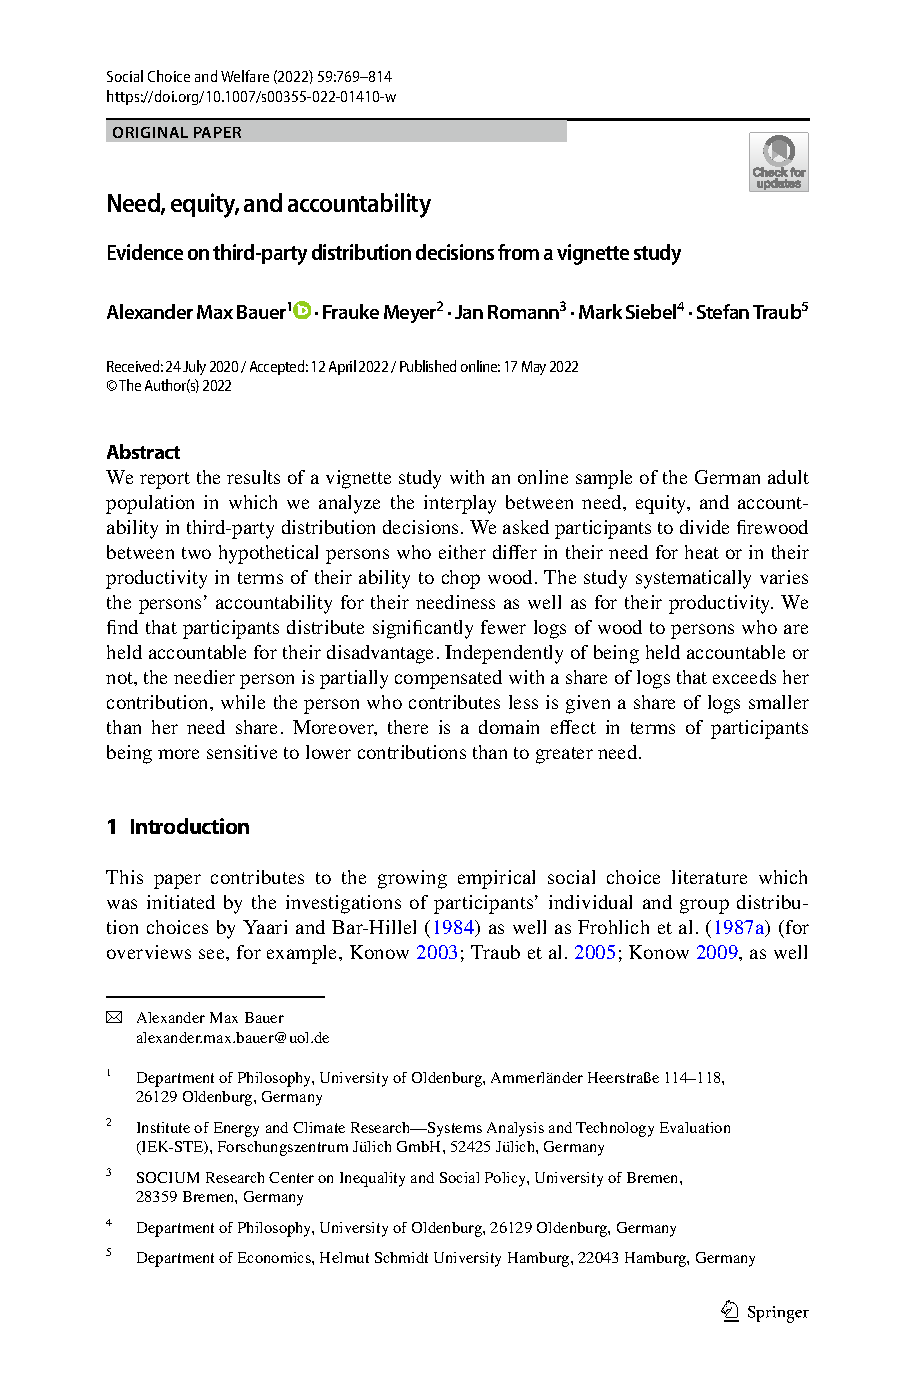
\includegraphics[width=0.6\linewidth]{figures/slides_bauer_et_al_2022.pdf}}\\
      \textcolor{gray}{Bauer et al. 2022}
   \end{center}
\end{multicols}
\end{frame}


%%%%%%%%%%%%
% FOLIE 26 %
%%%%%%%%%%%%
\begin{frame}{\vspace*{10mm}5\hspace*{1em}Bedarf und Verantwortung}
\textbf{Design und Durchführung (1/2)}\\
\medskip
\begin{itemize}
   \item Respondi, Online-Panel, September 2019
   \item $n=200$ (stratifiziert nach Geschlecht, Alter und Haushaltsäquivalenznettoeinkommen)
   \item Unparteiische Entscheider*innen
   \item Verantwortlichkeits- und Nichtverantwortlichkeitsgruppe (\textit{between subjects})
   \item Bedarfs- und Produktivitätsszenario (\textit{within subjects})
   \item $10$ Verteilungsaufgaben, eingebettet in hypothetischen Kontext
\end{itemize}
\end{frame}


%%%%%%%%%%%%
% FOLIE 27 %
%%%%%%%%%%%%
\begin{frame}{\vspace*{10mm}5\hspace*{1em}Bedarf und Verantwortung}
\textbf{Design und Durchführung (2/2)}\\
\medskip
\begin{center}
   \begin{tabular}{lrrrrr}
      \arrayrulecolor{blue2}
      \hline
      Fall                      & \multicolumn{1}{c}{1}     & \multicolumn{1}{c}{2}     & \multicolumn{1}{c}{3}     & \multicolumn{1}{c}{4}   & \multicolumn{1}{c}{5}       \\
      \hline\hline\\[-0.5em]
                                & \multicolumn{5}{c}{Bedarfsszenario}                                                                                                       \\[0.5em]
      Bedarf A                  &                  1.800    &                  1.400    &                  1.000    &                    700    &                    600    \\
      Produktivität A           & \textcolor{gray}{1.000}   & \textcolor{gray}{1.000}   & \textcolor{gray}{1.000}   & \textcolor{gray}{1.000}   & \textcolor{gray}{1.000}   \\[0.5em]
      Bedarf B                  &                  1.200    &                    800    &                    400    &                    200    &                    100    \\
      Produktivität B           & \textcolor{gray}{1.000}   & \textcolor{gray}{1.000}   & \textcolor{gray}{1.000}   & \textcolor{gray}{1.000}   & \textcolor{gray}{1.000}   \\
      \hline
                                & \multicolumn{5}{c}{Produktivitätsszenario}                                                                                                \\[0.5em]
      Bedarf A                  & \textcolor{gray}{1.000}   & \textcolor{gray}{1.000}   & \textcolor{gray}{1.000}   & \textcolor{gray}{1.000}   & \textcolor{gray}{1.000}   \\
      Produktivität A           &                  1.200    &                    800    &                    400    &                    200    &                    100    \\[0.5em]
      Bedarf B                  & \textcolor{gray}{1.000}   & \textcolor{gray}{1.000}   & \textcolor{gray}{1.000}   & \textcolor{gray}{1.000}   & \textcolor{gray}{1.000}   \\
      Produktivität B           &                  1.800    &                  1.400    &                  1.000    &                    700    &                    600    \\
      \hline
   \end{tabular}\\
   \smallskip
   \textcolor{gray}{Parametrisierung}
\end{center}
\end{frame}


%%%%%%%%%%%%
% FOLIE 28 %
%%%%%%%%%%%%
\begin{frame}{\vspace*{10mm}5\hspace*{1em}Bedarf und Verantwortung}
\textbf{Vignette (Verantwortlichkeitsgruppe, Produktivitätsszenario)}\\
\medskip
\enquote{Bitte stellen Sie sich zwei Personen, \textit{Person~A} und \textit{Person~B} vor, die sich nicht kennen. Beide heizen ausschließlich mit Holz und haben genug Holz auf Lager, um im Winter zu überleben.\\
\medskip
Jedoch benötigen sie zusätzliches Holz, um im Winter nicht zu frieren. Die zuständige Gemeinde ermöglicht den beiden Personen, in einem bestimmten Zeitraum im gemeindeeigenen Wald für den kommenden Winter Holz zu schlagen. \textit{Person~A} und \textit{Person~B} verfügen über wenig Geld und haben daher keine andere Möglichkeit, sich Holz zu besorgen.\\
\medskip
\textit{Person~A} und \textit{Person~B} brauchen beide jeweils $X$ Holzscheite.\\
\medskip
\textit{Person~A} hat $Y$ und \textit{Person~B} hat $Z$ Holzscheite geschlagen.\\
\medskip
\textit{Person~A} hat gegen den Rat seines Arztes weiterhin stark geraucht und leidet daher nun an einer Herz-Kreislaufkrankheit. Deswegen hat \textit{Person~A} weniger Holz geschlagen als \textit{Person~B}.}
\end{frame}


%%%%%%%%%%%%
% FOLIE 29 %
%%%%%%%%%%%%
\begin{frame}{\vspace*{10mm}5\hspace*{1em}Bedarf und Verantwortung}
\textbf{Abfrage}\\
\medskip
\begin{center}
   \frame{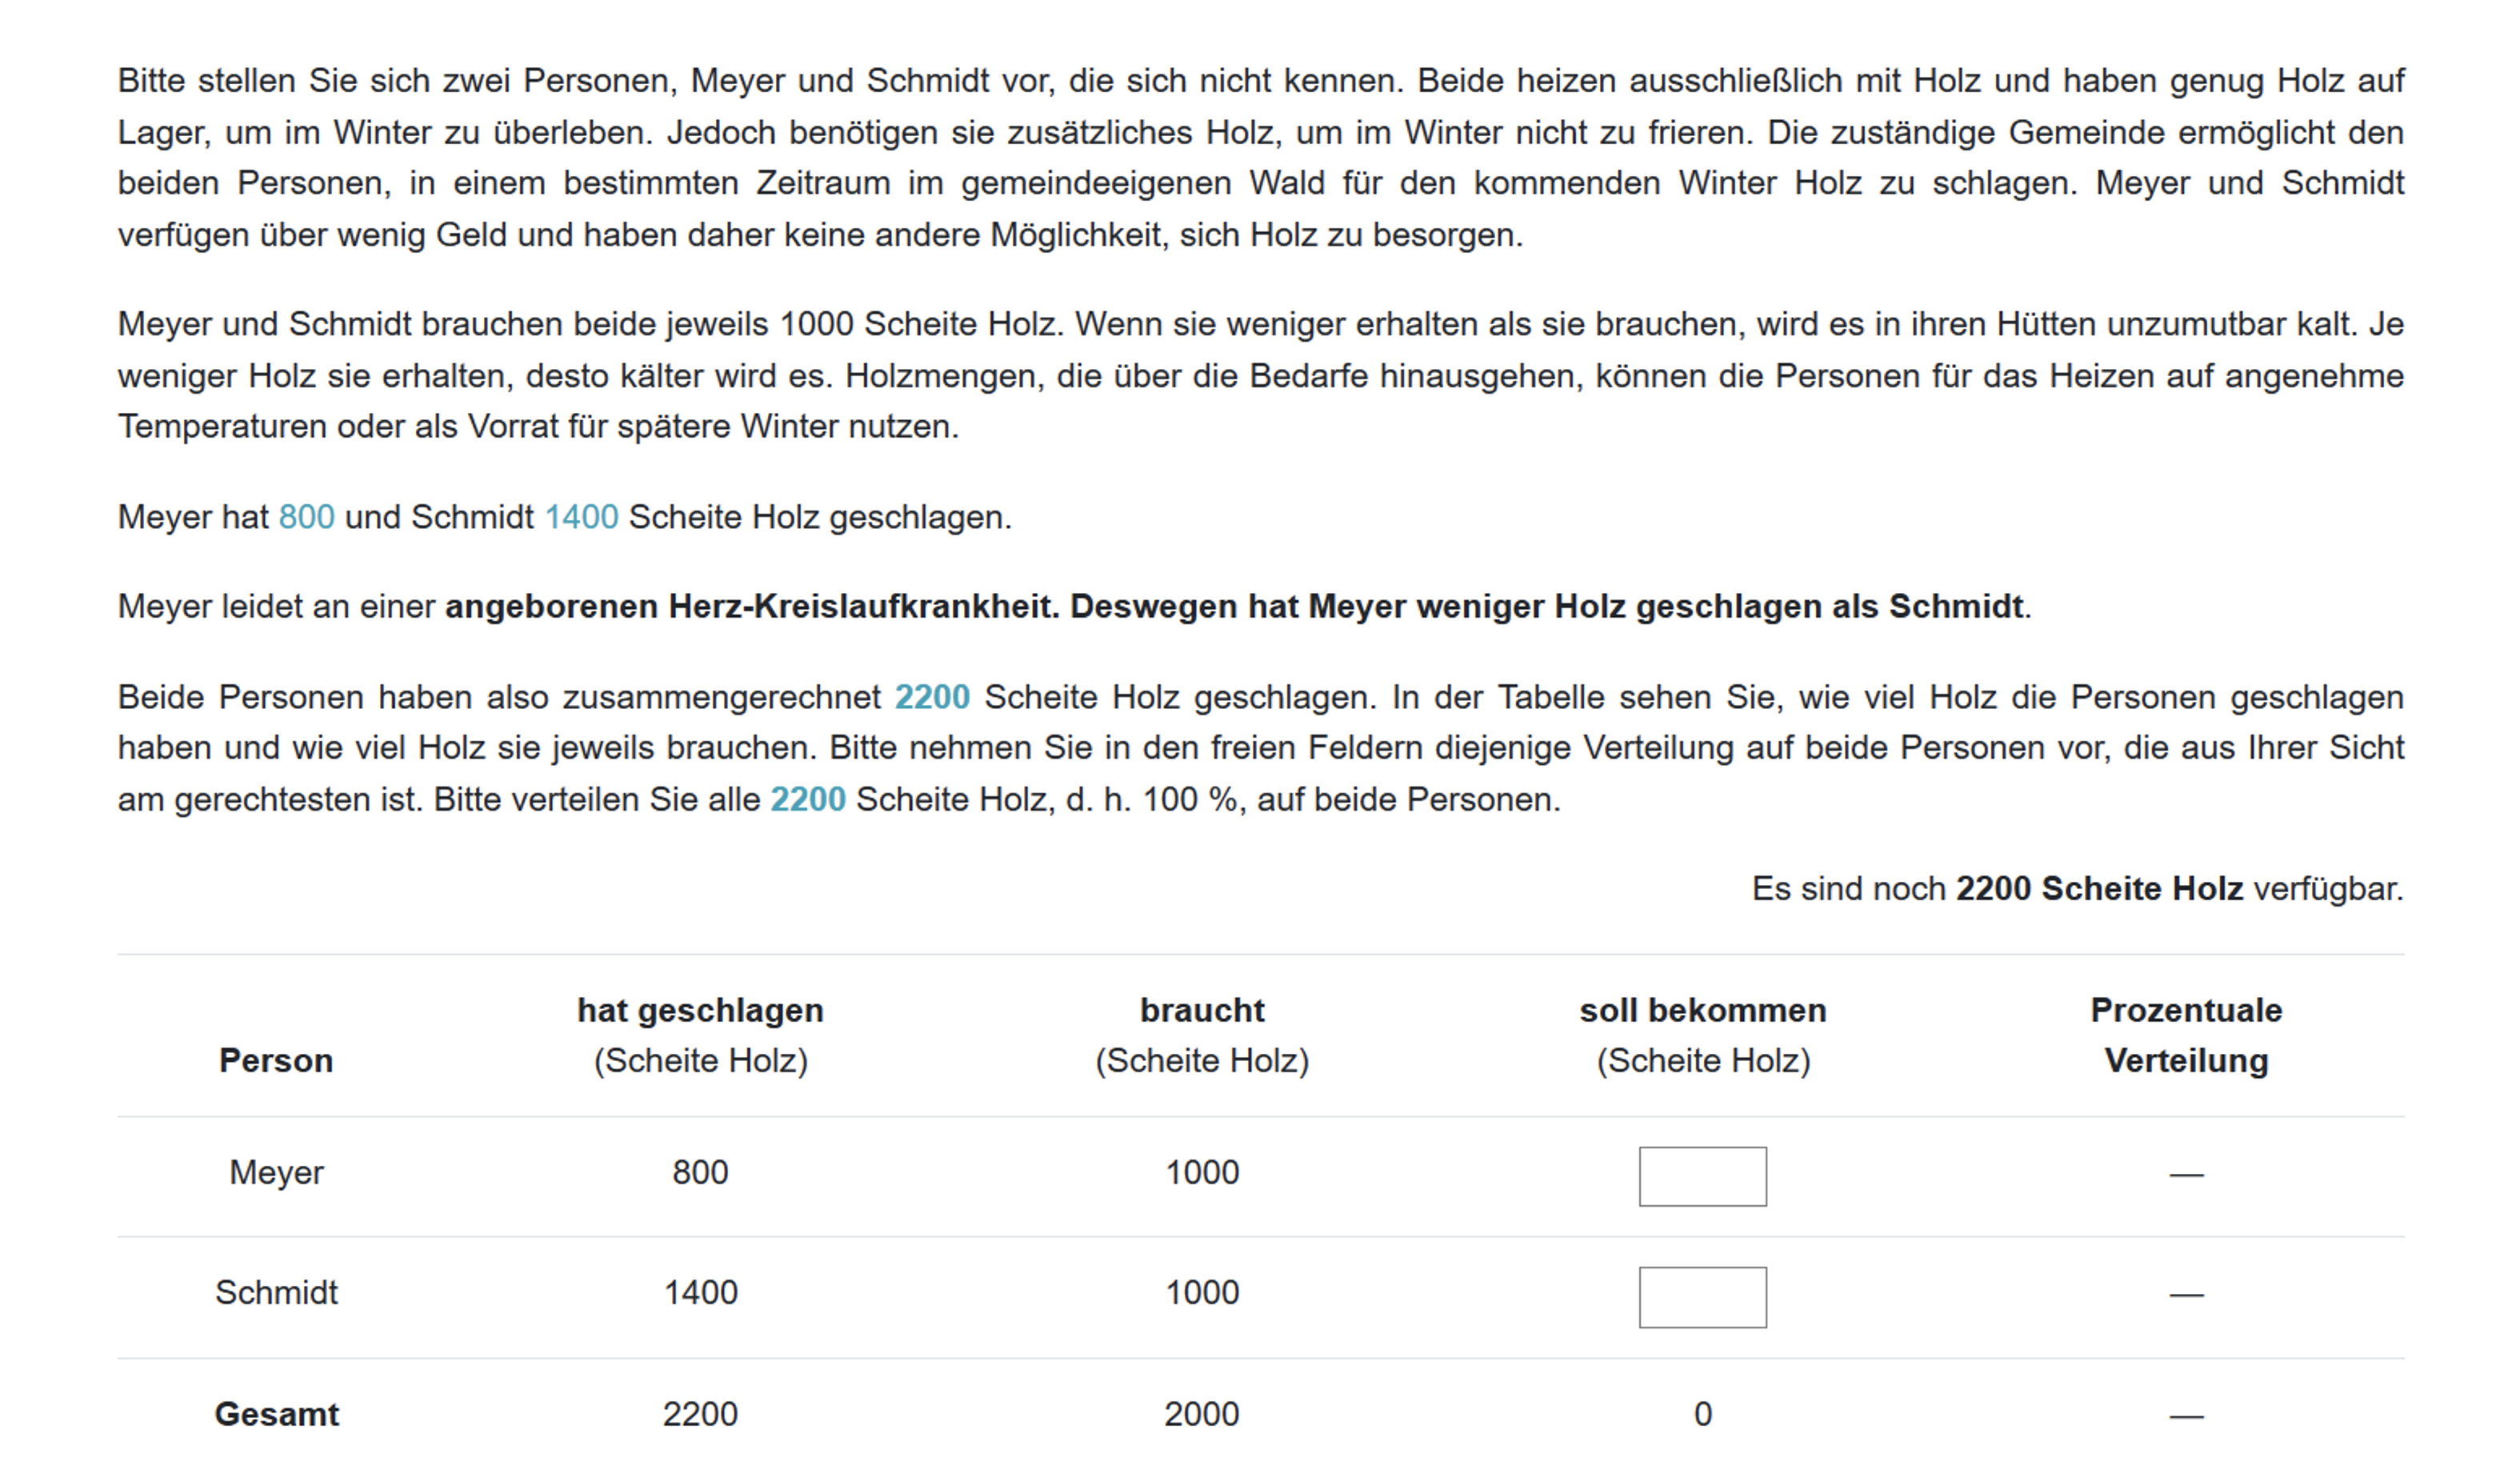
\includegraphics[width=0.5\linewidth]{figures/slides_otree_1.png}}\\
   \textcolor{gray}{Abfragebildschirm\\(Nichtverantwortlichkeitsgruppe, Produktivitätsszenario)}
\end{center}
\end{frame}


%%%%%%%%%%%%
% FOLIE 30 %
%%%%%%%%%%%%
\begin{frame}{\vspace*{10mm}5\hspace*{1em}Bedarf und Verantwortung}
\textbf{Ergebnisse (1/3)}\\
\medskip
\begin{center}
   \frame{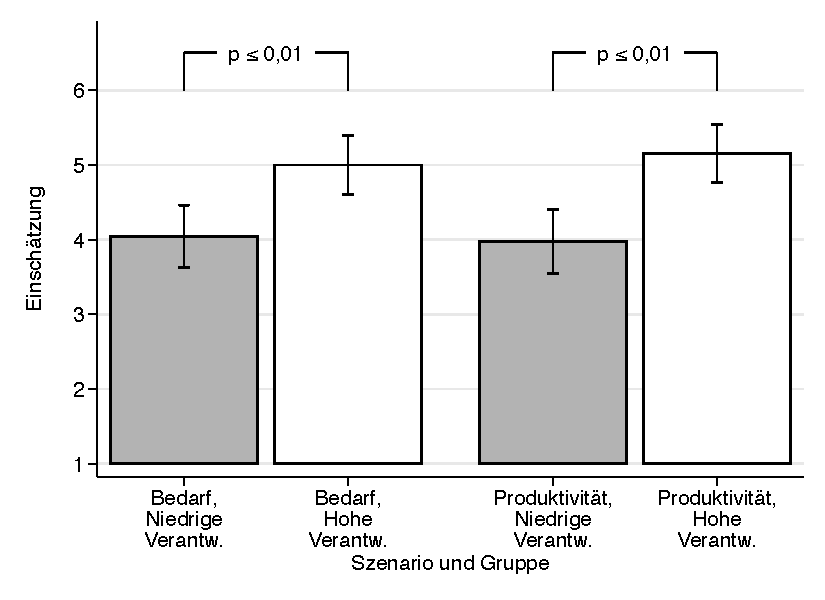
\includegraphics[width=0.5\linewidth]{figures/figure_6.pdf}}\\
   \textcolor{gray}{Einschätzung Verantwortlichkeit}
\end{center}
\end{frame}


%%%%%%%%%%%%
% FOLIE 31 %
%%%%%%%%%%%%
\begin{frame}{\vspace*{10mm}5\hspace*{1em}Bedarf und Verantwortung}
\textbf{Ergebnisse (2/3)}\\
\medskip
\begin{center}
   \frame{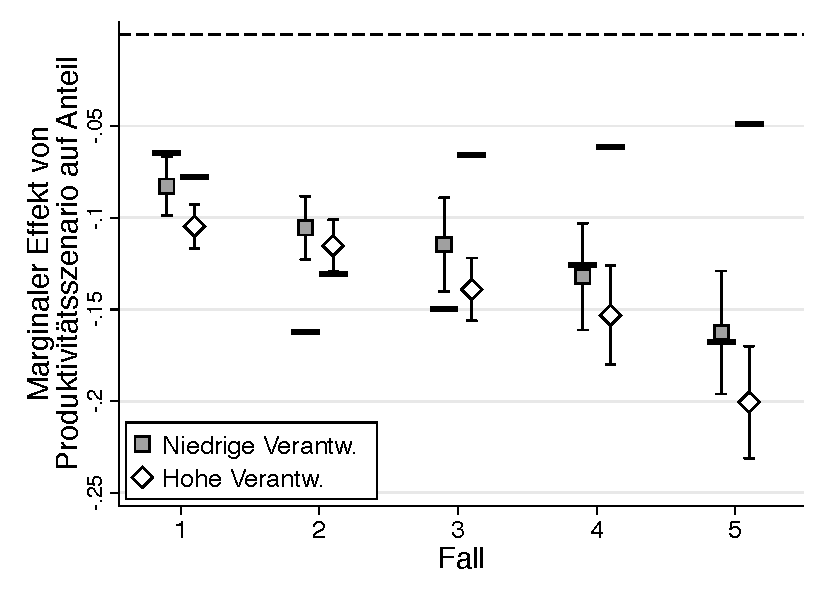
\includegraphics[width=0.5\linewidth]{figures/figure_7_a.pdf}}\\
   \textcolor{gray}{Anteil Person A}
\end{center}
\note{
   \begin{itemize}
      \item $2.000$ Verteilungsentscheidungen ($10\times200$)
      \item Durchgehende Linie: Bedarfsanteil Person A
      \item Gestrichelte Linie: Produktivitätsanteil Person A
   \end{itemize}
}
\end{frame}


%%%%%%%%%%%%
% FOLIE 32 %
%%%%%%%%%%%%
\begin{frame}{\vspace*{10mm}5\hspace*{1em}Bedarf und Verantwortung}
\textbf{Ergebnisse (3/3)}\\
\medskip
\begin{itemize}
   \item Unparteiische Entscheider*innen berücksichtigen Bedarf, Leistung und Verantwortung
   \item Auch bei zu geringer Leistung wird Bedarf teilweise kompensiert
   \item Kompensationsbereitschaft sinkt, wenn zu geringe Leistung oder zu hoher Bedarf selbst verschuldet ist
\end{itemize}
\end{frame}


%%%%%%%%%%%%
% FOLIE 33 %
%%%%%%%%%%%%
\begin{frame}{\vspace*{10mm}5\hspace*{1em}Bedarf und Verantwortung}
\begin{multicols}{2}
   \textbf{Replikation}\\
   \medskip
   \begin{itemize}
      \item Respondi, Online-Panel, November 2020
      \item $n=400$ (stratifiziert wie oben)
      \item Unparteiische Entscheider*innen
      \item Verantwortlichkeits- und Nichtverantwortlichkeitsgruppe (\textit{within subject})
      \item Über- und Unterversorgungsszenario (\textit{within subject})
      \item $10$ Verteilungsaufgaben, eingebettet in hypothetischen Kontext
   \end{itemize}
   \vfill
   \begin{center}
      \frame{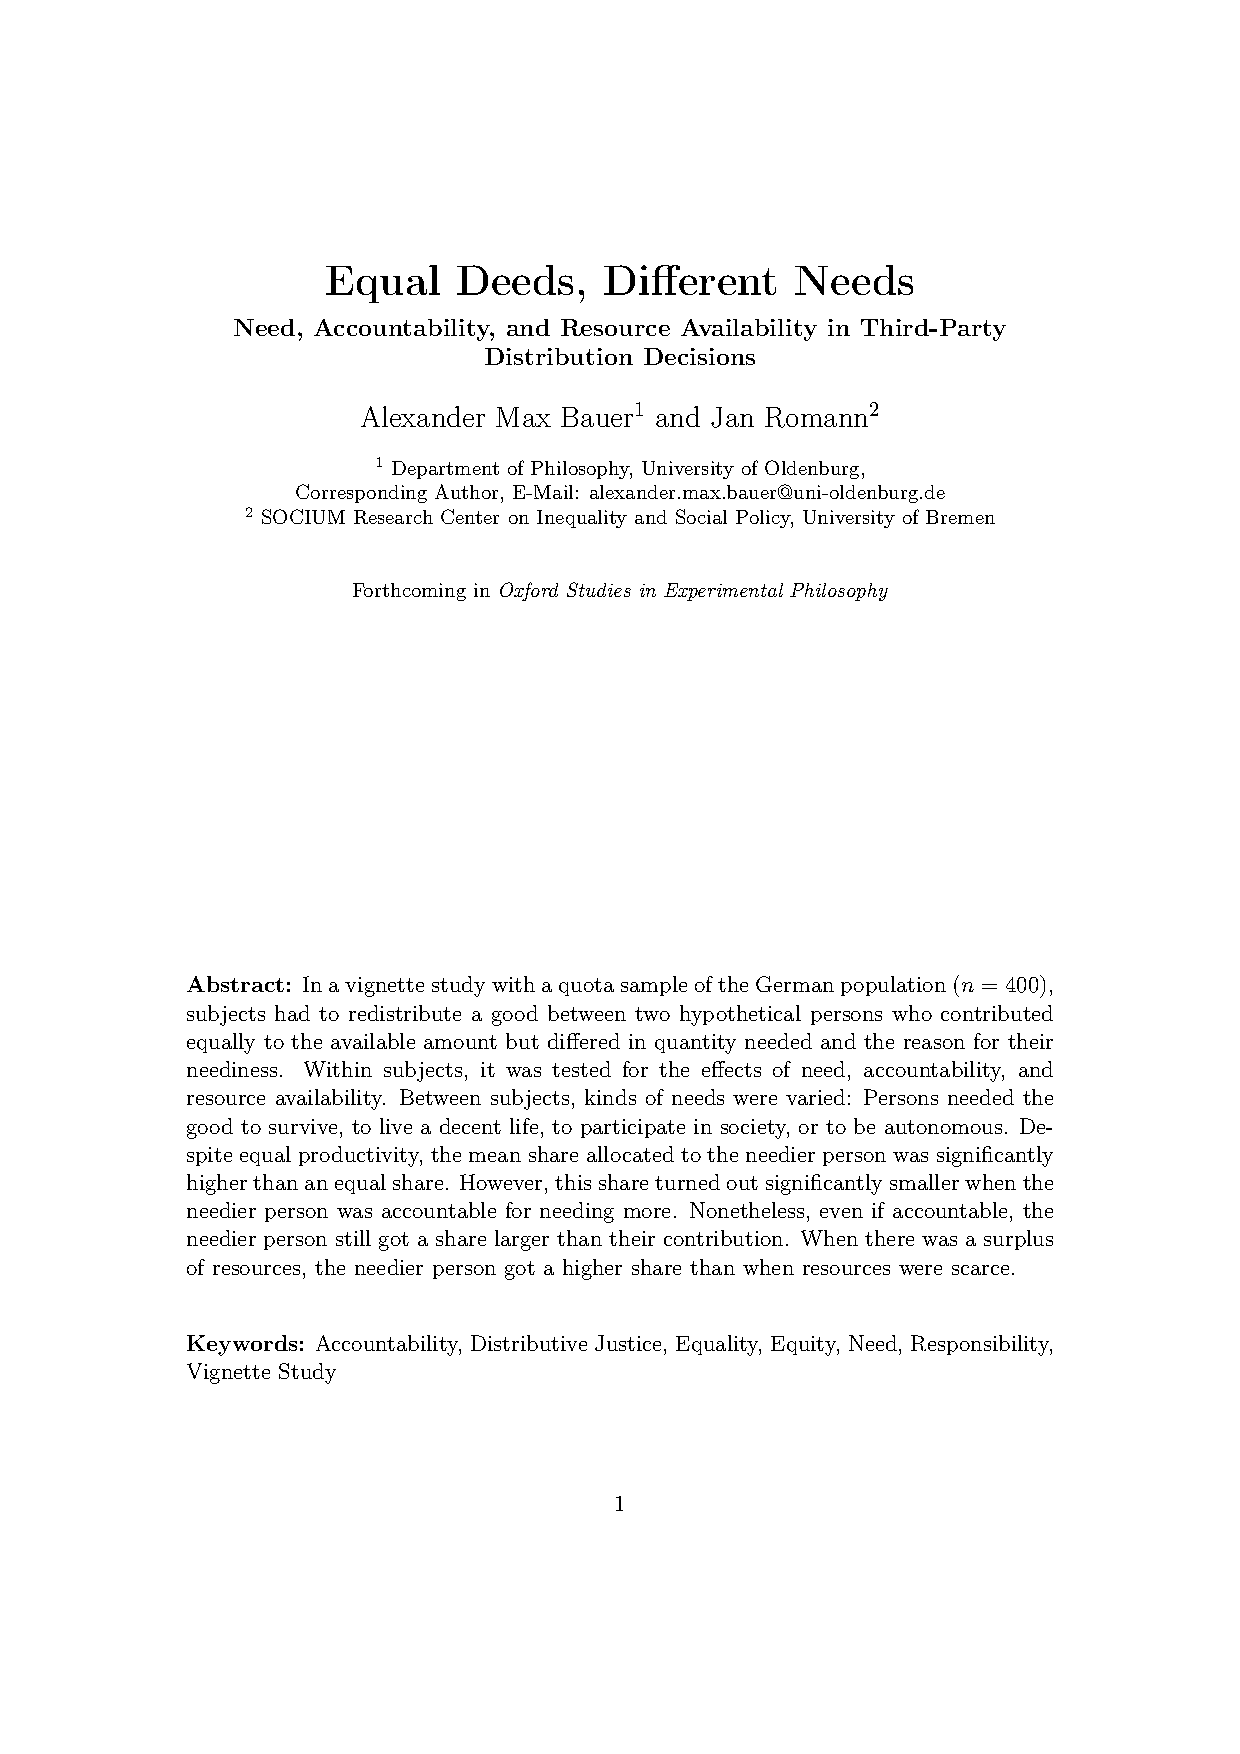
\includegraphics[width=0.6\linewidth]{figures/slides_bauer_romann_nd.pdf}}\\
      \textcolor{gray}{Bauer und Romann i.\,V.}
   \end{center}
\end{multicols}
\end{frame}


%%%%%%%%%%%%
% FOLIE 34 %
%%%%%%%%%%%%
\begin{frame}
\begin{overlayarea}{\textwidth}{0.81\paperheight}{
   \vspace*{11mm}
   \usebeamerfont{title}\textcolor{uolblue}
   {6\hspace*{1em}Bedarfsarten}
}
\end{overlayarea}
\end{frame}


%%%%%%%%%%%%
% FOLIE 35 %
%%%%%%%%%%%%
\begin{frame}{\vspace*{10mm}6\hspace*{1em}Bedarfsarten}
\begin{multicols}{2}
   \textbf{Hintergrund}\\
   \medskip
   \begin{itemize}
      \item Philosophische Literatur unterscheidet zwischen verschiedenen Bedarfsarten
      \item Welche Rolle spielen unterschiedliche Bedarfsarten bei unparteiischen Verteilungsentscheidungen?
   \end{itemize}
   \vfill
   \begin{center}
      \frame{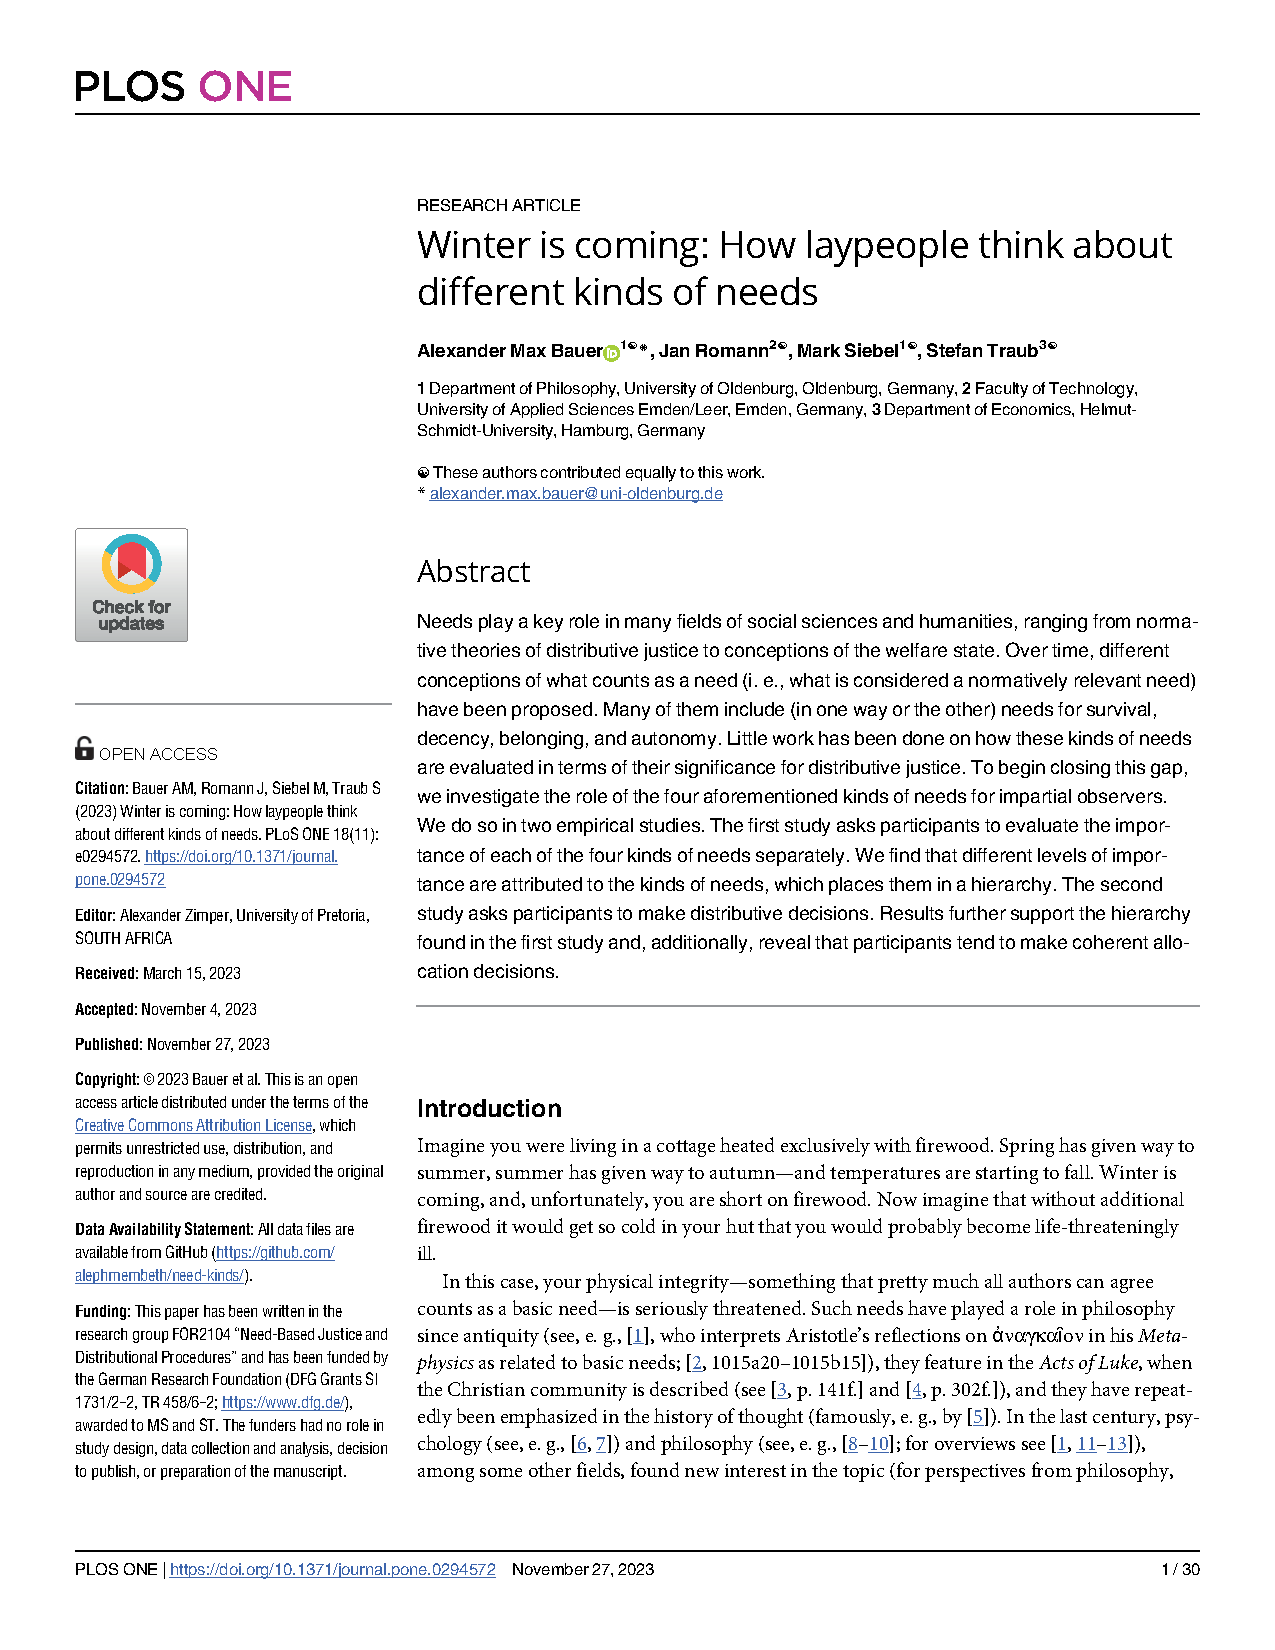
\includegraphics[width=0.6\linewidth]{figures/slides_bauer_et_al_2023b.pdf}}\\
      \textcolor{gray}{Bauer et al. 2023b}
   \end{center}
\end{multicols}
\end{frame}


%%%%%%%%%%%%
% FOLIE 36 %
%%%%%%%%%%%%
\begin{frame}
\begin{overlayarea}{\textwidth}{0.81\paperheight}{
   \vspace*{11mm}
   \usebeamerfont{title}\textcolor{uolblue}
   {6.1\hspace*{1em}Studie 1}
}
\end{overlayarea}
\end{frame}


%%%%%%%%%%%%
% FOLIE 37 %
%%%%%%%%%%%%
\begin{frame}{\vspace*{10mm}6.1\hspace*{1em}Studie 1}
\textbf{Design und Durchführung}\\
\medskip
\begin{itemize}
   \item Respondi, Online-Panel, Februar 2021
   \item $n=100$ (stratifiziert wie oben)
   \item Unparteiische Beobachter*innen
   \item $4$ Bedarfsarten (\textit{within subjects})
   \item $4$ Einschätzungsaufgaben, eingebettet in hypothetischen Kontext
\end{itemize}
\end{frame}


%%%%%%%%%%%%
% FOLIE 38 %
%%%%%%%%%%%%
\begin{frame}{\vspace*{10mm}6.1\hspace*{1em}Studie 1}
\textbf{Vignette (1/5)}\\
\medskip
\enquote{Bitte stellen Sie sich vier Personen mit den Namen $A$, $B$, $C$ und $D$ vor. Jede dieser Personen benötigt Feuerholz. Sie benötigen das Feuerholz aus unterschiedlichen Gründen. Auf dieser Seite stellen wir Ihnen vor, wofür $A$, $B$, $C$ und $D$ das Feuerholz jeweils benötigen. Auf den kommenden Seiten werden wir Sie fragen, für wie wichtig Sie es halten, dass der Bedarf dieser Personen erfüllt wird.}
\end{frame}


%%%%%%%%%%%%
% FOLIE 39 %
%%%%%%%%%%%%
\begin{frame}{\vspace*{10mm}6.1\hspace*{1em}Studie 1}
\begin{multicols}{2}
   \textbf{Vignette (2/5)}\\
   \medskip
   \enquote{$A$ benötigt das Holz, um sicherzustellen, dass er den kommenden Winter überlebt. Wenn $A$ weniger erhält als er braucht, wird es in seiner Hütte so kalt, dass er mit hoher Wahrscheinlichkeit lebensbedrohlich erkrankt. Je weniger Holz er erhält, desto höher ist die Wahrscheinlichkeit, dass er lebensbedrohlich erkrankt.}
   \vfill
   \begin{center}
      \frame{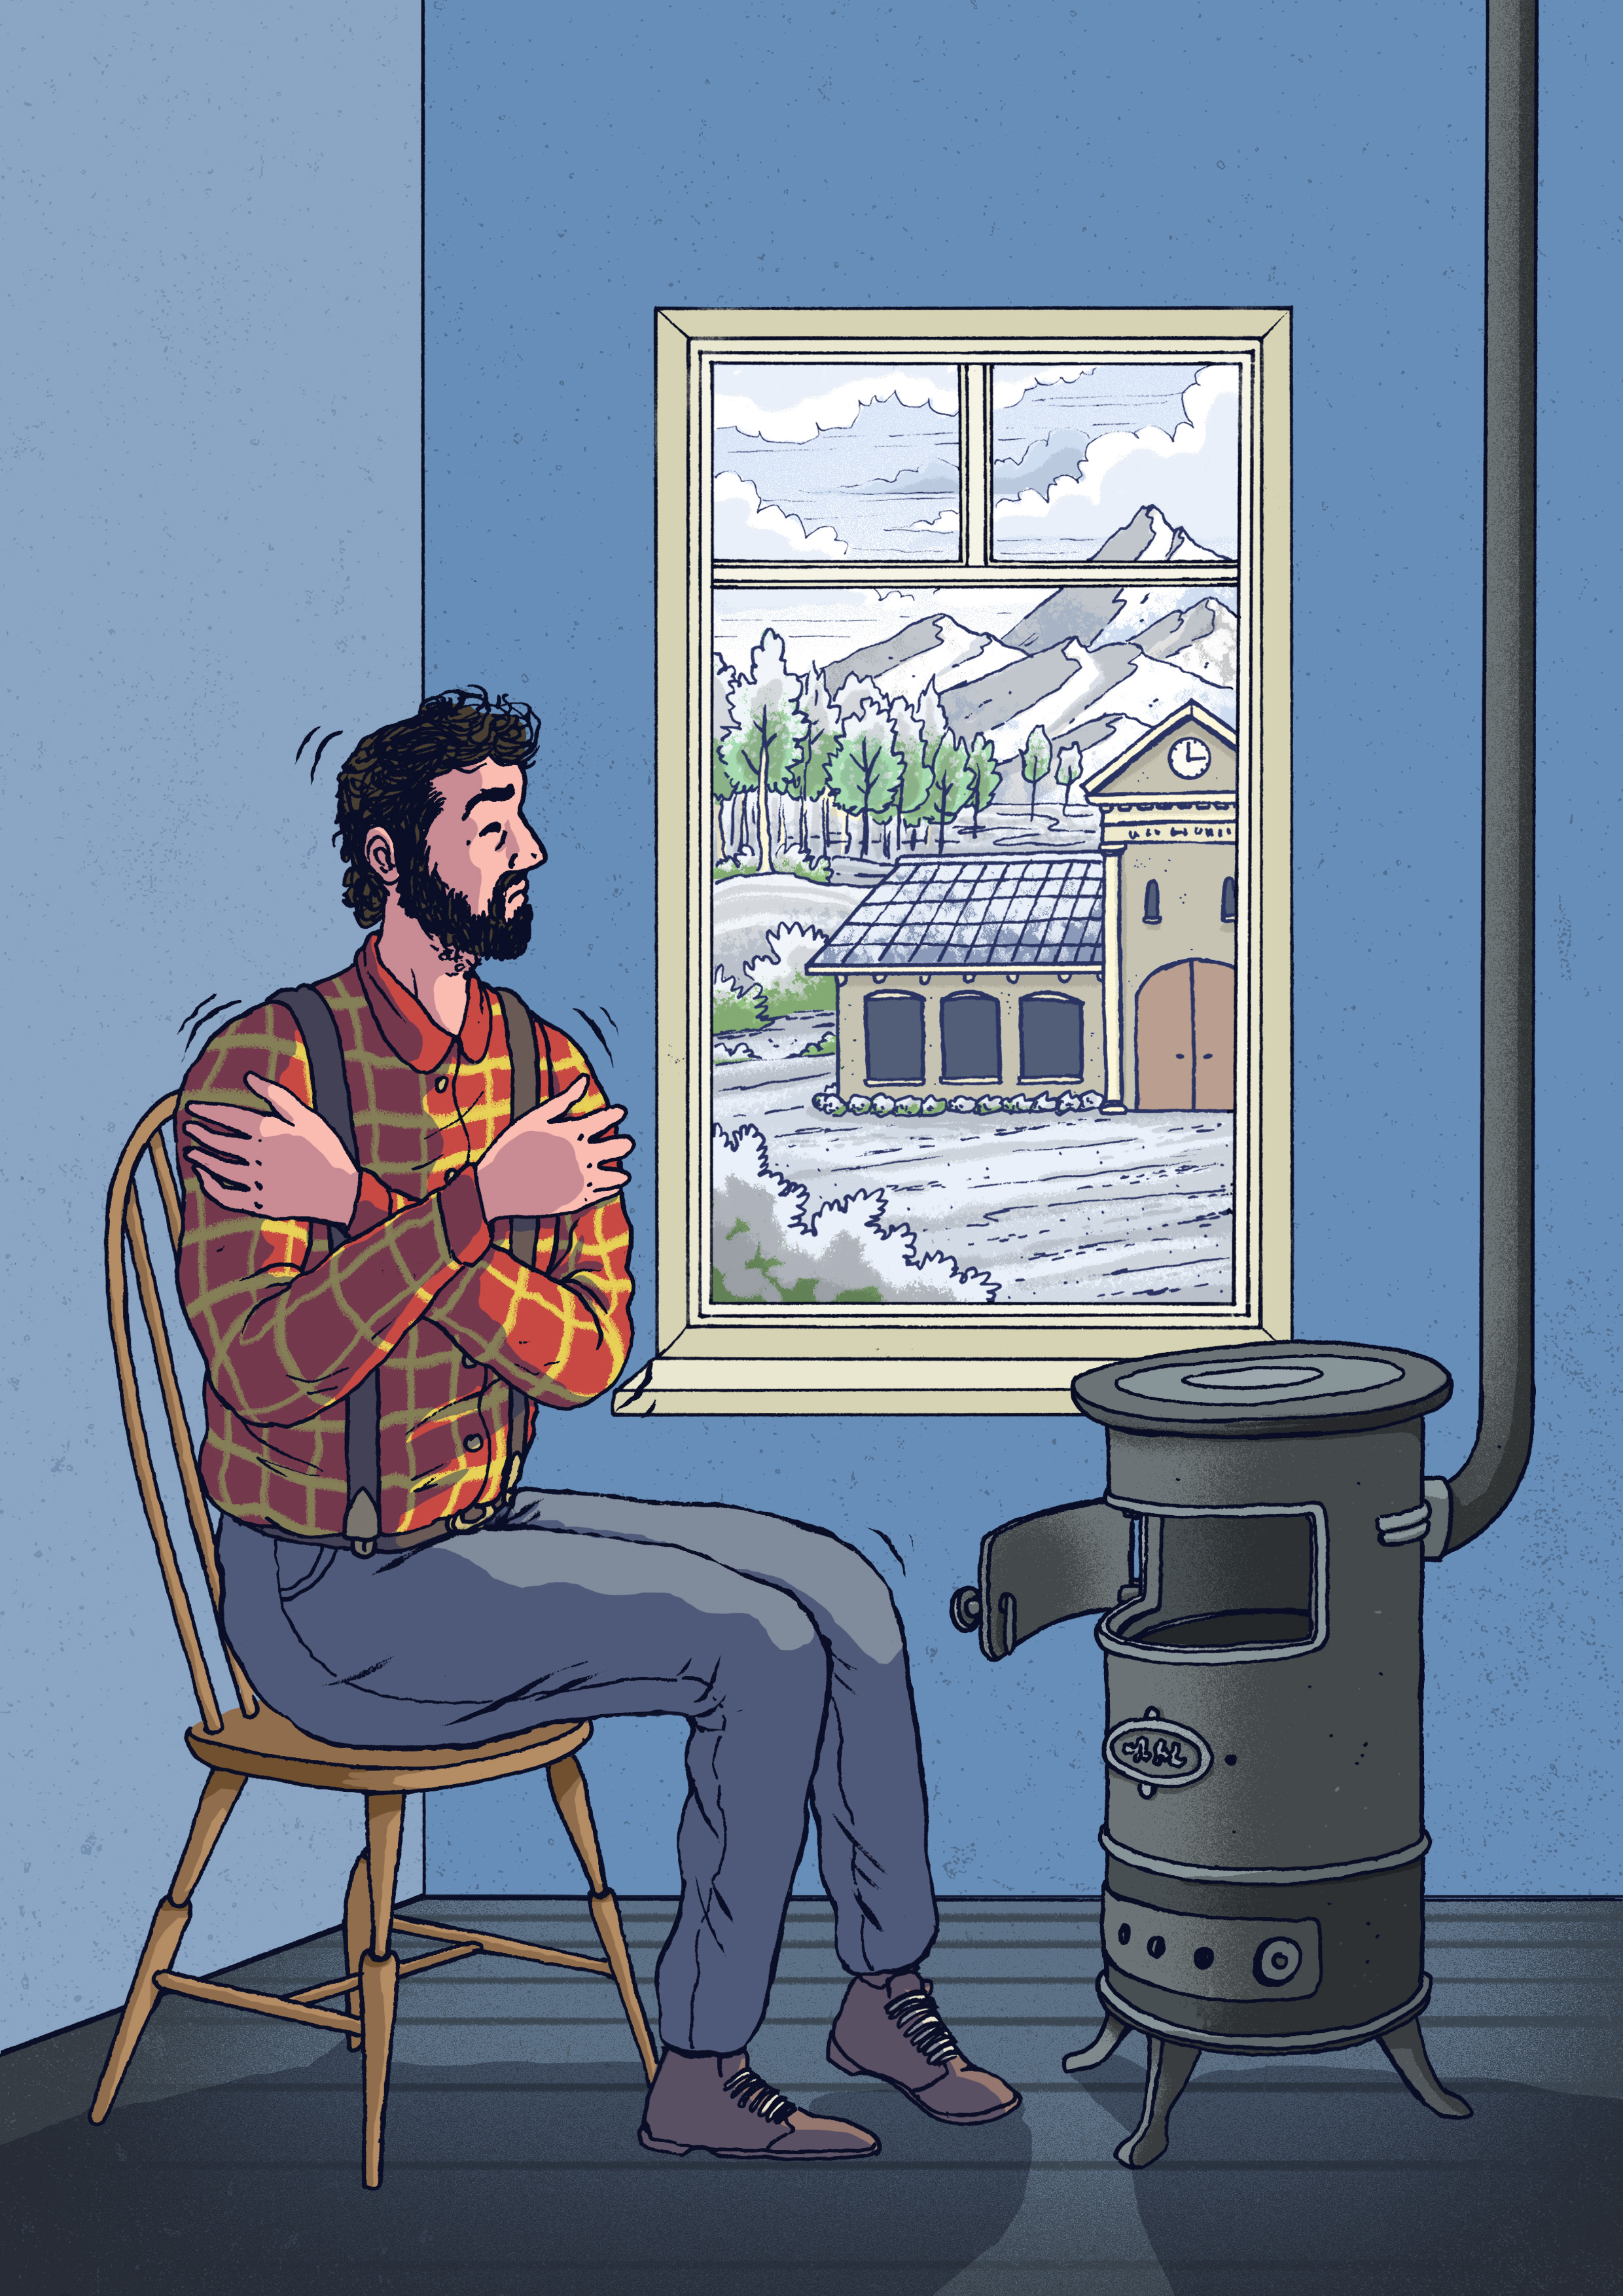
\includegraphics[width=0.6\linewidth]{figures/figure_11.jpg}}\\
      \textcolor{gray}{Illustration \textit{Überleben}}
   \end{center}
\end{multicols}
\end{frame}


%%%%%%%%%%%%
% FOLIE 40 %
%%%%%%%%%%%%
\begin{frame}{\vspace*{10mm}6.1\hspace*{1em}Studie 1}
\begin{multicols}{2}
   \textbf{Vignette (3/5)}\\
   \medskip
   \enquote{$B$ benötigt das Holz, um im kommenden Winter nicht zu frieren. Die Mitglieder der Gemeinde, zu der $B$ gehört, sind sich darin einig, dass man nicht in Würde leben kann, wenn man frieren muss. Wenn $B$ weniger erhält als er braucht, wird es in seiner Hütte unannehmbar kalt. Je weniger Holz er erhält, desto häufiger wird er frieren.}
   \vfill
   \begin{center}
      \frame{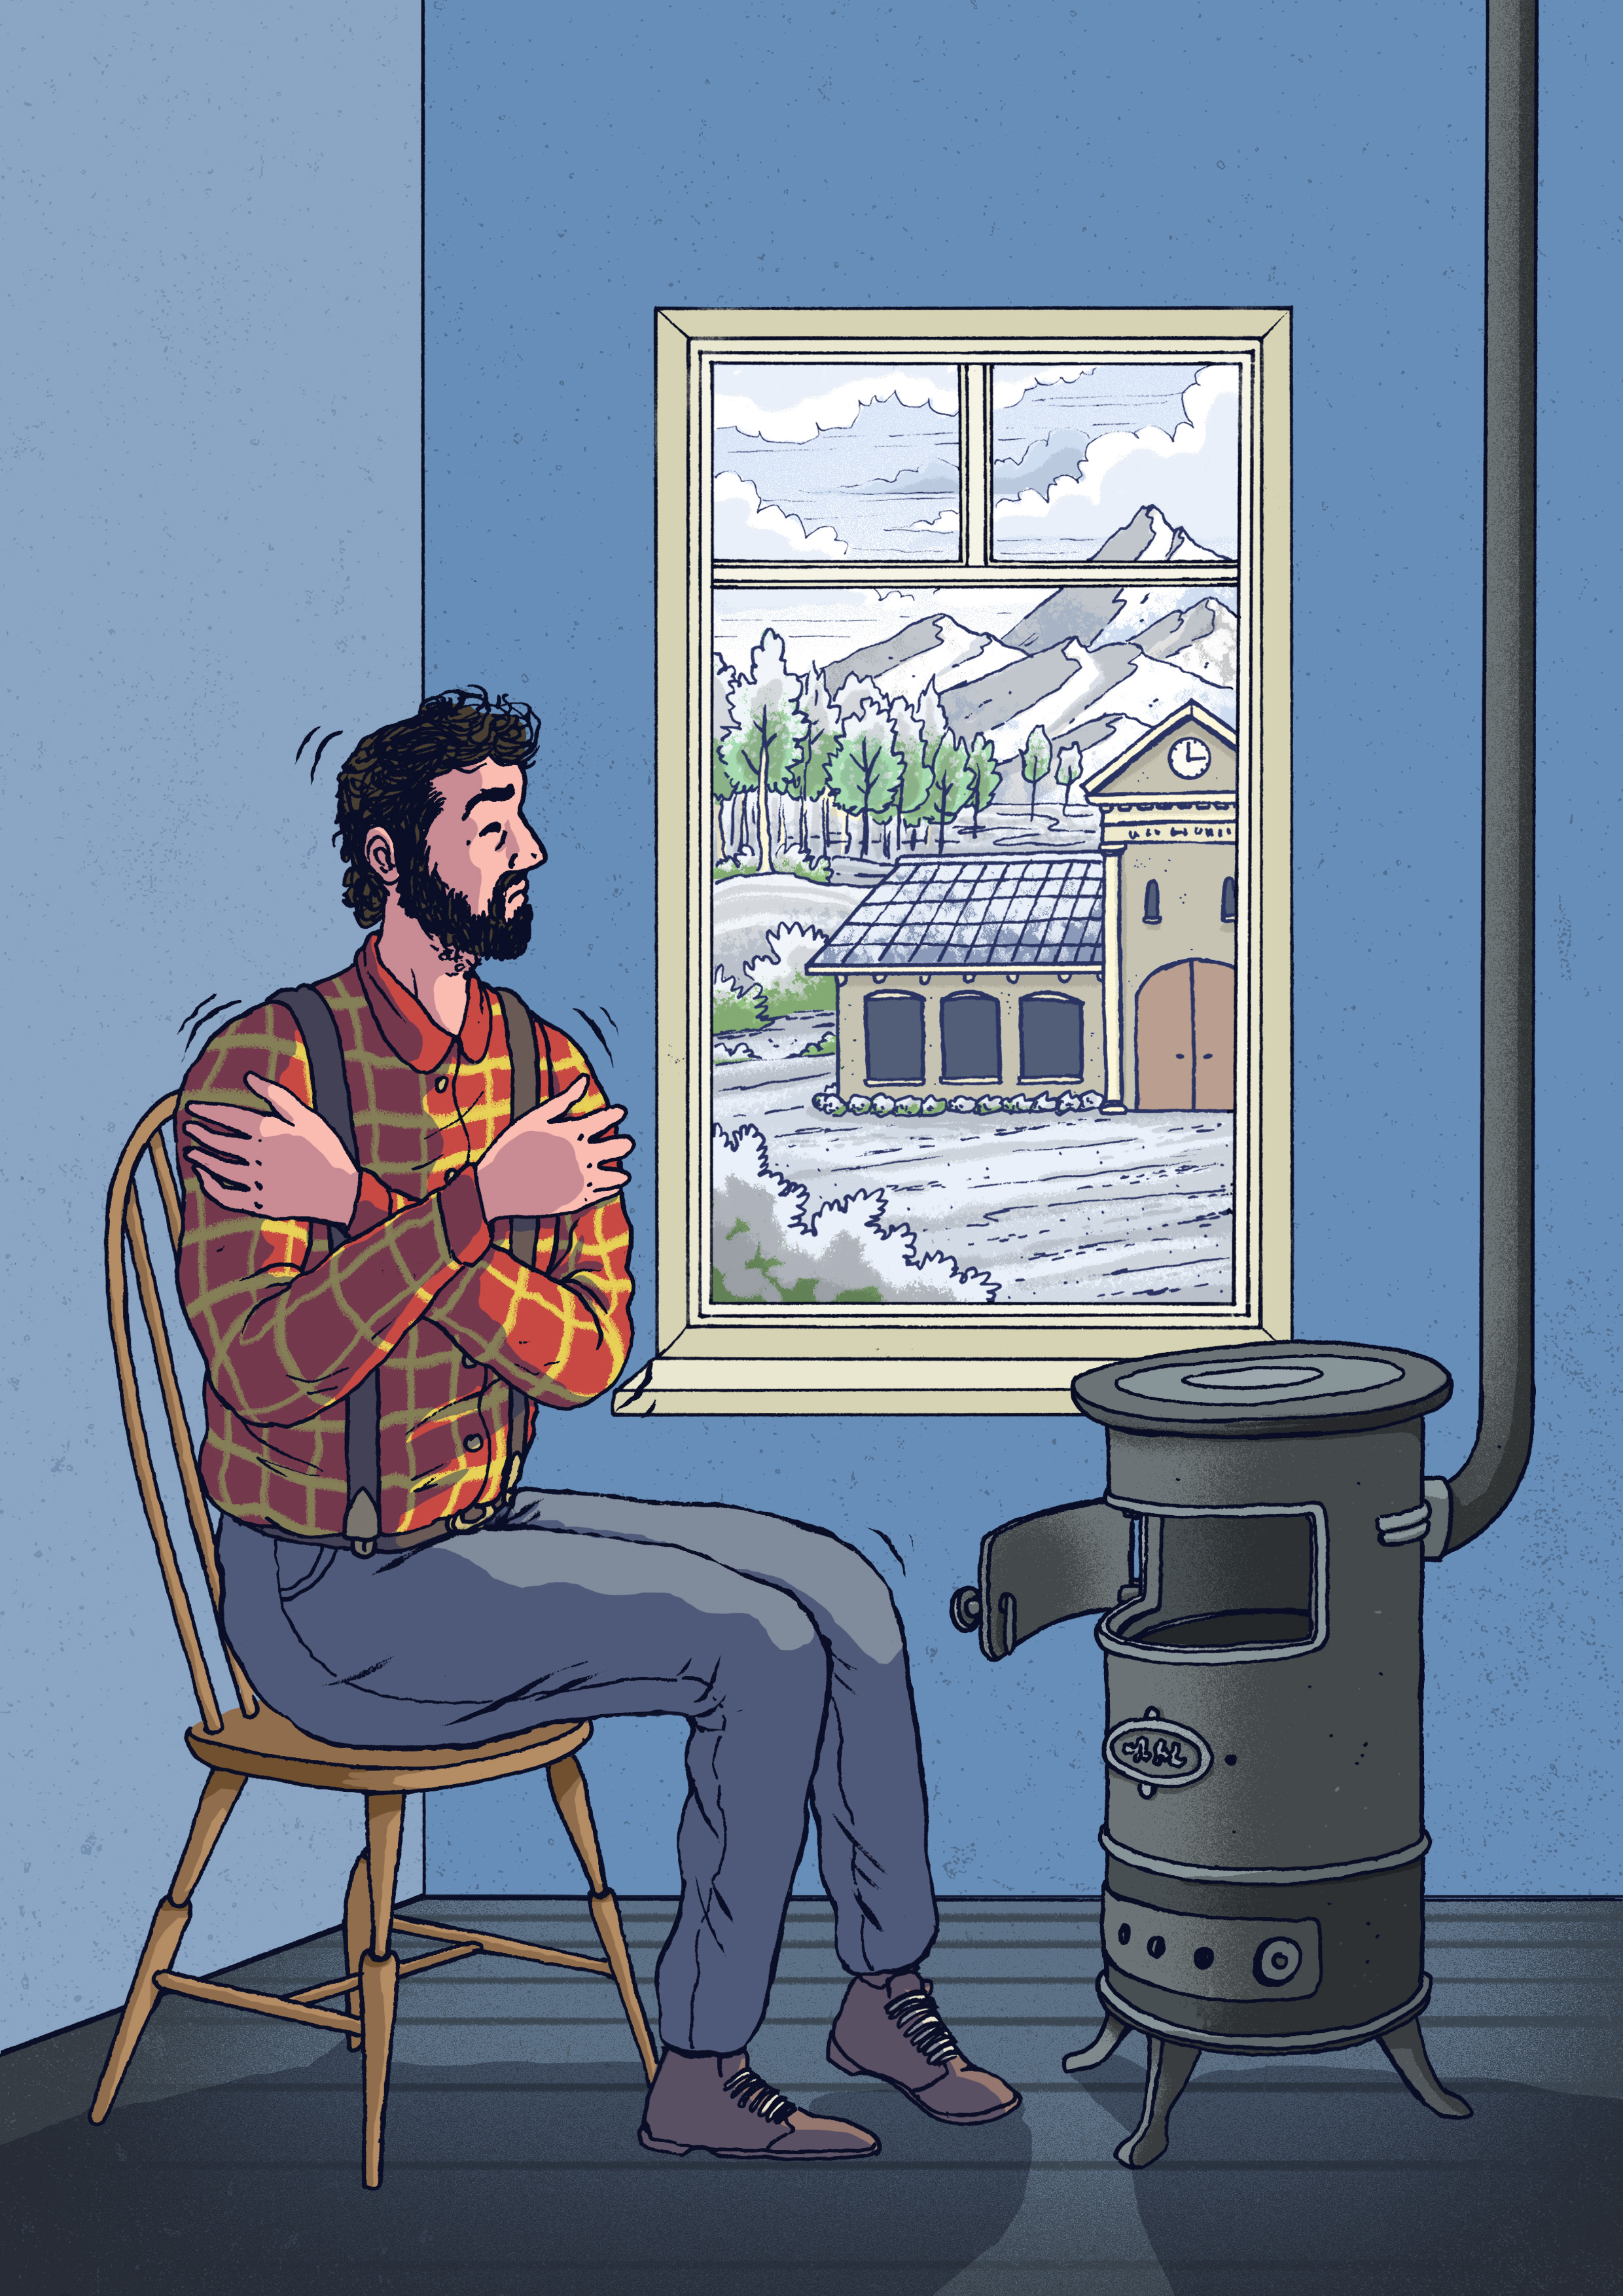
\includegraphics[width=0.6\linewidth]{figures/figure_12.jpg}}\\
      \textcolor{gray}{Illustration \textit{Würde}}
   \end{center}
\end{multicols}
\end{frame}


%%%%%%%%%%%%
% FOLIE 41 %
%%%%%%%%%%%%
\begin{frame}{\vspace*{10mm}6.1\hspace*{1em}Studie 1}
\begin{multicols}{2}
   \textbf{Vignette (4/5)}\\
   \medskip
   \enquote{$C$ benötigt das Holz, um im kommenden Winter regelmäßig am sozialen Leben seiner Gemeinde teilhaben zu können. Es ist Gang und Gäbe, dass man sich im Gemeindehaus trifft und jeder Holz mitbringt, mit dem es beheizt werden kann. Wenn $C$ weniger erhält als er braucht, wird er nicht regelmäßig am sozialen Leben teilhaben können. Je weniger Holz er erhält, desto seltener wird er zu Treffen im Gemeindehaus kommen können.}
   \vfill
   \begin{center}
      \frame{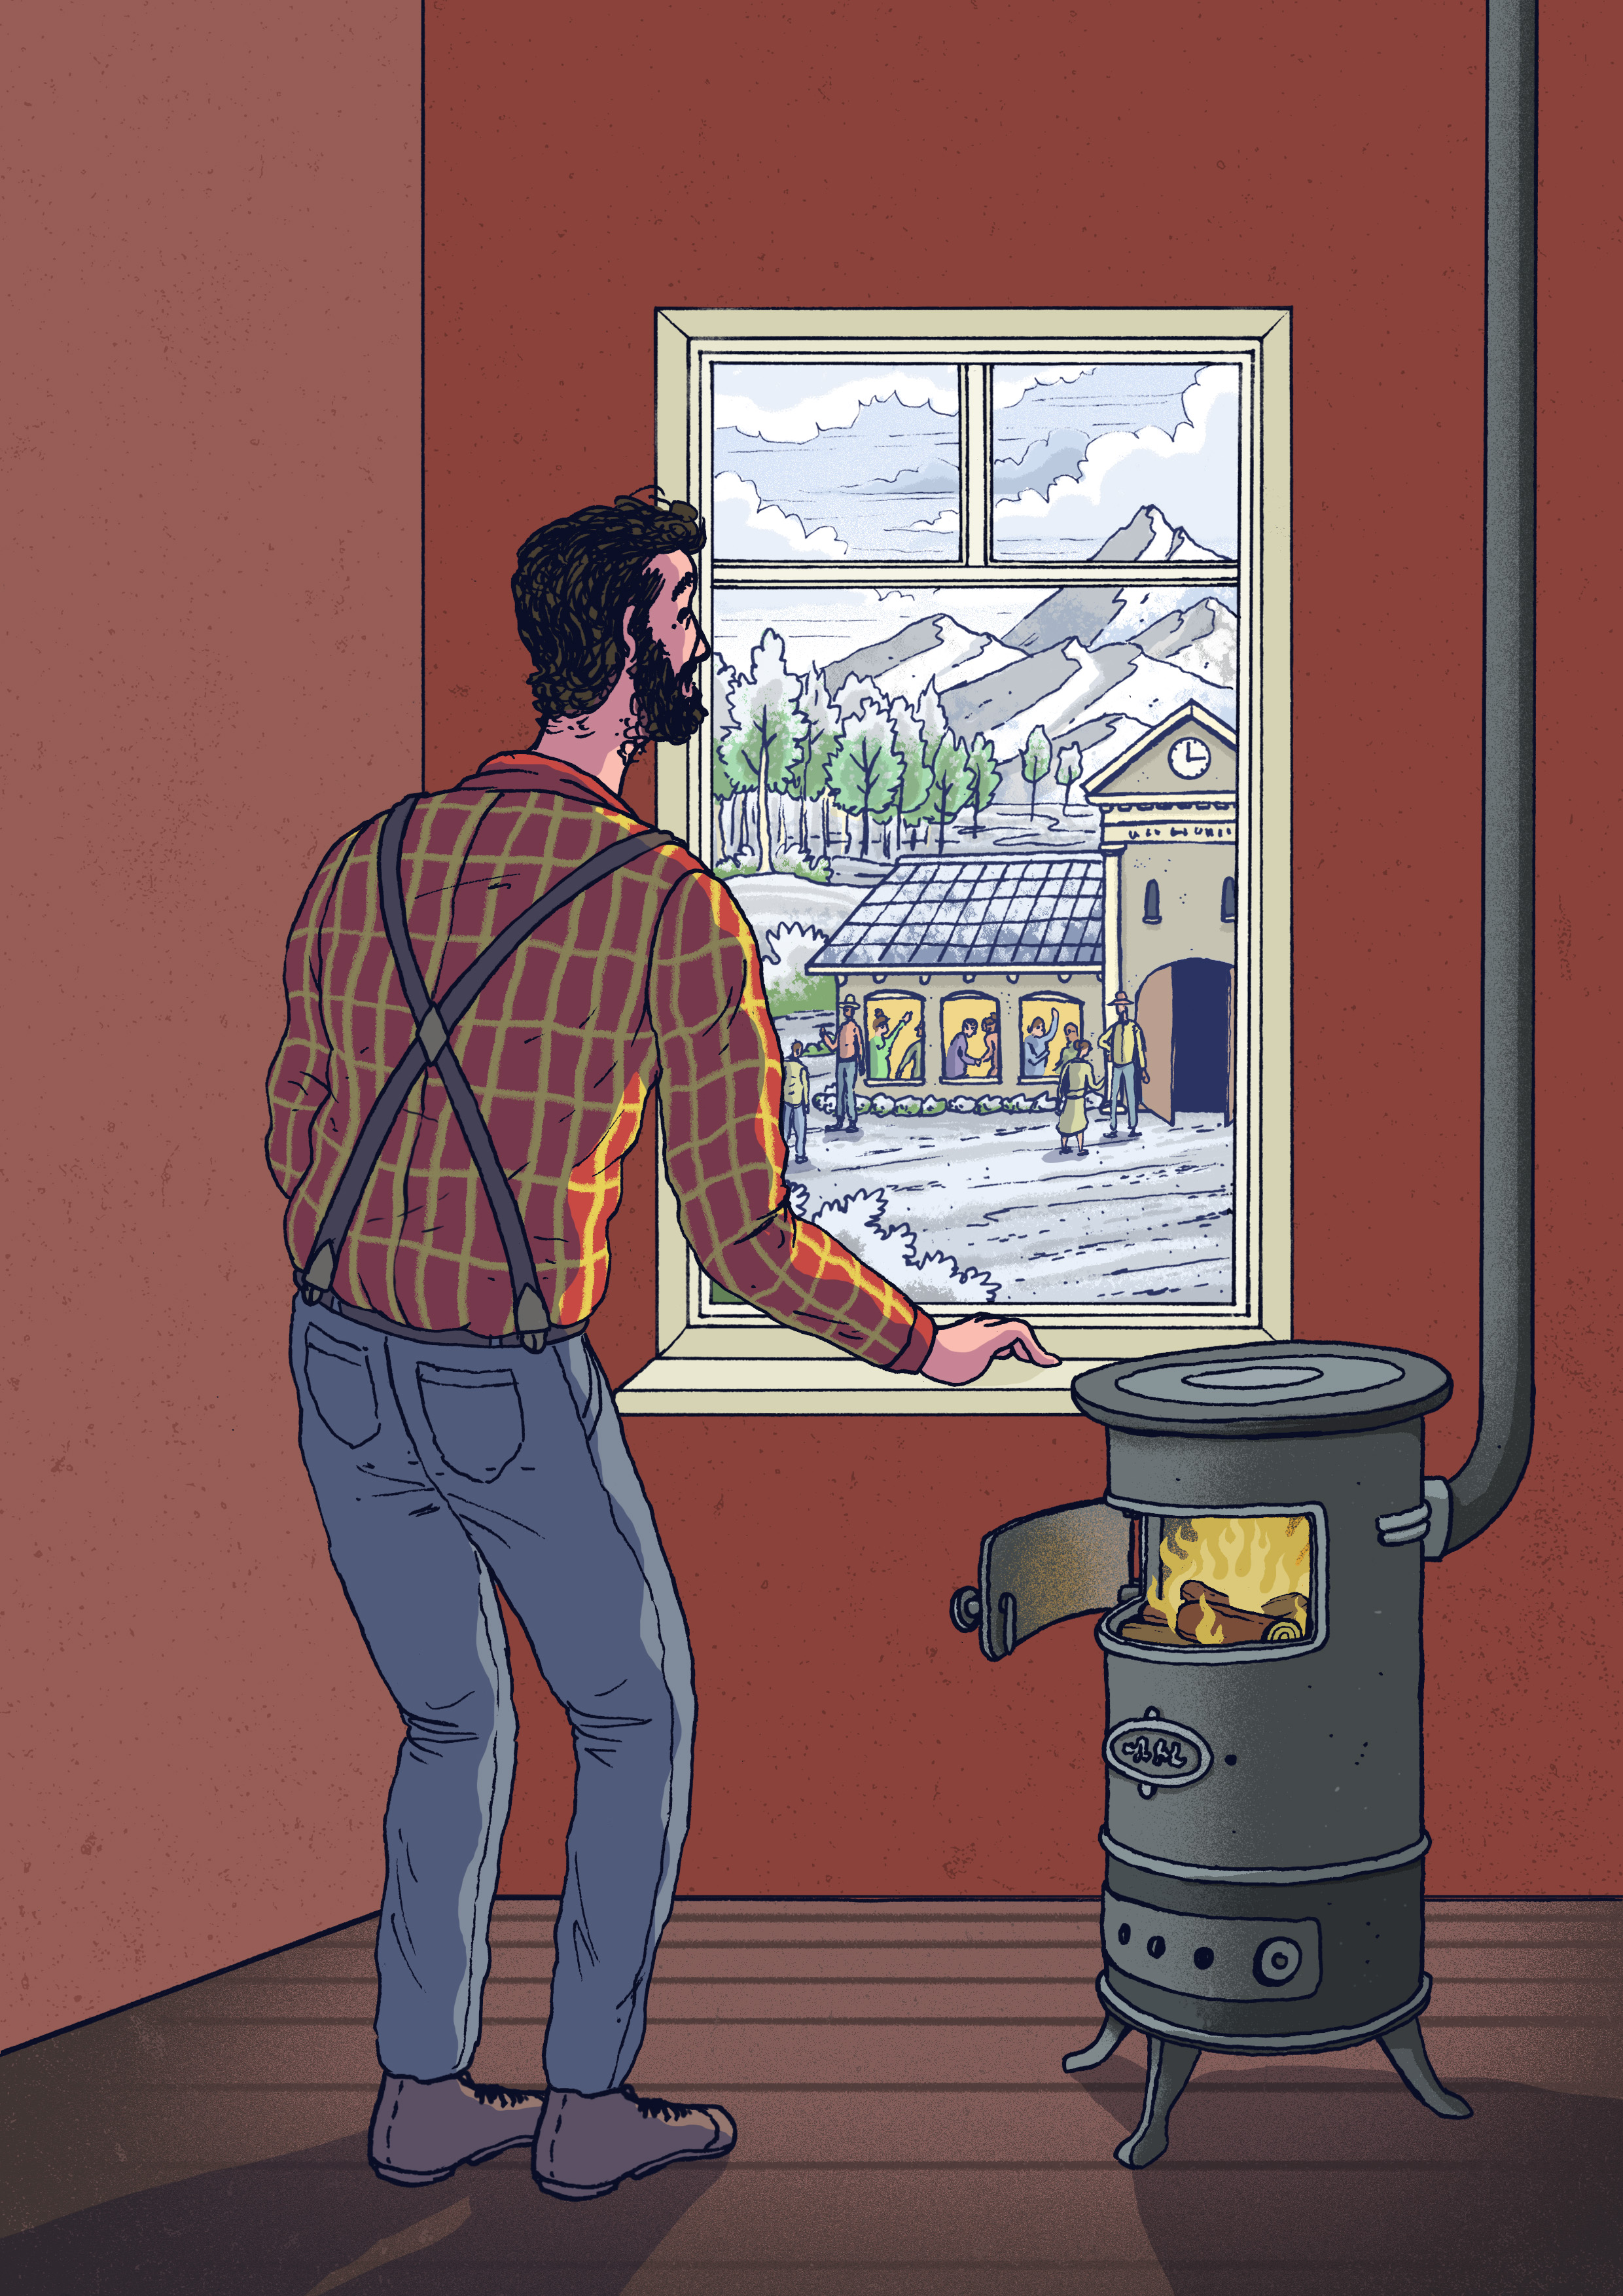
\includegraphics[width=0.6\linewidth]{figures/figure_13.jpg}}\\
      \textcolor{gray}{Illustration \textit{Teilhabe}}
   \end{center}
\end{multicols}
\end{frame}


%%%%%%%%%%%%
% FOLIE 42 %
%%%%%%%%%%%%
\begin{frame}{\vspace*{10mm}6.1\hspace*{1em}Studie 1}
\begin{multicols}{2}
   \textbf{Vignette (5/5)}\\
   \medskip
   \enquote{$D$ benötigt das Holz, um im kommenden Winter regelmäßig sein Atelier nutzen zu können. Dort schafft er in seiner Freizeit Kunst. Wenn $D$ weniger erhält als er braucht, wird er nicht regelmäßig sein Atelier nutzen können. Je weniger Holz er erhält, desto seltener wird er in seinem Atelier Kunst schaffen können.}
   \vfill
   \begin{center}
      \frame{
\includegraphics[width=0.6\linewidth]{figures/figure_14.jpg}}\\
      \textcolor{gray}{Illustration \textit{Autonomie}}
   \end{center}
\end{multicols}
\end{frame}


%%%%%%%%%%%%
% FOLIE 43 %
%%%%%%%%%%%%
\begin{frame}{\vspace*{10mm}6.1\hspace*{1em}Studie 1}
\textbf{Abfrage}\\
\medskip
\begin{center}
   \frame{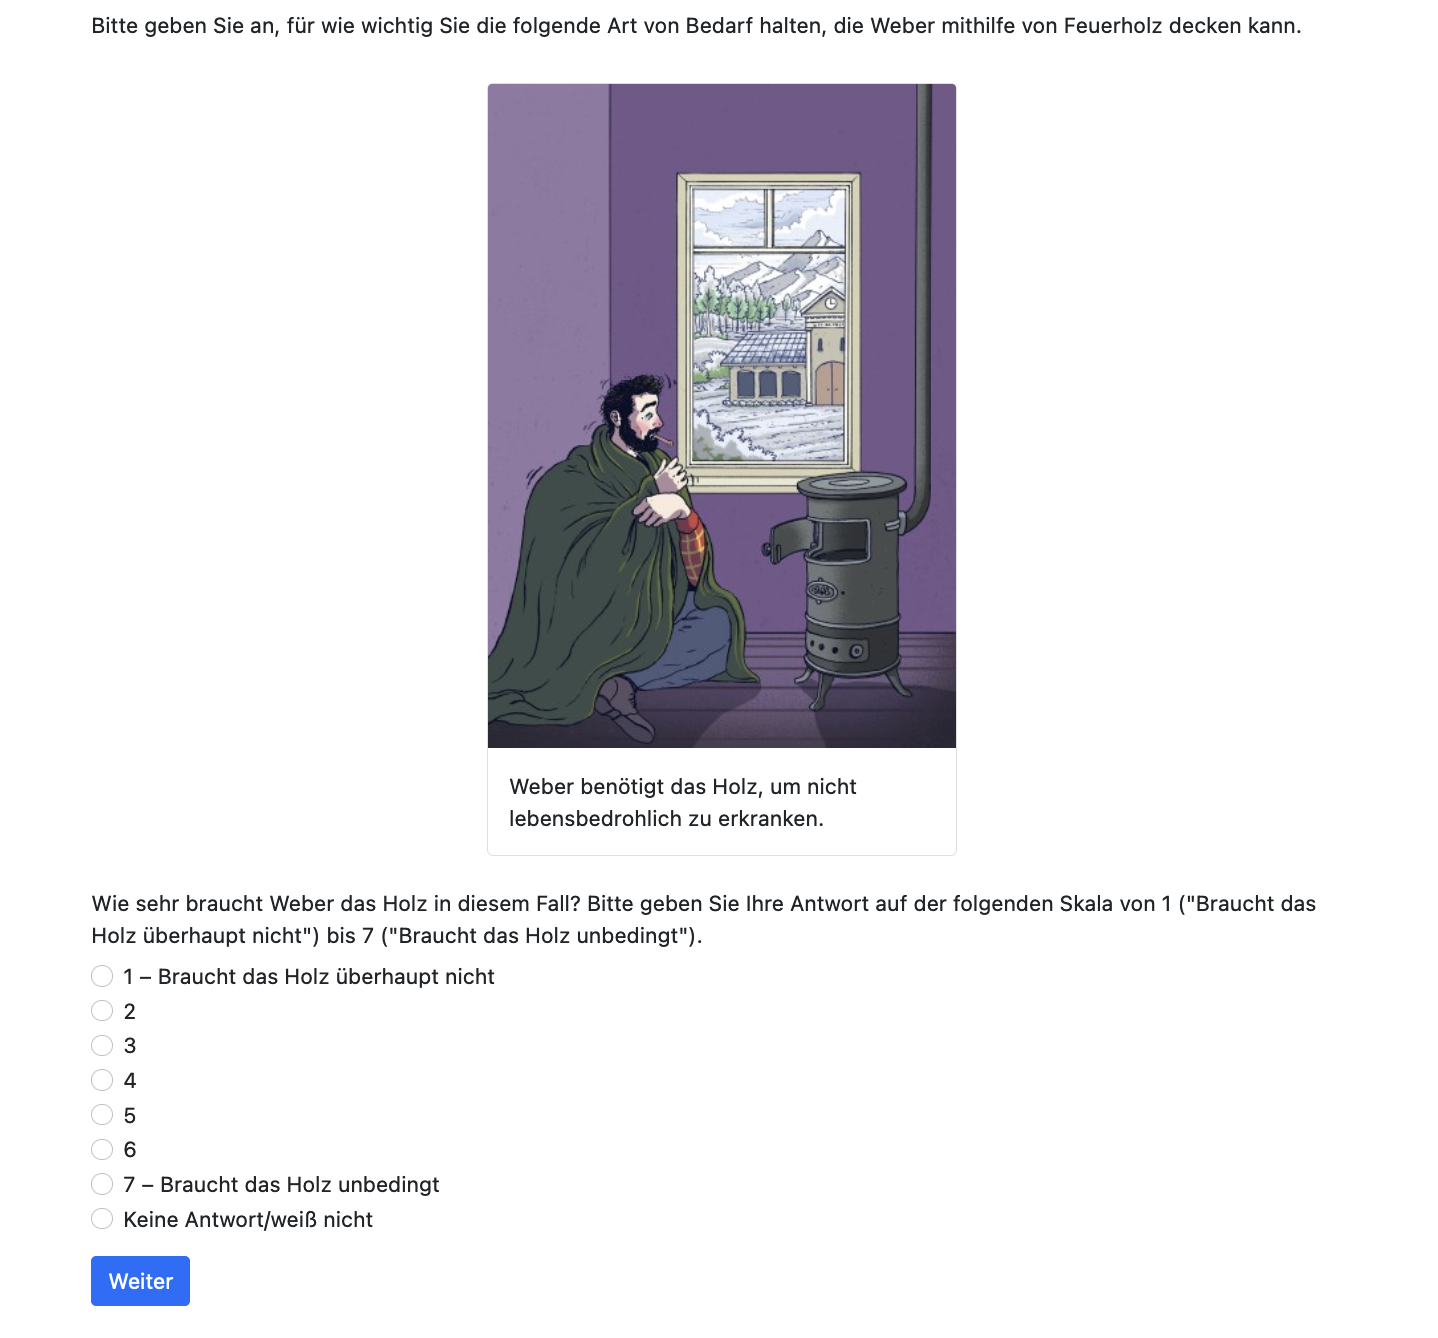
\includegraphics[width=0.4\linewidth]{figures/slides_otree_2.png}}\\
   \textcolor{gray}{Abfragebildschirm}
\end{center}
\end{frame}


%%%%%%%%%%%%
% FOLIE 44 %
%%%%%%%%%%%%
\begin{frame}{\vspace*{10mm}6.1\hspace*{1em}Studie 1}
\textbf{Ergebnisse (1/2)}\\
\medskip
\begin{center}
   \frame{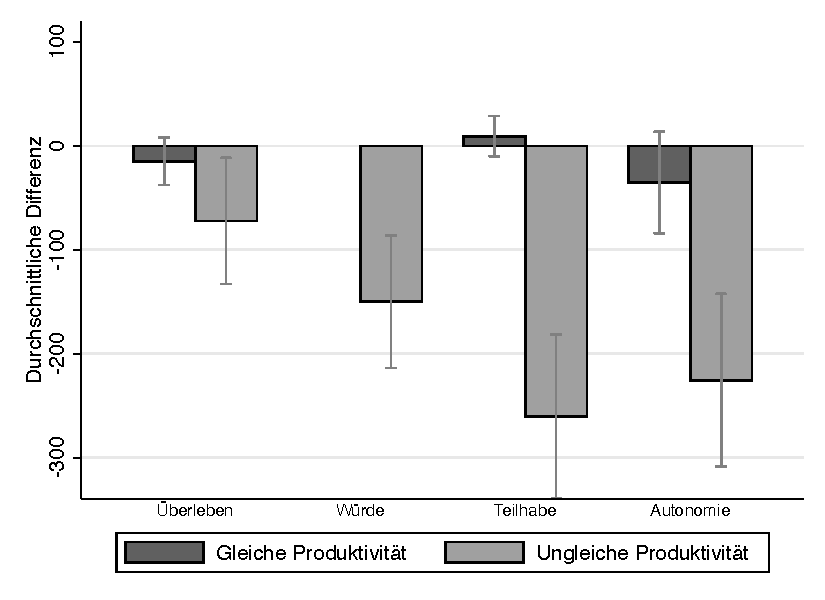
\includegraphics[width=0.5\linewidth]{figures/figure_15.pdf}}\\
   \textcolor{gray}{Einschätzung Bedeutsamkeit}
\end{center}
\end{frame}


%%%%%%%%%%%%
% FOLIE 45 %
%%%%%%%%%%%%
\begin{frame}{\vspace*{10mm}6.1\hspace*{1em}Studie 1}
\textbf{Ergebnisse (2/2)}\\
\medskip
\begin{itemize}
   \item Unparteiische Beobachter*innen schreiben verschiedenen Bedarfsarten unterschiedliche Bedeutsamkeit zu
   \item Überleben $>$ Würde $>$ Teilhabe $>$ Autonomie
\end{itemize}
\end{frame}


%%%%%%%%%%%%
% FOLIE 46 %
%%%%%%%%%%%%
\begin{frame}
\begin{overlayarea}{\textwidth}{0.81\paperheight}{
   \vspace*{11mm}
   \usebeamerfont{title}\textcolor{uolblue}
   {6.2\hspace*{1em}Studie 2}
}
\end{overlayarea}
\end{frame}


%%%%%%%%%%%%
% FOLIE 47 %
%%%%%%%%%%%%
\begin{frame}{\vspace*{10mm}6.2\hspace*{1em}Studie 2}
\textbf{Design und Durchführung (1/2)}\\
\medskip
\begin{itemize}
   \item Respondi, Online-Panel, April 2021
   \item $n=200$ (stratifiziert wie oben)
   \item Unparteiische Entscheider*innen
   \item Ermöglichungs- und Vermeidungsformulierung (\textit{between subjects})
   \item $4$ Bedarfsarten (\textit{within subjects})
   \item $14$ Verteilungsaufgaben, eingebettet in hypothetischen Kontext
\end{itemize}
\end{frame}


%%%%%%%%%%%%
% FOLIE 48 %
%%%%%%%%%%%%
\begin{frame}{\vspace*{10mm}6.2\hspace*{1em}Studie 2}
\textbf{Design und Durchführung (2/2)}\\
\medskip
\begin{center}
   \begin{tabular}{ccccccc}
      \arrayrulecolor{blue2}
      \hline
               & \multicolumn{6}{c}{Fall}                                                         \\
      Person   & 1           & 2           & 3           & 4          & 5           & 6           \\
      \hline\hline\\[-0.5em]
      A        & Überleben   & Überleben   & Überleben   & Würde      & Würde       & Teilhabe    \\
      B        & Würde       & Teilhabe    & Autonomie   & Teilhabe   & Autonomie   & Autonomie   \\
      \hline
   \end{tabular}\\
   \smallskip
   \textcolor{gray}{Zusammensetzung gemischte Fälle}
\end{center}
\end{frame}


%%%%%%%%%%%%
% FOLIE 49 %
%%%%%%%%%%%%
\begin{frame}{\vspace*{10mm}6.2\hspace*{1em}Studie 2}
\textbf{Vignette (1/6)}\\
\medskip
\enquote{Bitte stellen Sie sich zwei Personen mit den Namen $A$ und $B$ vor. $A$ und $B$ kennen sich nicht. Beide benötigen Holz. Die Gemeinde von $A$ und $B$ hat den beiden ermöglicht, in einem bestimmten Zeitraum im gemeindeeigenen Wald Holz zu schlagen. Beide verfügen über wenig Geld und haben daher keine andere Möglichkeit, sich Holz zu besorgen.\\
\medskip
Wir werden Ihnen auf den kommenden Seiten insgesamt 14 Fälle vorstellen, in denen $A$ und $B$ das Holz aus verschiedenen Gründen benötigen. Auf jeder Seite werden wir Ihnen sagen, wofür $A$ das Holz benötigt und wofür $B$ das Holz benötigt. Sie werden dann gebeten, das Holz möglichst gerecht zwischen $A$ und $B$ aufzuteilen.}
\end{frame}


%%%%%%%%%%%%
% FOLIE 50 %
%%%%%%%%%%%%
\begin{frame}{\vspace*{10mm}6.2\hspace*{1em}Studie 2}
\textbf{Vignette (2/6)}\\
\medskip
\enquote{Beachten Sie, dass Sie dabei folgende Abwägung treffen müssen: Je mehr Holz Sie einer Person geben, desto weniger können Sie der anderen Person geben. Es ist nicht möglich, die Bedarfe beider Personen gleichzeitig vollständig zu erfüllen. Die vorhandene Holzmenge würde in jedem der $14$ Fälle nur reichen, um den Bedarf einer der beiden Person gerade vollständig zu decken; die andere Person würde dann leer ausgehen.\\
\medskip
Wir stellen Ihnen nun die vier verschiedenen Gründe vor, aus denen $A$ und $B$ das Holz benötigen können. Diese vier Gründe haben mit dem kommenden Winter zu tun. Da Sie das Holz im Voraus verteilen müssen, ohne zu wissen, wie kalt der Winter genau wird, geben wir die voraussichtlichen Auswirkungen des Winters auf die Personen als mehr oder weniger wahrscheinlich an.\\
\medskip
Lesen Sie sich die Beschreibungen der vier Gründe bitte aufmerksam durch.}
\end{frame}


%%%%%%%%%%%%
% FOLIE 51 %
%%%%%%%%%%%%
\begin{frame}{\vspace*{10mm}6.2\hspace*{1em}Studie 2}
\begin{multicols}{2}
   \textbf{Vignette (3/6)}\\
   \medskip
   \enquote{Die Person benötigt das Holz, um im Winter nicht lebensbedrohlich zu erkranken und daran zu sterben. Sie heizt ihre Hütte ausschließlich mit Holz. Je mehr Holzscheite die Person bekommt, desto geringer ist die Wahrscheinlichkeit, dass sie lebensbedrohlich erkranken wird. Wenn die Person gar kein Holz bekommt, wird sie mit Sicherheit lebensbedrohlich erkranken. Wenn die Person alles verfügbare Holz bekommt, wird sie mit Sicherheit nicht lebensbedrohlich erkranken.}\\
   \vfill
   \begin{center}
      \frame{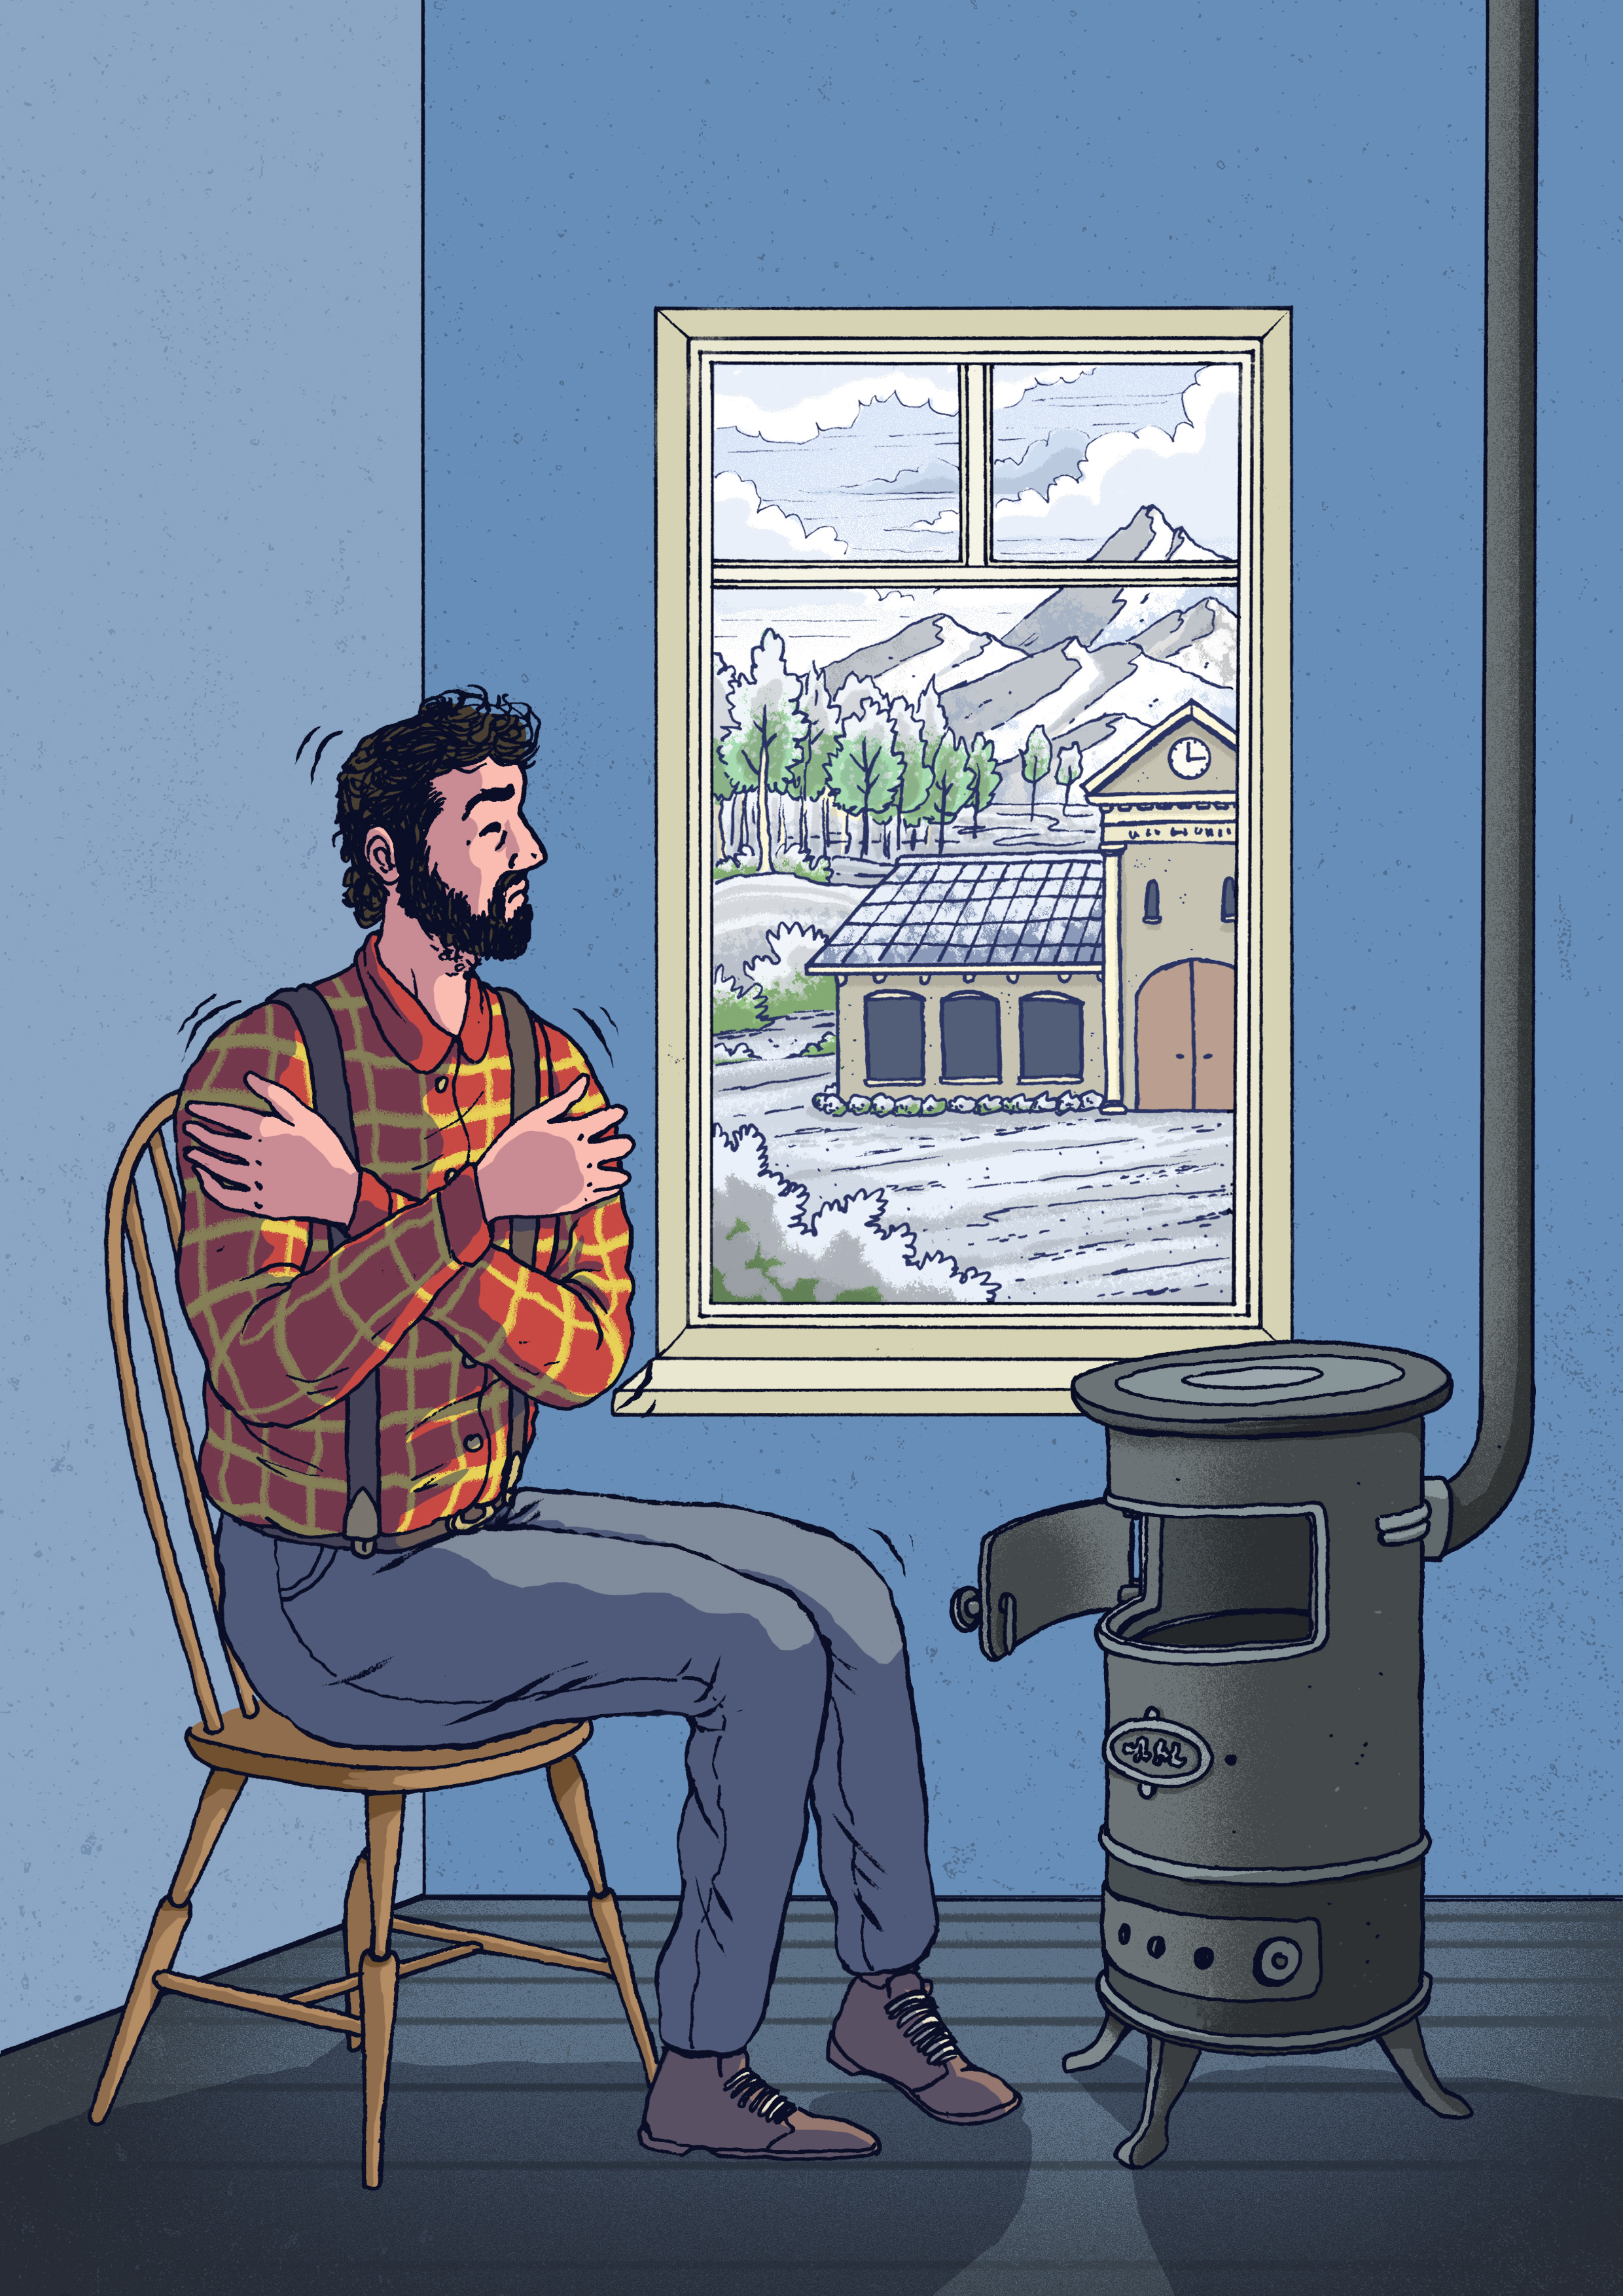
\includegraphics[width=0.6\linewidth]{figures/figure_11.jpg}}\\
      \textcolor{gray}{Illustration \textit{Überleben}}
   \end{center}
\end{multicols}
\end{frame}


%%%%%%%%%%%%
% FOLIE 52 %
%%%%%%%%%%%%
\begin{frame}{\vspace*{10mm}6.2\hspace*{1em}Studie 2}
\begin{multicols}{2}
   \textbf{Vignette (4/6)}\\
   \medskip
   \enquote{Die Person benötigt das Holz, um im Winter nicht zu frieren. Sie heizt ihre Hütte ausschließlich mit Holz. Je mehr Holzscheite die Person bekommt, desto geringer ist die Wahrscheinlichkeit, dass sie frieren wird. Wenn die Person gar kein Holz bekommt, wird sie mit Sicherheit frieren. Wenn die Person alles verfügbare Holz bekommt, wird sie mit Sicherheit nicht frieren.}\\
   \vfill
   \begin{center}
      \frame{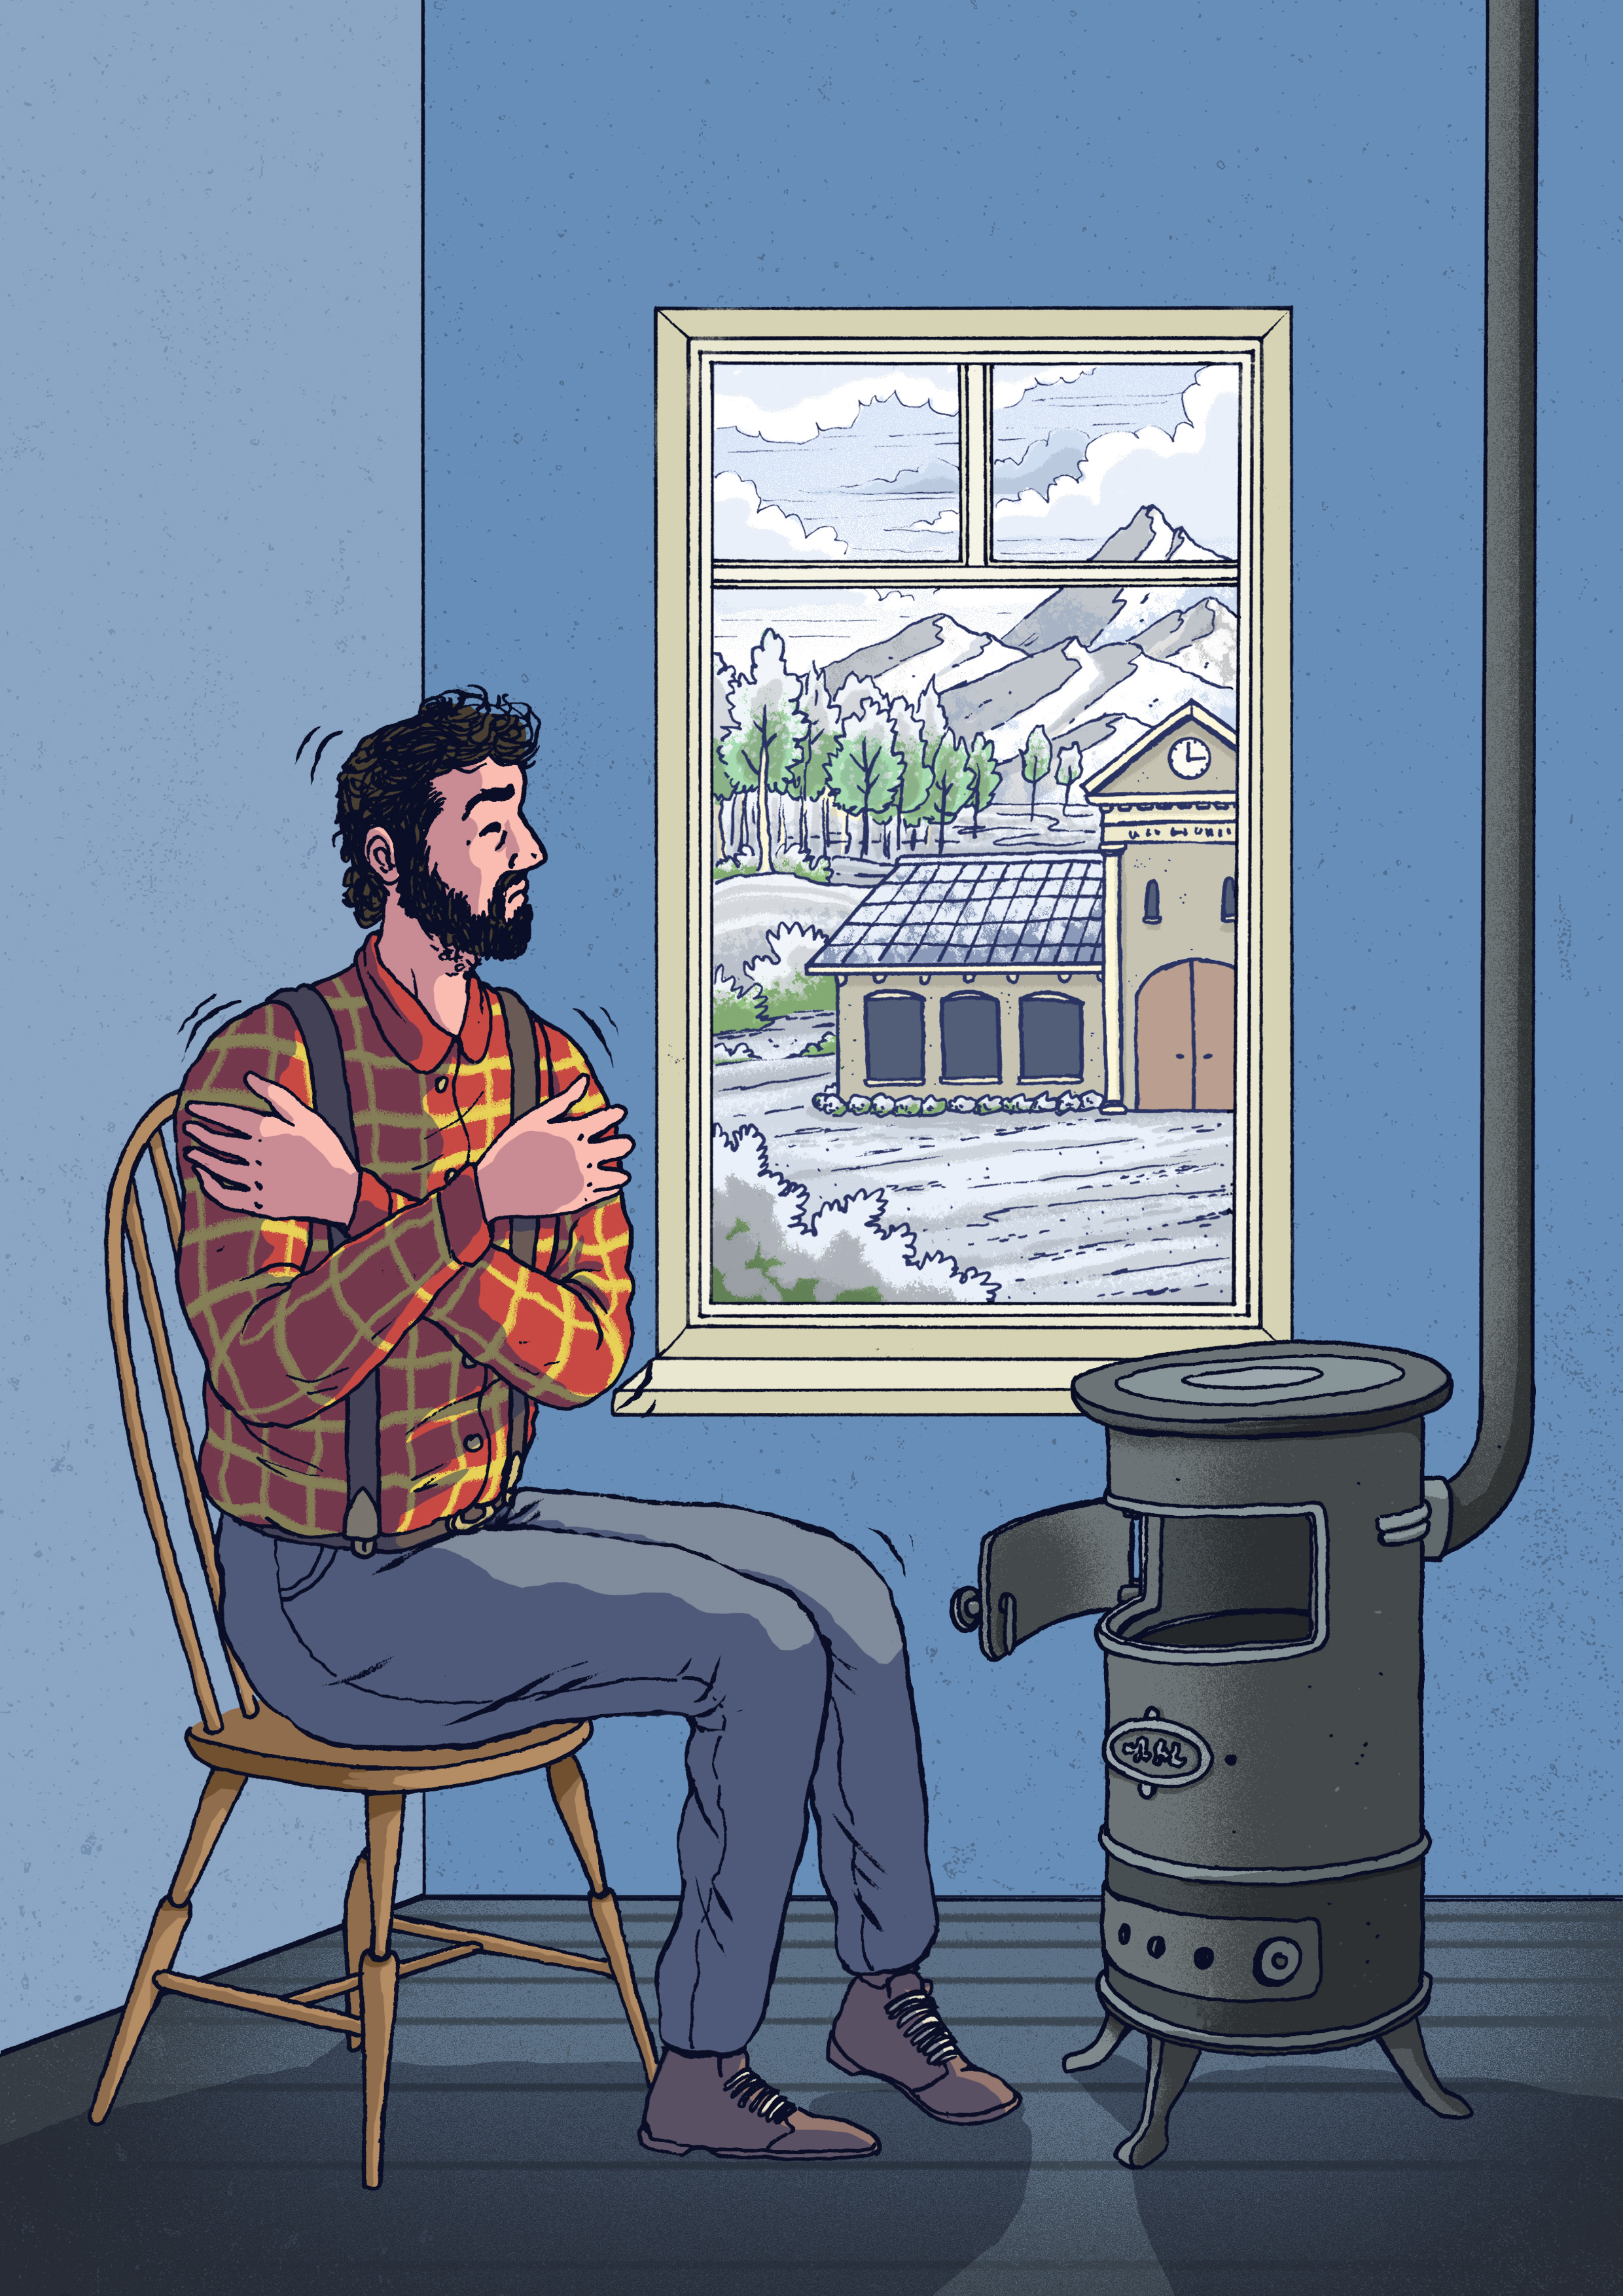
\includegraphics[width=0.6\linewidth]{figures/figure_12.jpg}}\\
      \textcolor{gray}{Illustration \textit{Würde}}
   \end{center}
\end{multicols}
\end{frame}


%%%%%%%%%%%%
% FOLIE 53 %
%%%%%%%%%%%%
\begin{frame}{\vspace*{10mm}6.2\hspace*{1em}Studie 2}
\begin{multicols}{2}
   \textbf{Vignette (5/6)}\\
   \medskip
   \enquote{Die Person benötigt das Holz, um im Winter nicht vom sozialen Leben ausgeschlossen zu sein, da es Gang und Gäbe ist, dass man sich im Gemeindehaus trifft und jeder Holz mitbringt, mit dem das Gemeindehaus beheizt werden kann. Je mehr Holzscheite die Person bekommt, desto geringer ist die Wahrscheinlichkeit, dass sie vom sozialen Leben ausgeschlossen sein wird. Wenn die Person gar kein Holz bekommt, wird sie mit Sicherheit vom sozialen Leben ausgeschlossen sein. Wenn die Person alles verfügbare Holz bekommt, wird sie mit Sicherheit nicht vom sozialen Leben ausgeschlossen sein.}\\
   \vfill
   \begin{center}
      \frame{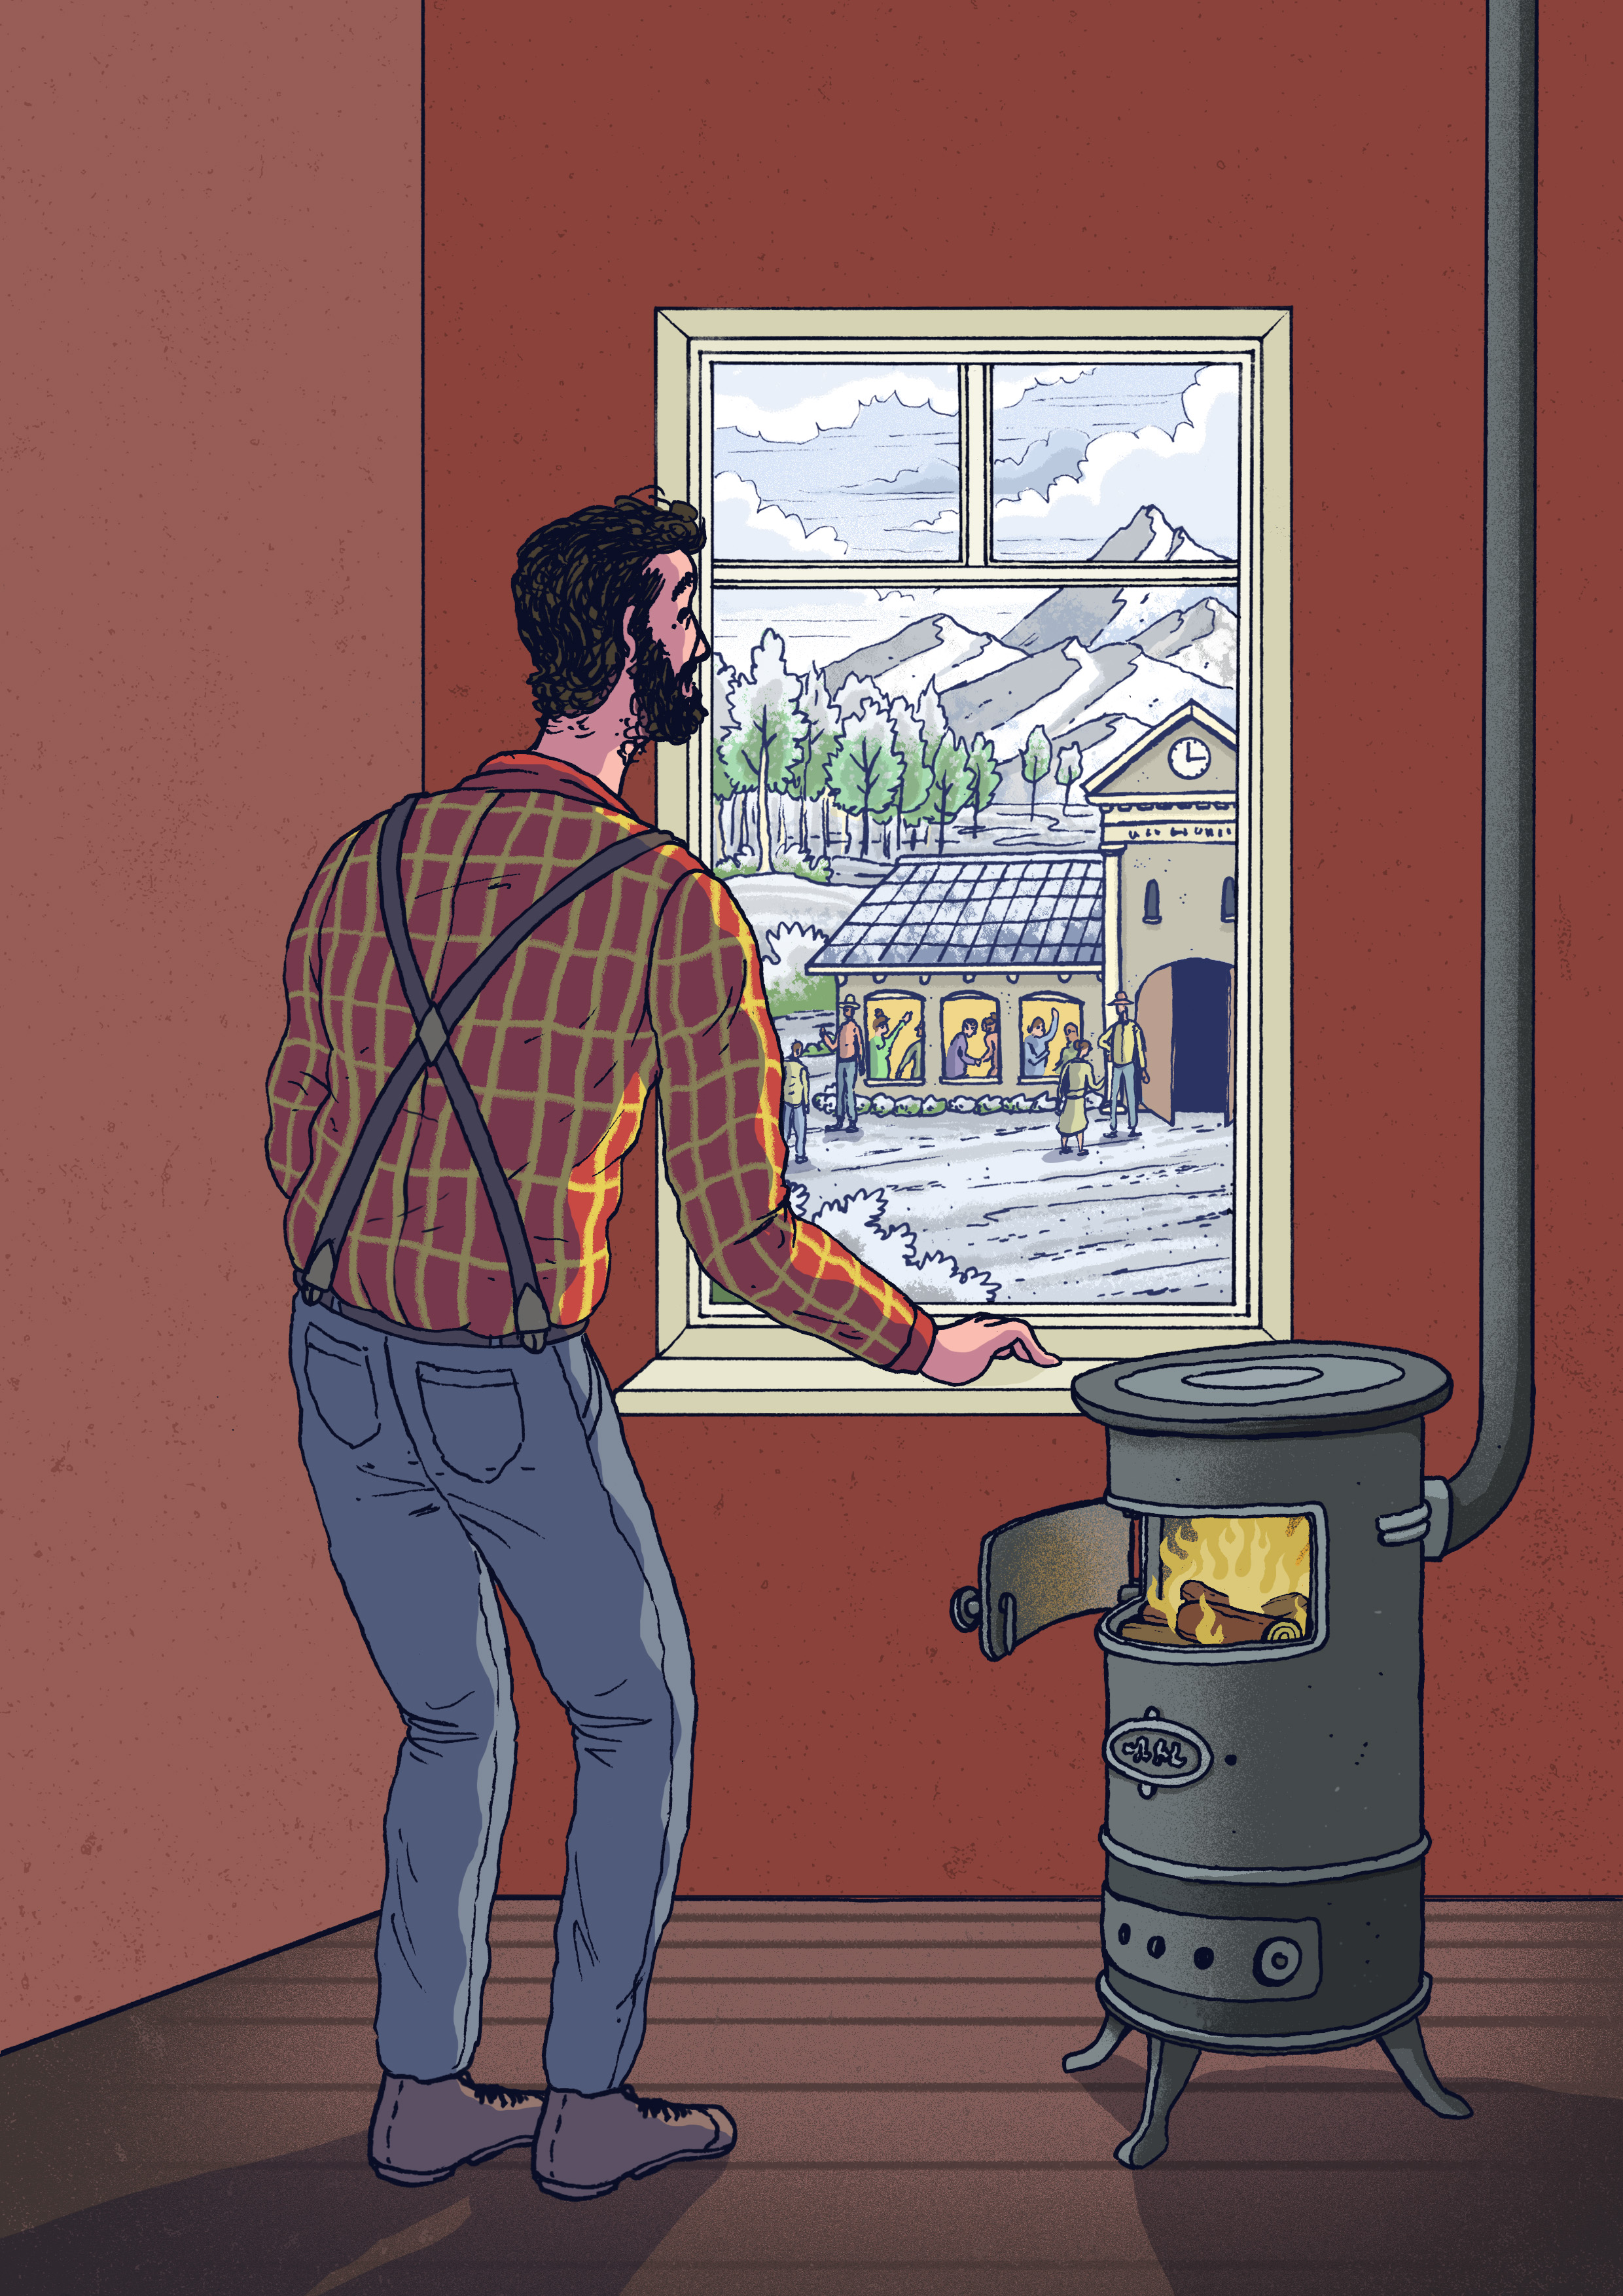
\includegraphics[width=0.6\linewidth]{figures/figure_13.jpg}}\\
      \textcolor{gray}{Illustration \textit{Teilhabe}}
   \end{center}
\end{multicols}
\end{frame}


%%%%%%%%%%%%
% FOLIE 54 %
%%%%%%%%%%%%
\begin{frame}{\vspace*{10mm}6.2\hspace*{1em}Studie 2}
\begin{multicols}{2}
   \textbf{Vignette (6/6)}\\
   \medskip
   \enquote{Die Person benötigt das Holz, damit ihr Atelier im Winter nicht unbenutzbar wird. Sie heizt ihr Atelier ausschließlich mit Holz. Dort schafft sie in ihrer Freizeit Kunst. Je mehr Holzscheite die Person bekommt, desto geringer ist die Wahrscheinlichkeit, dass ihr Atelier unbenutzbar wird. Wenn die Person gar kein Holz bekommt, wird ihr Atelier mit Sicherheit unbenutzbar sein. Wenn die Person alles verfügbare Holz bekommt, wird ihr Atelier mit Sicherheit nicht unbenutzbar sein.}\\
   \vfill
   \begin{center}
      \frame{
\includegraphics[width=0.6\linewidth]{figures/figure_14.jpg}}\\
      \textcolor{gray}{Illustration \textit{Autonomie}}
   \end{center}
\end{multicols}
\end{frame}


%%%%%%%%%%%%
% FOLIE 55 %
%%%%%%%%%%%%
\begin{frame}{\vspace*{10mm}6.2\hspace*{1em}Studie 2}
\textbf{Abfrage}\\
\medskip
\begin{center}
   \frame{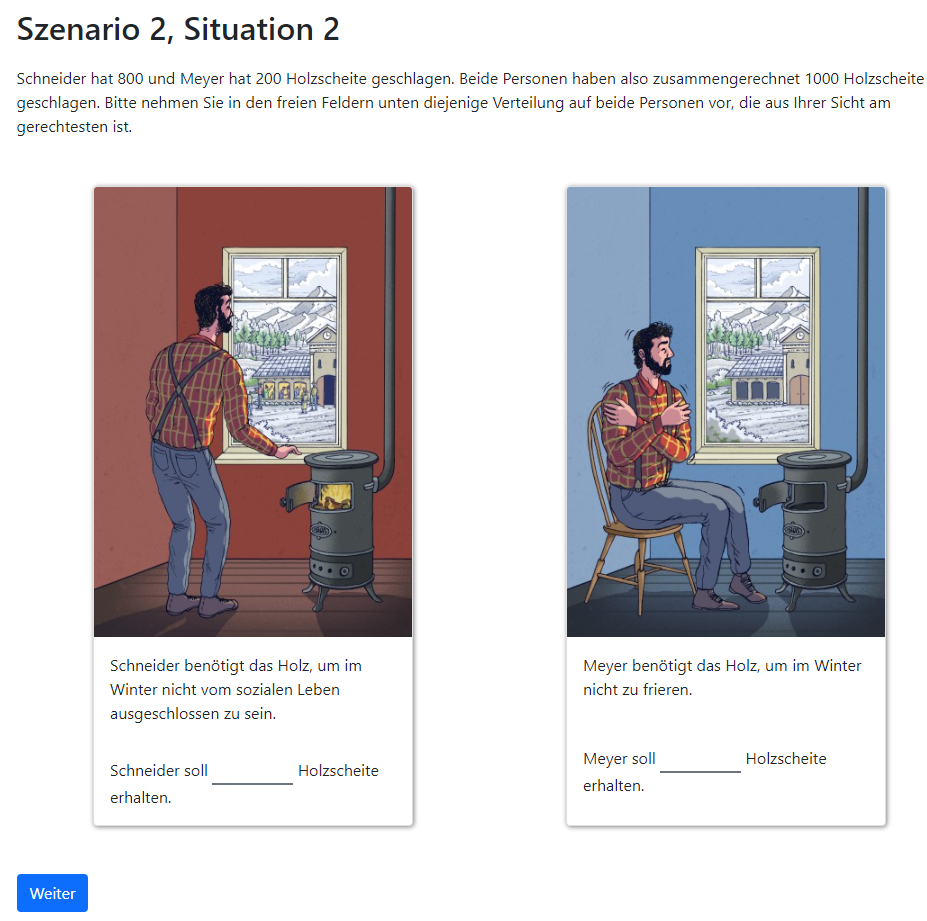
\includegraphics[width=0.4\linewidth]{figures/slides_otree_3.png}}\\
   \textcolor{gray}{Abfragebildschirm}
\end{center}
\end{frame}


%%%%%%%%%%%%
% FOLIE 56 %
%%%%%%%%%%%%
\begin{frame}{\vspace*{10mm}6.2\hspace*{1em}Studie 2}
\textbf{Ergebnisse (1/4)}\\
\medskip
\begin{center}
   \frame{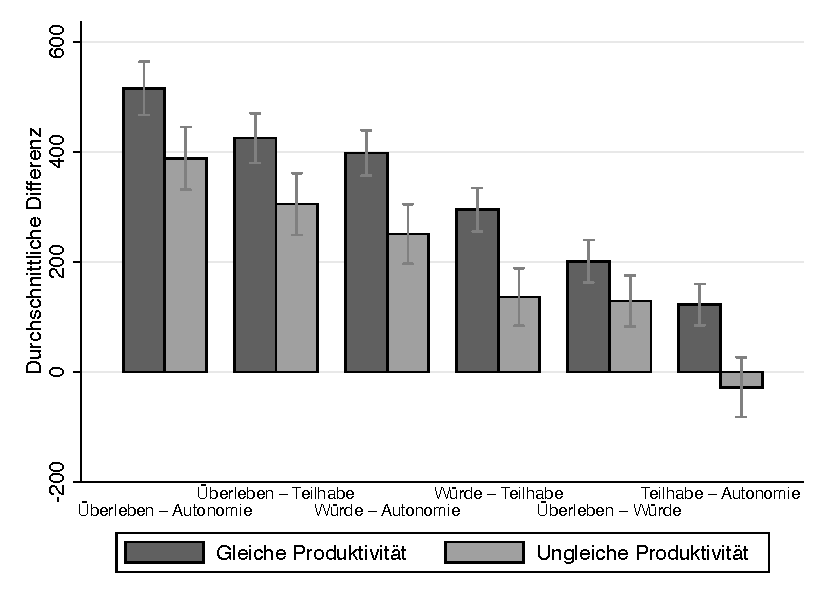
\includegraphics[width=0.5\linewidth]{figures/figure_16.pdf}}\\
   \textcolor{gray}{Differenz gepaarte Fälle}
\end{center}
\end{frame}


%%%%%%%%%%%%
% FOLIE 57 %
%%%%%%%%%%%%
\begin{frame}{\vspace*{10mm}6.2\hspace*{1em}Studie 2}
\textbf{Ergebnisse (2/4)}\\
\medskip
\begin{center}
   \frame{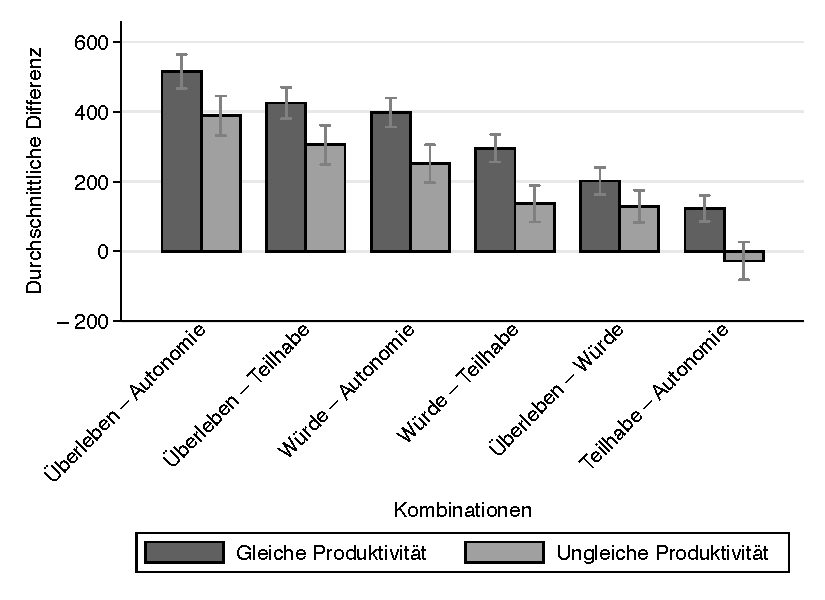
\includegraphics[width=0.5\linewidth]{figures/figure_17.pdf}}\\
   \textcolor{gray}{Differenz gemischte Fälle}
\end{center}
\end{frame}


%%%%%%%%%%%%
% FOLIE 58 %
%%%%%%%%%%%%
\begin{frame}{\vspace*{10mm}6.2\hspace*{1em}Studie 2}
\textbf{Ergebnisse (3/4)}\\
\medskip
\begin{center}
   \frame{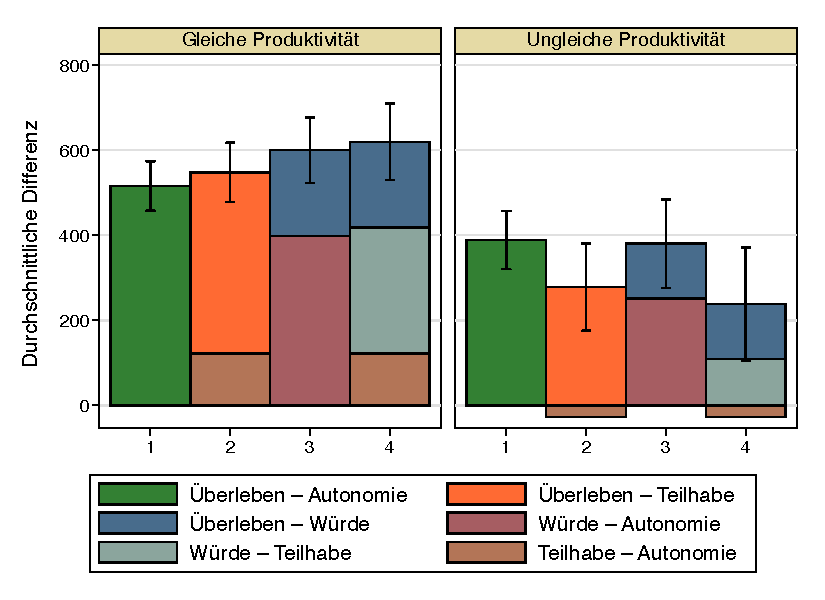
\includegraphics[width=0.5\linewidth]{figures/figure_18.pdf}}\\
   \textcolor{gray}{Additivität}
\end{center}
\end{frame}


%%%%%%%%%%%%
% FOLIE 59 %
%%%%%%%%%%%%
\begin{frame}{\vspace*{10mm}6.2\hspace*{1em}Studie 2}
\textbf{Ergebnisse (4/4)}\\
\medskip
\begin{itemize}
   \item \textcolor{gray}{Unparteiische} Entscheider*innen \textcolor{gray}{schreiben verschiedenen Bedarfsarten unterschiedliche Bedeutsamkeit zu}
   \item \textcolor{gray}{Überleben $>$ Würde $>$ Teilhabe $>$ Autonomie}
   \item Durchschnittliche Differenzen der Verteilungsentscheidungen sind kohärent
\end{itemize}
\end{frame}


%%%%%%%%%%%%
% FOLIE 60 %
%%%%%%%%%%%%
\begin{frame}
\begin{overlayarea}{\textwidth}{0.81\paperheight}{
   \vspace*{11mm}
   \usebeamerfont{title}\textcolor{uolblue}
   {7\hspace*{1em}Zusammenfassung\\\hspace*{1.5em}zentraler Ergebnisse}
}
\end{overlayarea}
\end{frame}


%%%%%%%%%%%%
% FOLIE 61 %
%%%%%%%%%%%%
\begin{frame}{\vspace*{10mm}7\hspace*{1em}Zusammenfassung zentraler Ergebnisse}
\begin{multicols}{2}
   \textbf{Bedarf als Referenzpunkt}
   \medskip
   \begin{itemize}
   \item[(1)] Unparteiische Beobachter*innen nehmen graduelle Gerechtigkeitseinschätzungen vor
   \item[(2)] Diese Einschätzungen sind abhängig von Versorgungssituationen
   \item[(3)] Bedarfsinformationen beeinflussen diese Einschätzungen
\end{itemize}
   \vfill
   \begin{center}
      \frame{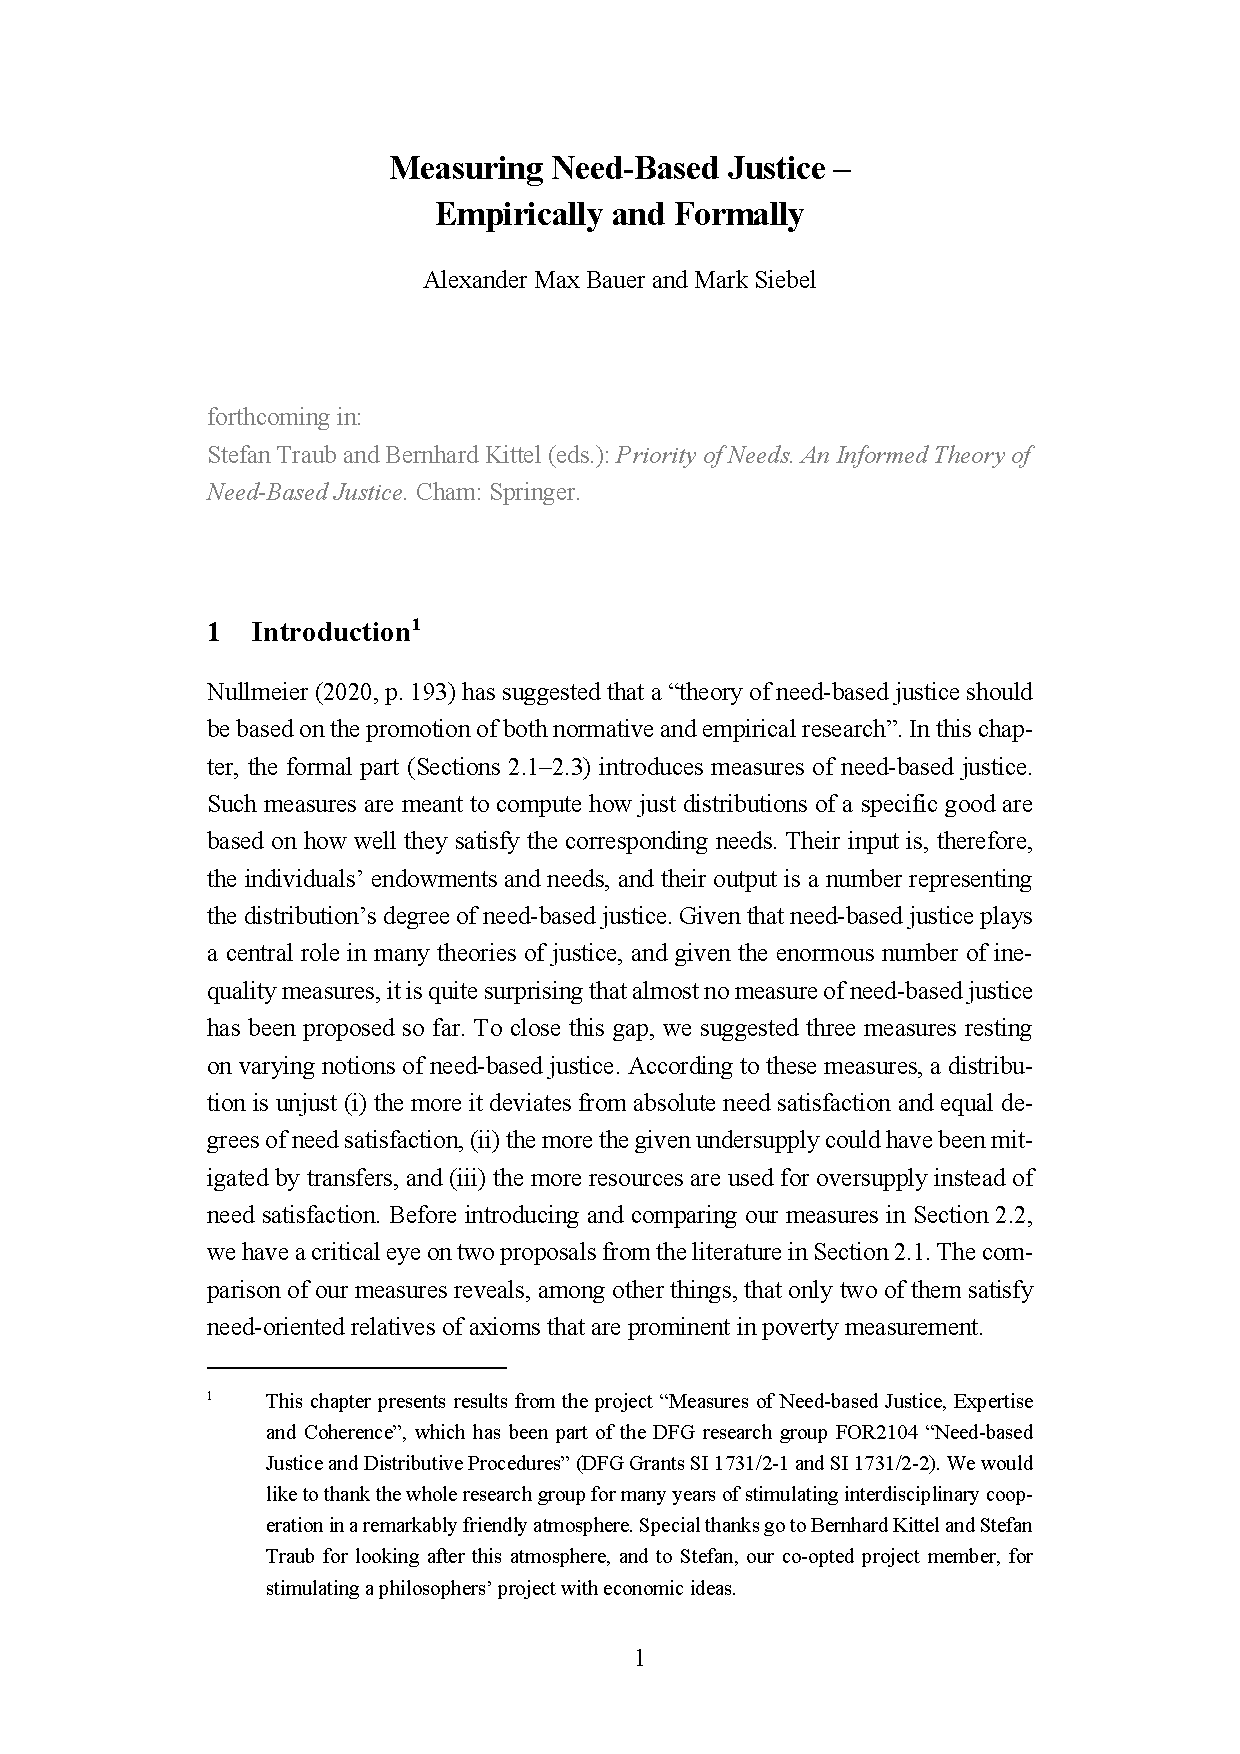
\includegraphics[width=0.6\linewidth]{figures/slides_bauer_siebel_nd.pdf}}\\
      \textcolor{gray}{Bauer und Siebel i.\,V.}
   \end{center}
\end{multicols}
\end{frame}


%%%%%%%%%%%%
% FOLIE 62 %
%%%%%%%%%%%%
\begin{frame}{\vspace*{10mm}7\hspace*{1em}Zusammenfassung zentraler Ergebnisse}
\textbf{Bedarf und Verantwortung}\\
\medskip
\begin{itemize}
   \item[(4)] Unparteiische Entscheider*innen berücksichtigen Bedarf, Leistung und Verantwortung
   \item[(5)] Auch bei zu geringer Leistung wird Bedarf teilweise kompensiert
   \item[(6)] Kompensationsbereitschaft sinkt, wenn zu geringe Leistung selbst verschuldet ist
\end{itemize}
\vspace{2em}
\textbf{Bedarfsarten}\\
\medskip
\begin{itemize}
   \item[(7)] Unparteiische Beobachter*innen und Entscheider*innen unterscheiden Bedarfsarten
   \end{itemize}
\end{frame}


%%%%%%%%%%%%
% FOLIE 63 %
%%%%%%%%%%%%
\begin{frame}{}
\begin{center}
   
\includegraphics[width=0.8\linewidth]{figures/slides_thanks.pdf}
\end{center}
\end{frame}


%%%%%%%%%%%%
% FOLIE 64 %
%%%%%%%%%%%%
\begin{frame}{\vspace*{10mm}Bibliografie}
\vspace*{-10mm}
{\footnotesize
\begin{itemize}[label=,leftmargin=2em,itemindent=-2em]
   \item Aristoteles (2011): \textit{Nikomachische Ethik}. Hrsg. von Ursula Wolf. Hamburg: Rowohlt.
   \item Bauer, Alexander Max (2019): \enquote{Gerechtigkeit und Bedürfnis. Perspektiven auf den Begriff des \enquote{Bedürfnisses} vor dem Hintergrund der Bedarfsgerechtigkeit}. In: Alexander Max Bauer und Nils Baratella (Hrsg.): \textit{Oldenburger Jahrbuch für Philosophie 2017/2018}. Oldenburg: BIS-Verlag. S. 285--327.
   \item Bauer, Alexander Max, Adele Diederich, Stefan Traub und Arne Robert Weiss (2023): \enquote{When the Poorest Are Neglected. A Vignette Experiment on Need-Based Distributive Justice}. \textit{SSRN Working Paper} 4503209.
   \item Bauer, Alexander Max, Frauke Meyer, Jan Romann, Mark Siebel und Stefan Traub (2022): \enquote{Need, Equity, and Accountability. Evidence on Third-Party Distributive Decisions from a Vignette Study}. In: \textit{Social Choice and Welfare} 59, S. 769--814.
   \item Bauer, Alexander Max und Malte Ingo Meyerhuber (2019): \enquote{Zwei Welten am Rande der Kollision. Zum Verhältnis von empirischer Forschung und normativer Theorie, insbesondere vor dem Hintergrund der Ethik}. In: dies. (Hrsg.): \textit{Philosophie zwischen Sein und Sollen. Normative Theorie und empirische Forschung im Spannungsfeld}. Berlin und Boston: Walter de Gruyter. S. 13--37.
\end{itemize}
}
\end{frame}


%%%%%%%%%%%%
% FOLIE 65 %
%%%%%%%%%%%%
\begin{frame}{\vspace*{10mm}Bibliografie}
\vspace*{-10mm}
{\footnotesize
\begin{itemize}[label=,leftmargin=2em,itemindent=-2em]
   \item Bauer, Alexander Max und Jan Romann (i.\,V.): \enquote{Equal Deeds, Different Needs. Need, Accountability, and Ressource Availability in Third-Party Distributive Decisions}. In: Shaun Nichols und Joshua Knobe (Hrsg.): \textit{Oxford Studies in Experimental Philosophy}. Oxford: Oxford University Press.
   \item Bauer, Alexander Max, Jan Romann, Mark Siebel und Stefan Traub (2023): \enquote{Winter is Coming. How Laypeople Think About Different Kinds of Needs}. \textit{PLoS ONE} 18 (11), e0294572.
   \item Bauer, Alexander Max und Mark Siebel (i.\,V.): \enquote{Measuring Need-Based Distributive Justice -- Formally and Empirically}. In: Stefan Traub und Bernhard Kittel (Hrsg.): \textit{Priority of Needs. An Informed Theory of Need-Based Justice}. Cham: Springer.
   \item Platon (2004): \enquote{Der Staat}. In: ders.: \textit{Sämtliche Werke in drei Bänden}. Bd. 2. Hrsg. von Erich Loewenthal. Übers. von Wilhelm Sigismund Teuffel und Wilhelm Wiegand. Darmstadt: Wissenschaftliche Buchgesellschaft. S. 5--407.
   \item Sen, Amartya (2012): \textit{Die Idee der Gerechtigkeit}. München: Deutscher Taschenbuch Verlag.
\end{itemize}
}
\end{frame}


%%%%%%%%%%%%
% FOLIE 66 %
%%%%%%%%%%%%
\begin{frame}
\begin{overlayarea}{\textwidth}{0.81\paperheight}{
   \vspace*{11mm}
   \usebeamerfont{title}\textcolor{uolblue}
   {Zusätzliche Folien}
}
\end{overlayarea}
\end{frame}


%%%%%%%%%%%%
% FOLIE 67 %
%%%%%%%%%%%%
\begin{frame}{\vspace*{10mm}2\hspace*{1em}Empirische Forschung und normative Theorie}
\begin{center}
   \frame{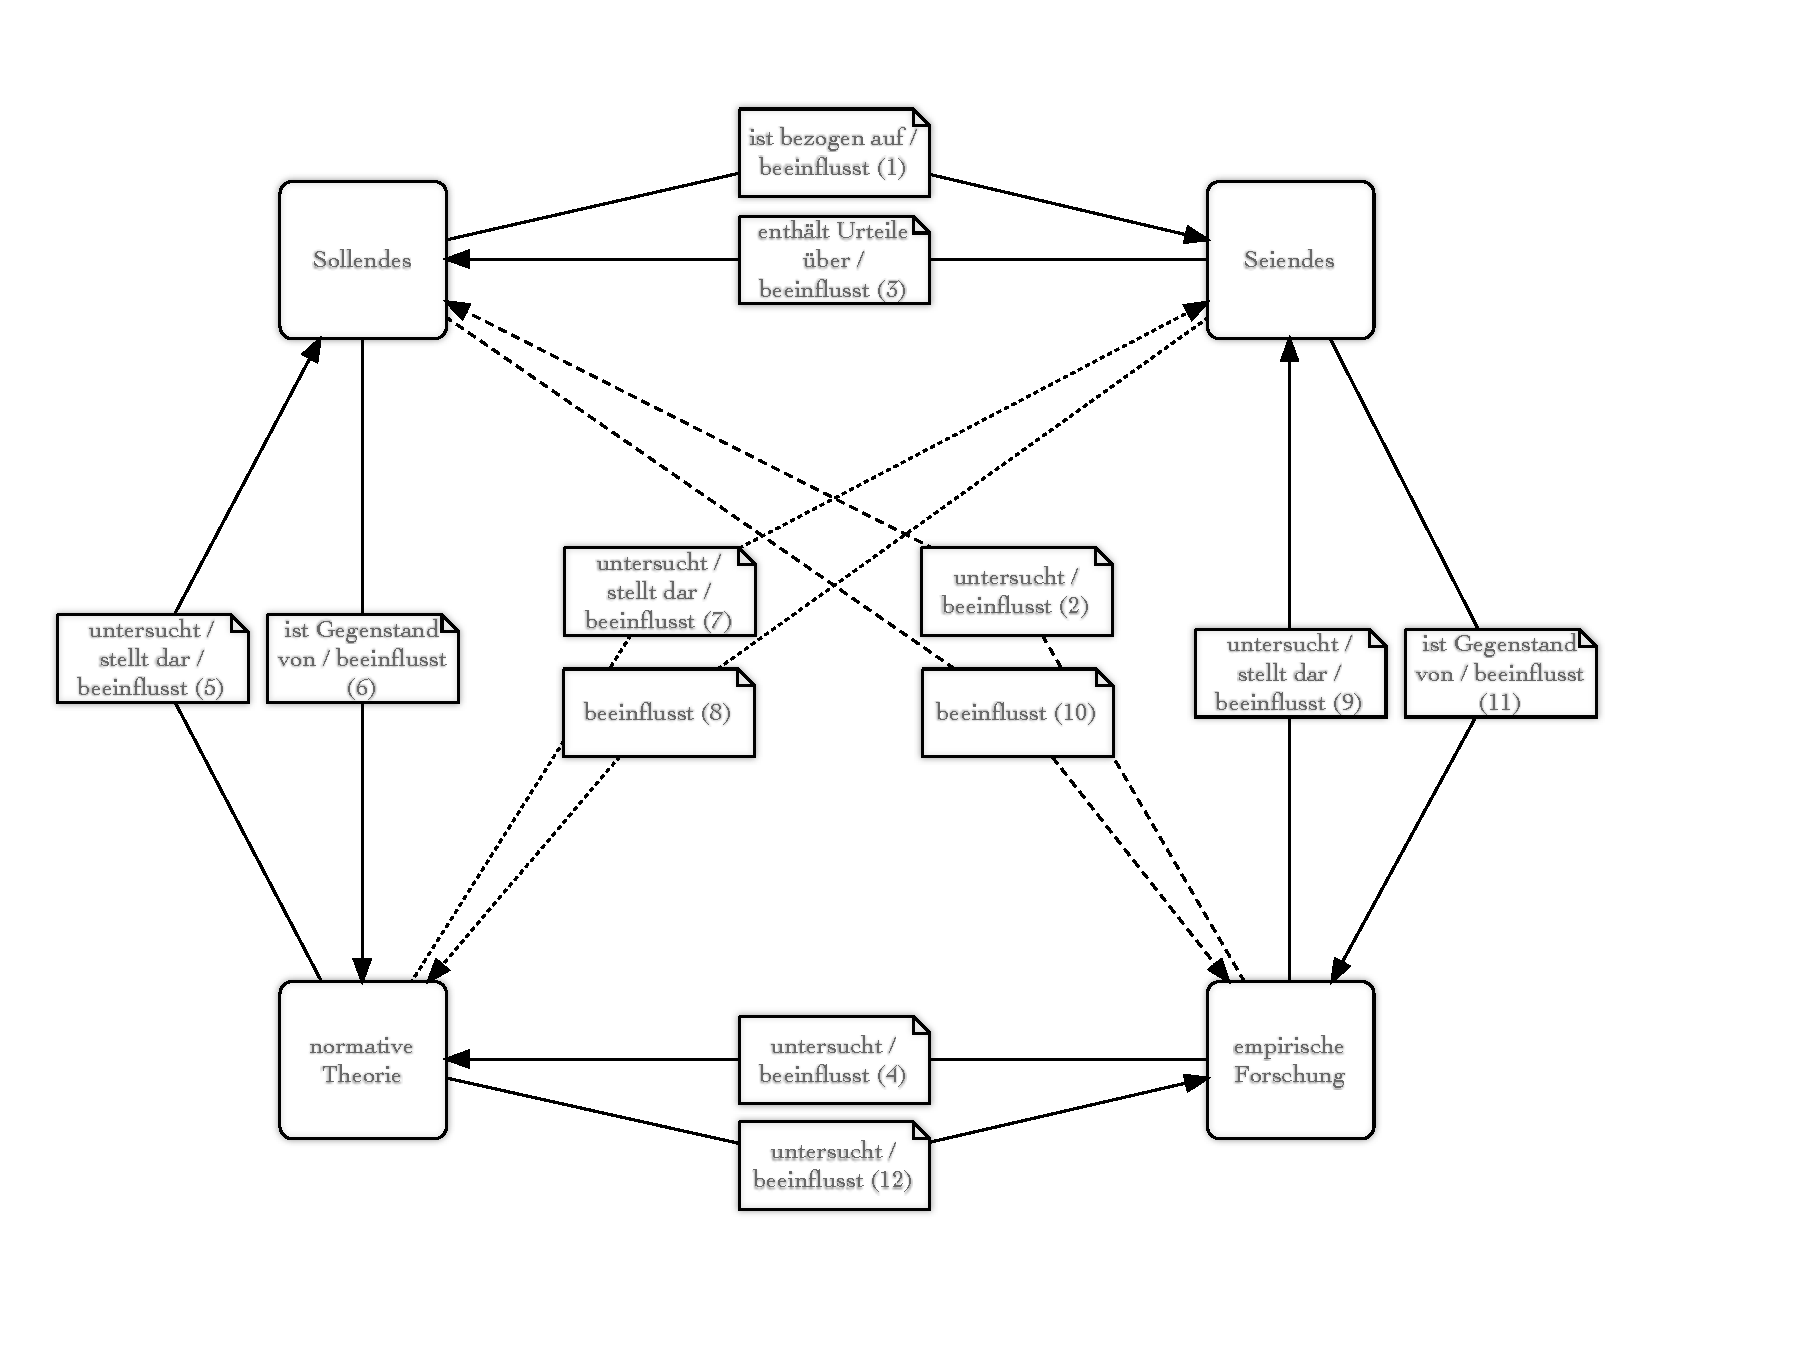
\includegraphics[width=0.6\linewidth]{figures/slides_emp_norm.pdf}}\\
   \textcolor{gray}{Beziehungsgeflecht}
\end{center}
\end{frame}


%%%%%%%%%%%%
% FOLIE 68 %
%%%%%%%%%%%%
\begin{frame}{\vspace*{10mm}3\hspace*{1em}Bedarf und Bedarfsgerechtigkeit}
\begin{center}
   \frame{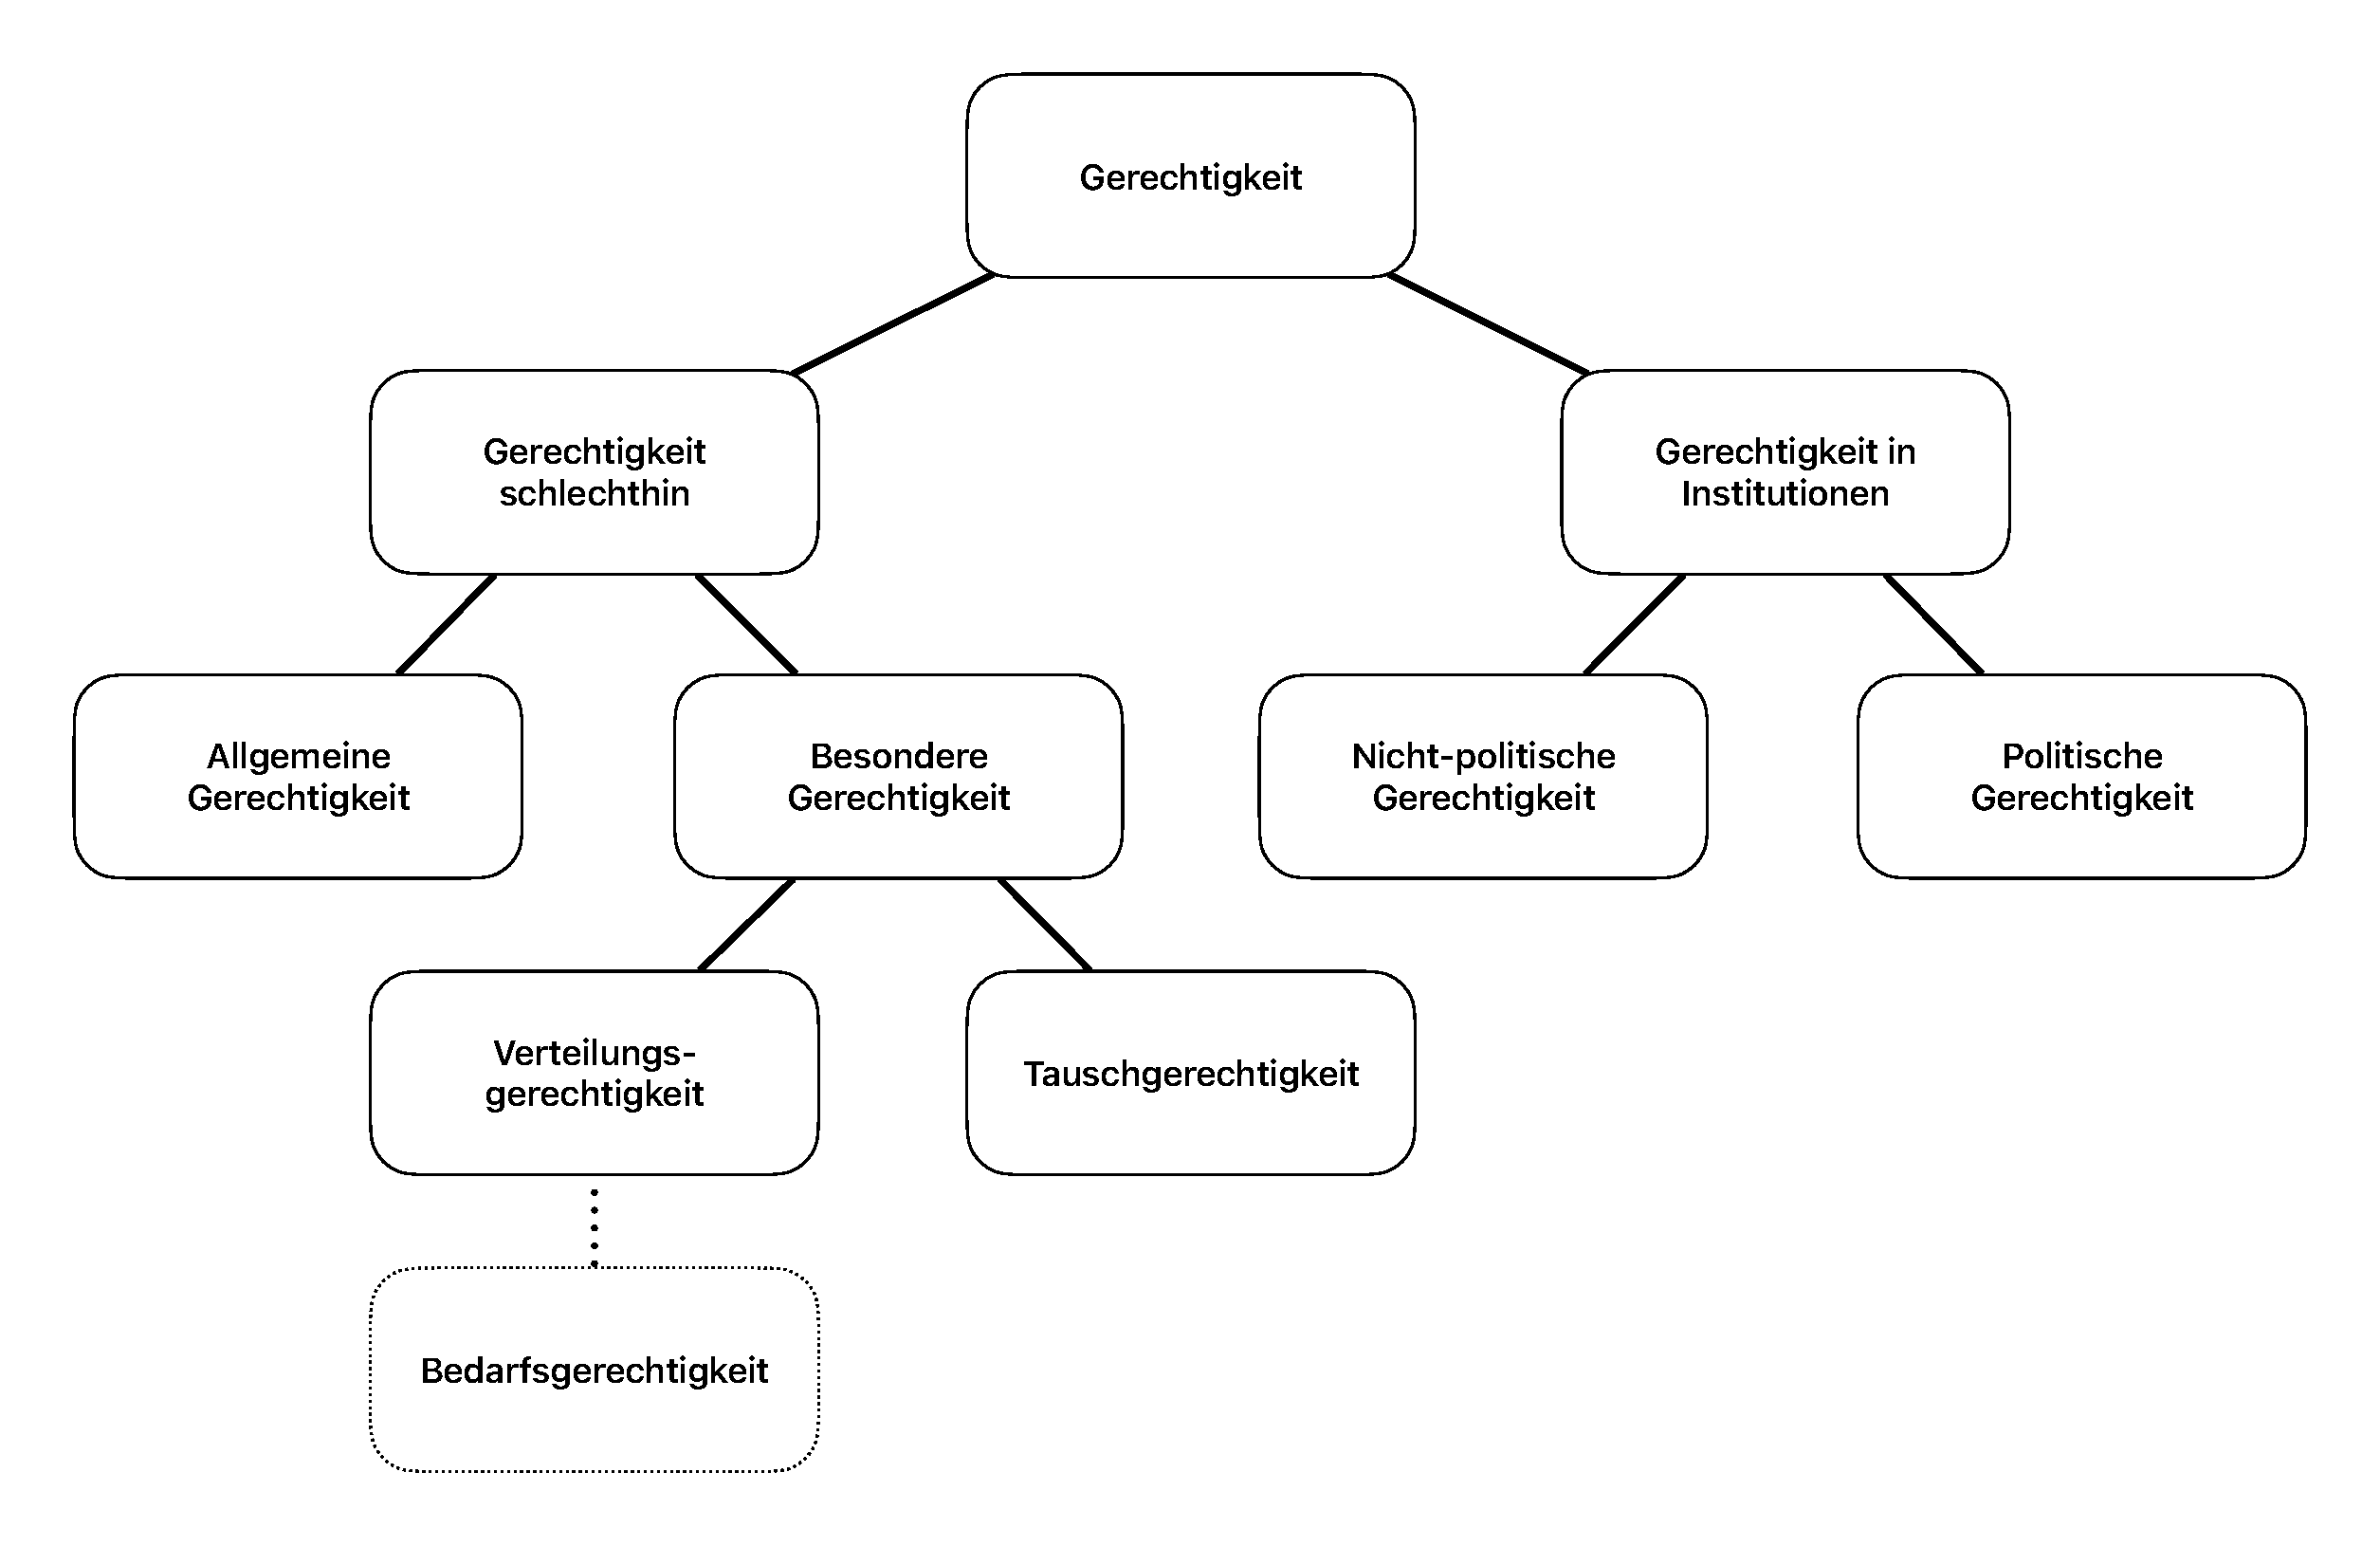
\includegraphics[width=0.6\linewidth]{figures/slides_justice.pdf}}\\
   \textcolor{gray}{Typisierung der Gerechtigkeit nach Aristoteles}
\end{center}
\end{frame}


%%%%%%%%%%%%
% FOLIE 69 %
%%%%%%%%%%%%
\begin{frame}{\vspace*{10mm}4\hspace*{1em}Bedarf als Referenzpunkt}
\begin{multicols}{2}
   \begin{center}
      \frame{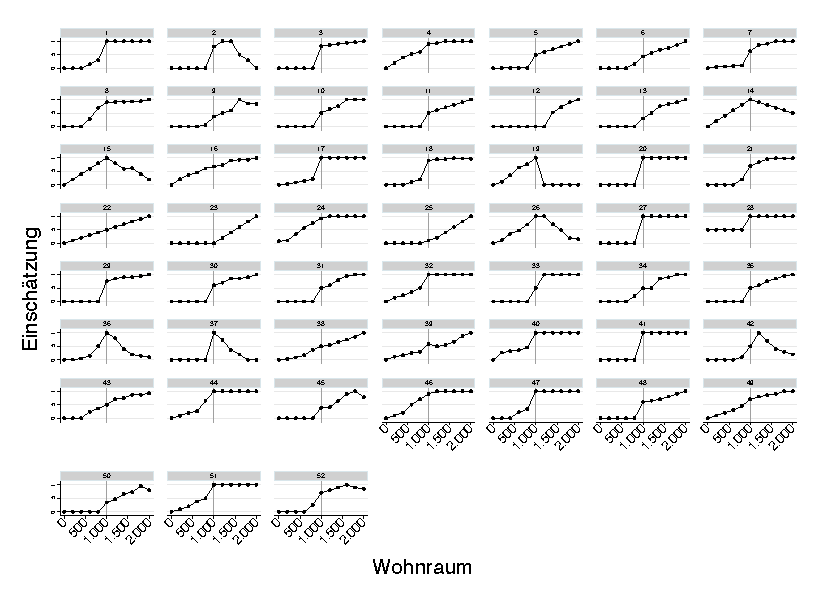
\includegraphics[width=1\linewidth]{figures/figure_3.pdf}}\\
      \textcolor{gray}{Individuelle Einschätzungen Bedarfsgruppe}
      \frame{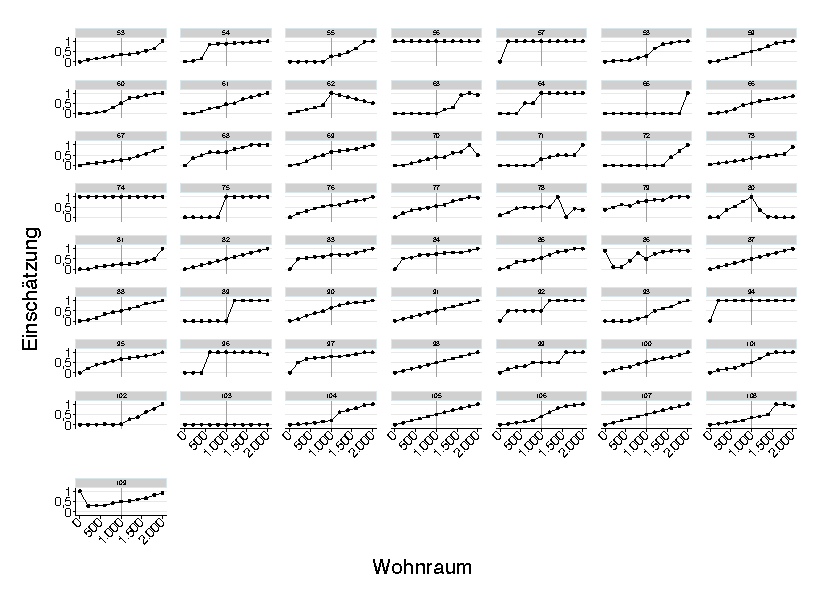
\includegraphics[width=1\linewidth]{figures/figure_4.pdf}}\\
      \textcolor{gray}{Individuelle Einschätzungen Kontrollgruppe}
   \end{center}
\end{multicols}
\end{frame}


%%%%%%%%%%%%
% FOLIE 70 %
%%%%%%%%%%%%
\begin{frame}{\vspace*{10mm}4\hspace*{1em}Bedarf als Referenzpunkt}
\begin{center}
   \begin{tabular}[h]{lrrrrrrl}
      \arrayrulecolor{blue2}
      \hline
      Typ              & \multicolumn{5}{c}{Häufigkeit}      &   & Prinzip                                                              \\
      \cline{2-6}
                       & \multicolumn{2}{c}{Bedarfsgruppe}   &   & \multicolumn{2}{c}{Kontrollgruppe}   &   &                           \\
      \hline\hline\\[-0.5em]
      Hügelförmig      &  8   &  (15,38\,\%)                 &   &  2   &   (3,51\,\%)                  &   & \enquote{Strikter}        \\
                       &      &                              &   &      &                               &   & Suffizientarismus         \\[1ex]
      Binär            &  4   &   (7,69\,\%)                 &   &  5   &   (8,77\,\%)                  &   & \enquote{Qualitativer}    \\
                       &      &                              &   &      &                               &   & Suffizientarismus         \\[1ex]
      Flach ab         &  7   &  (13,46\,\%)                 &   &  1   &   (1,75\,\%)                  &   & \enquote{Quantitativer}   \\
      der Schwelle     &      &                              &   &      &                               &   & Suffizientarismus         \\[1ex]
      Null unterhalb   & 15   &  (28,85\,\%)                 &   &  5   &   (8,77\,\%)                  &   & \enquote{Strikter}        \\
      der Schwelle     &      &                              &   &      &                               &   & Prioritarismus            \\[1ex]
      Ansteigend       & 17   &  (32,69\,\%)                 &   & 36   &  (63,16\,\%)                  &   & Utilitarismus             \\[1ex]
      Anderes          &  1   &   (1,92\,\%)                 &   &  8   &  (14,04\,\%)                  &   &                           \\
      \hline
                       & 52   & (100,00\,\%)                 &   & 57   & (100,00\,\%)                  &   &                           \\
      \hline
   \end{tabular}\\
   \smallskip
   \textcolor{gray}{Einschätzungstypen}
\end{center}
\end{frame}


%%%%%%%%%%%%
% FOLIE 71 %
%%%%%%%%%%%%
\begin{frame}{\vspace*{10mm}5\hspace*{1em}Bedarf und Verantwortung}
\begin{multicols}{2}
   \begin{center}
      \frame{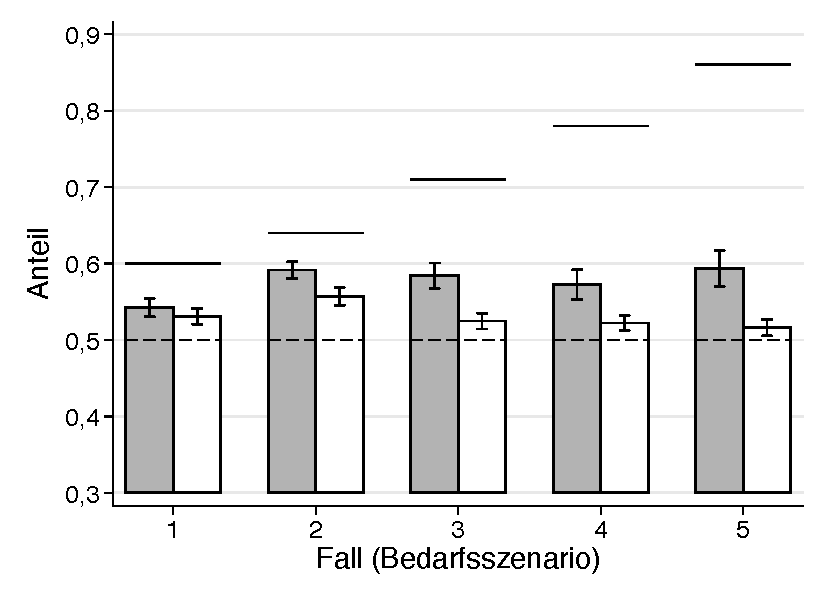
\includegraphics[width=1\linewidth]{figures/figure_7_c.pdf}}\\
      \textcolor{gray}{Anteil Person A Bedarfsszenario}
      \frame{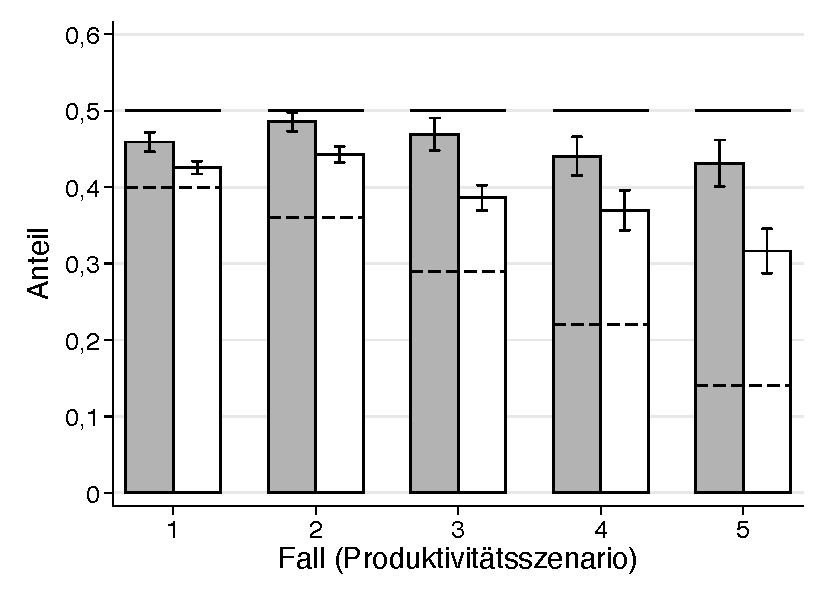
\includegraphics[width=1\linewidth]{figures/figure_7_e.pdf}}\\
      \textcolor{gray}{Anteil Person A Produktivitätsszenario}
   \end{center}
\end{multicols}
\end{frame}


%%%%%%%%%%%%
% FOLIE 72 %
%%%%%%%%%%%%
\begin{frame}{\vspace*{10mm}5\hspace*{1em}Bedarf und Verantwortung}
\begin{center}
   \frame{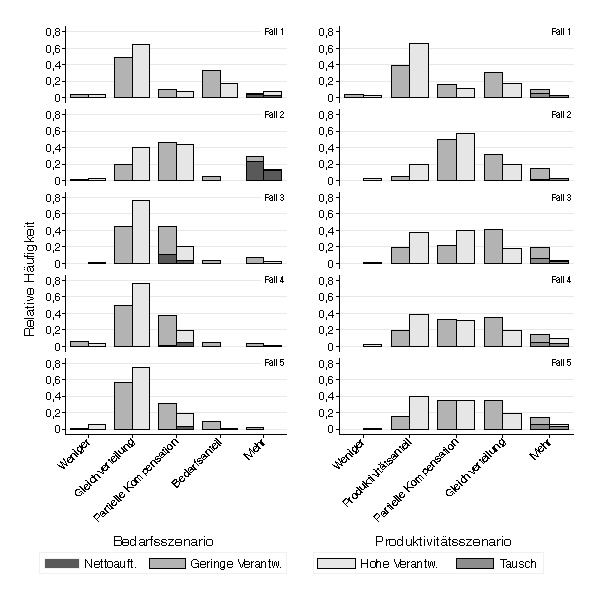
\includegraphics[width=0.45\linewidth]{figures/figure_9.pdf}}\\
   \textcolor{gray}{Verteilungstypen}
\end{center}
\end{frame}


%%%%%%%%%%%%
% FOLIE 73 %
%%%%%%%%%%%%
\begin{frame}{\vspace*{10mm}6.2\hspace*{1em}Studie 2}
\begin{multicols}{2}
   \enquote{Die Person benötigt das Holz, um im Winter gesund zu bleiben und zu überleben. Sie heizt ihre Hütte ausschließlich mit Holz. Je mehr Holzscheite die Person bekommt, desto höher ist die Wahrscheinlichkeit, dass sie gesund bleiben wird. Wenn die Person gar kein Holz bekommt, wird sie mit Sicherheit nicht gesund bleiben. Wenn die Person alles verfügbare Holz bekommt, wird sie mit Sicherheit gesund bleiben.}\\
   \medskip
   \textcolor{gray}{(Ermöglichungsformulierung)}
   \vfill
   \begin{center}
      \frame{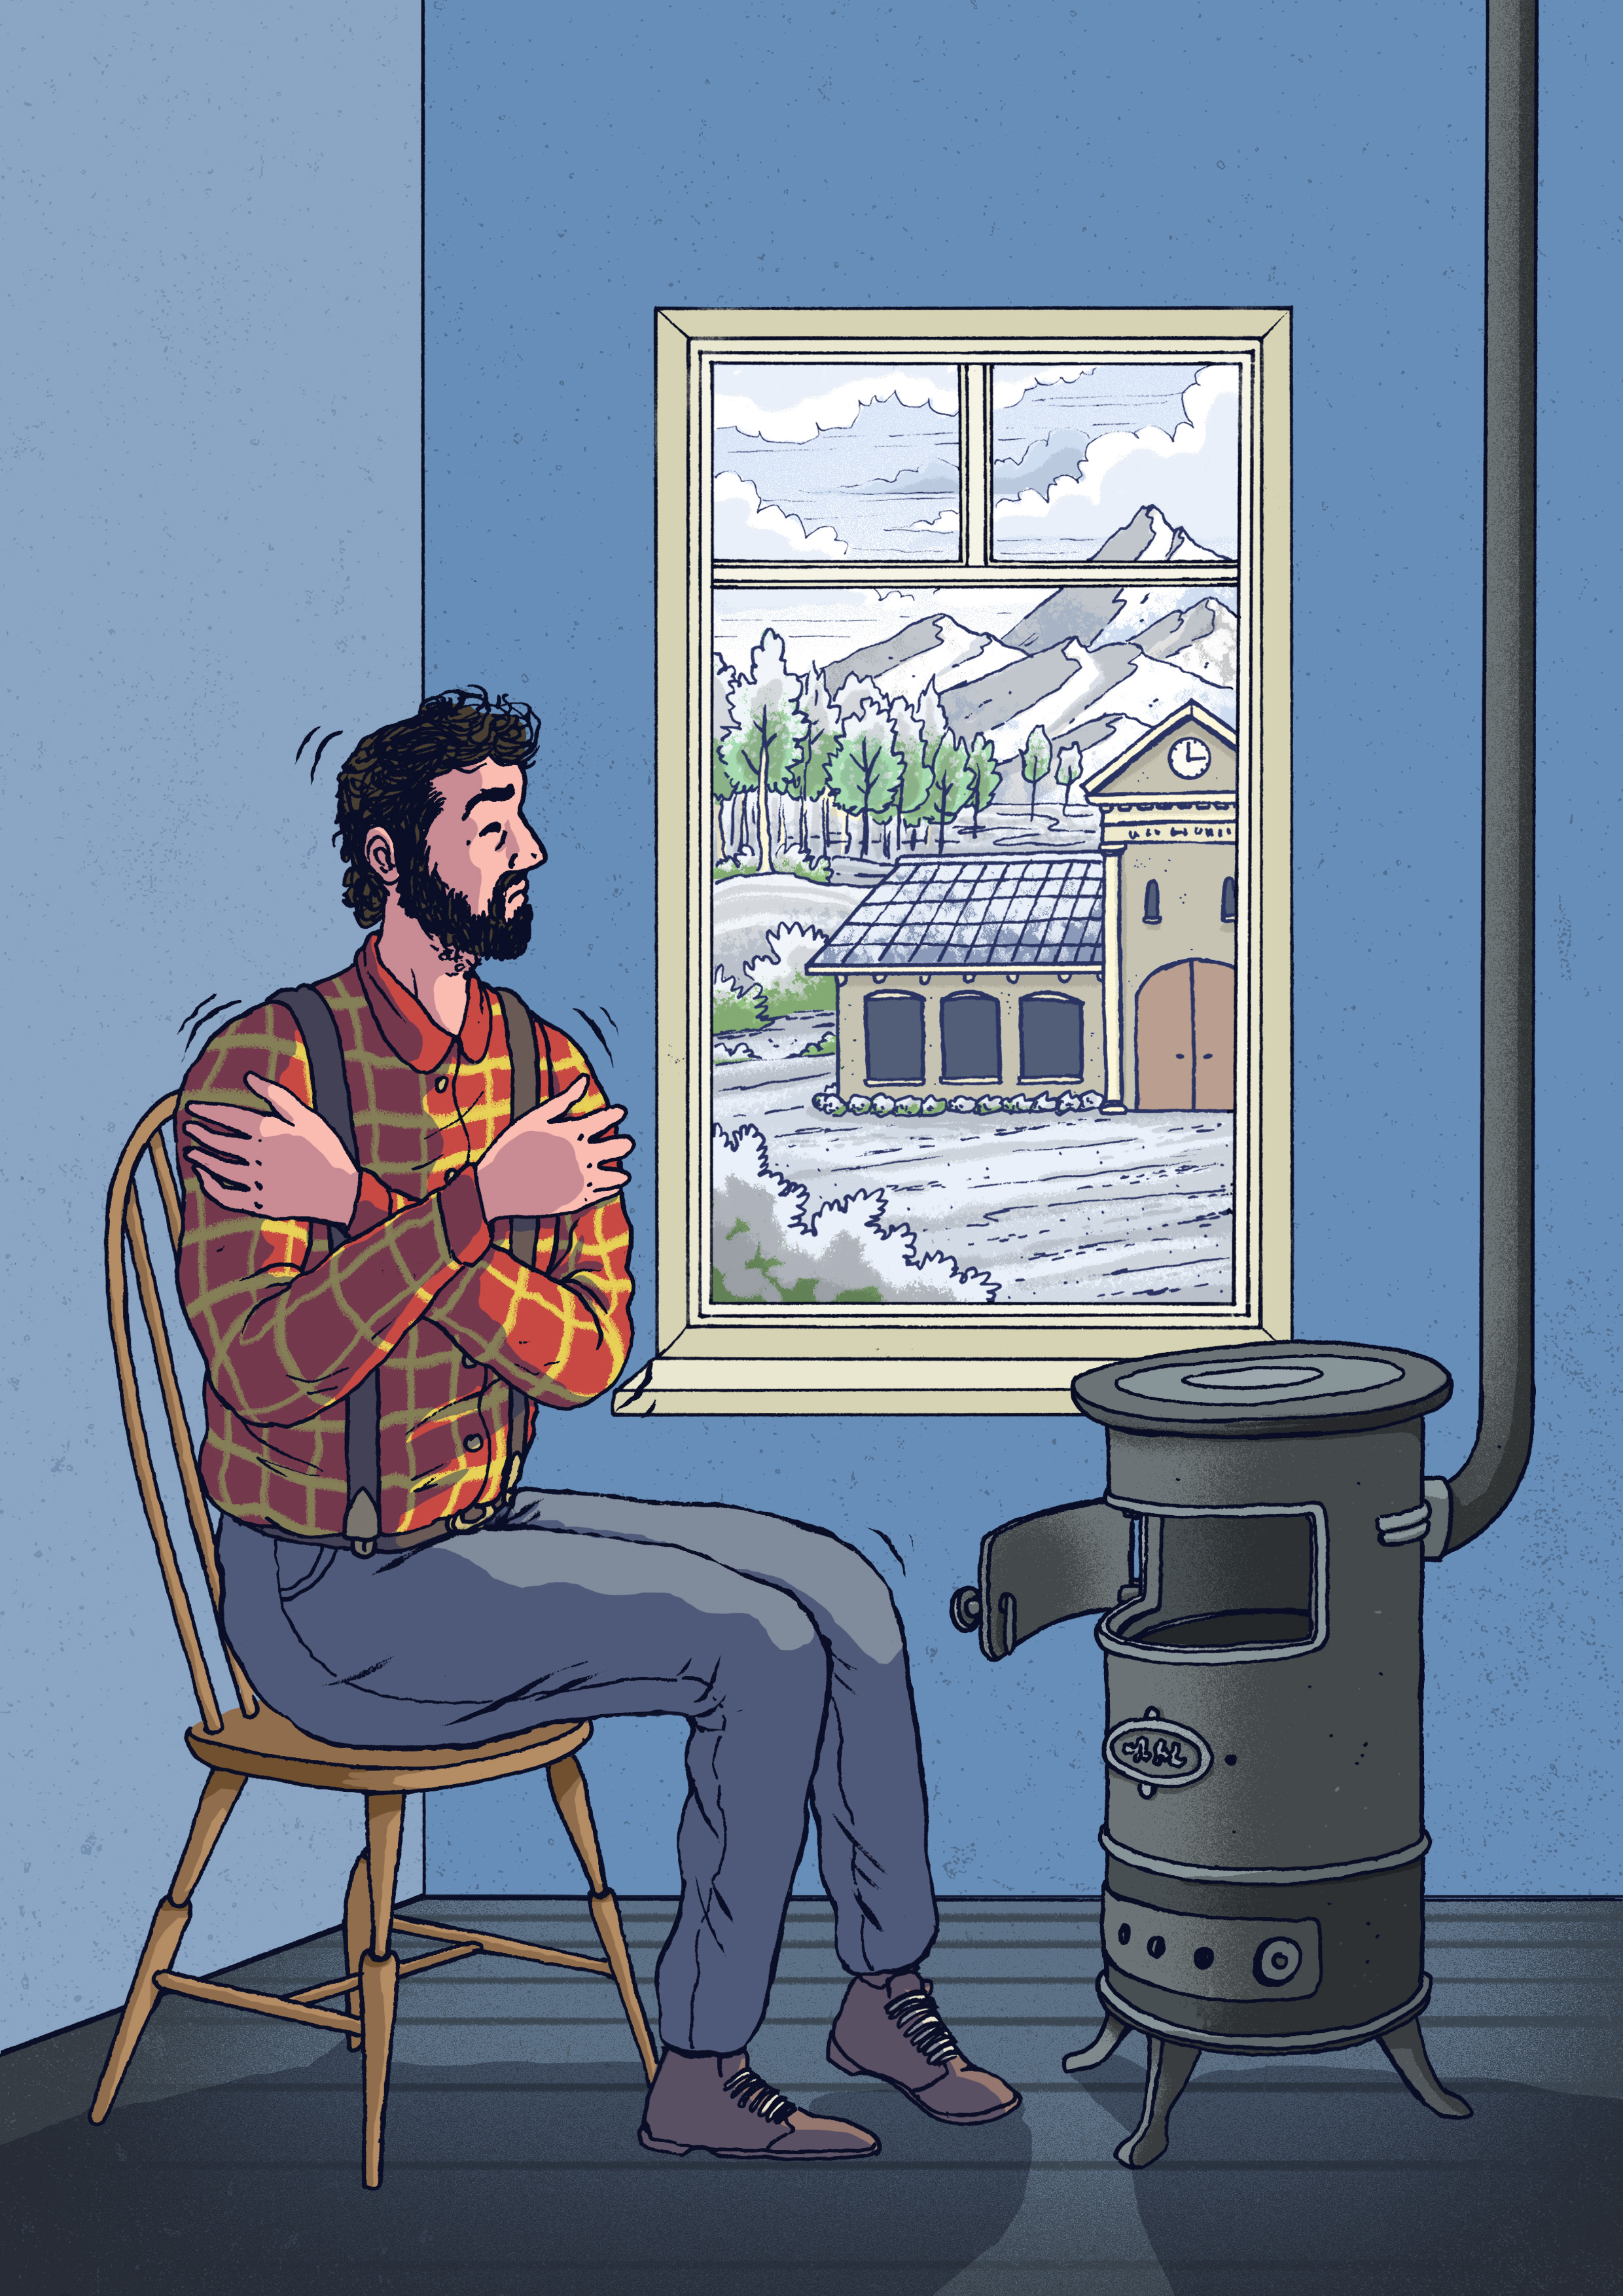
\includegraphics[width=0.6\linewidth]{figures/figure_11.jpg}}\\
      \textcolor{gray}{Illustration \textit{Überleben}}
   \end{center}
\end{multicols}
\end{frame}


%%%%%%%%%%%%
% FOLIE 74 %
%%%%%%%%%%%%
\begin{frame}{\vspace*{10mm}6.2\hspace*{1em}Studie 2}
\begin{multicols}{2}
   \enquote{Die Person benötigt das Holz, um es im Winter warm zu haben. Sie heizt ihre Hütte ausschließlich mit Holz. Je mehr Holzscheite die Person bekommt, desto höher ist die Wahrscheinlichkeit, dass sie es warm haben wird. Wenn die Person gar kein Holz bekommt, wird sie es mit Sicherheit nicht warm haben. Wenn die Person alles verfügbare Holz bekommt, wird sie es mit Sicherheit warm haben.}\\
   \medskip
   \textcolor{gray}{(Ermöglichungsformulierung)}
   \vfill
   \begin{center}
      \frame{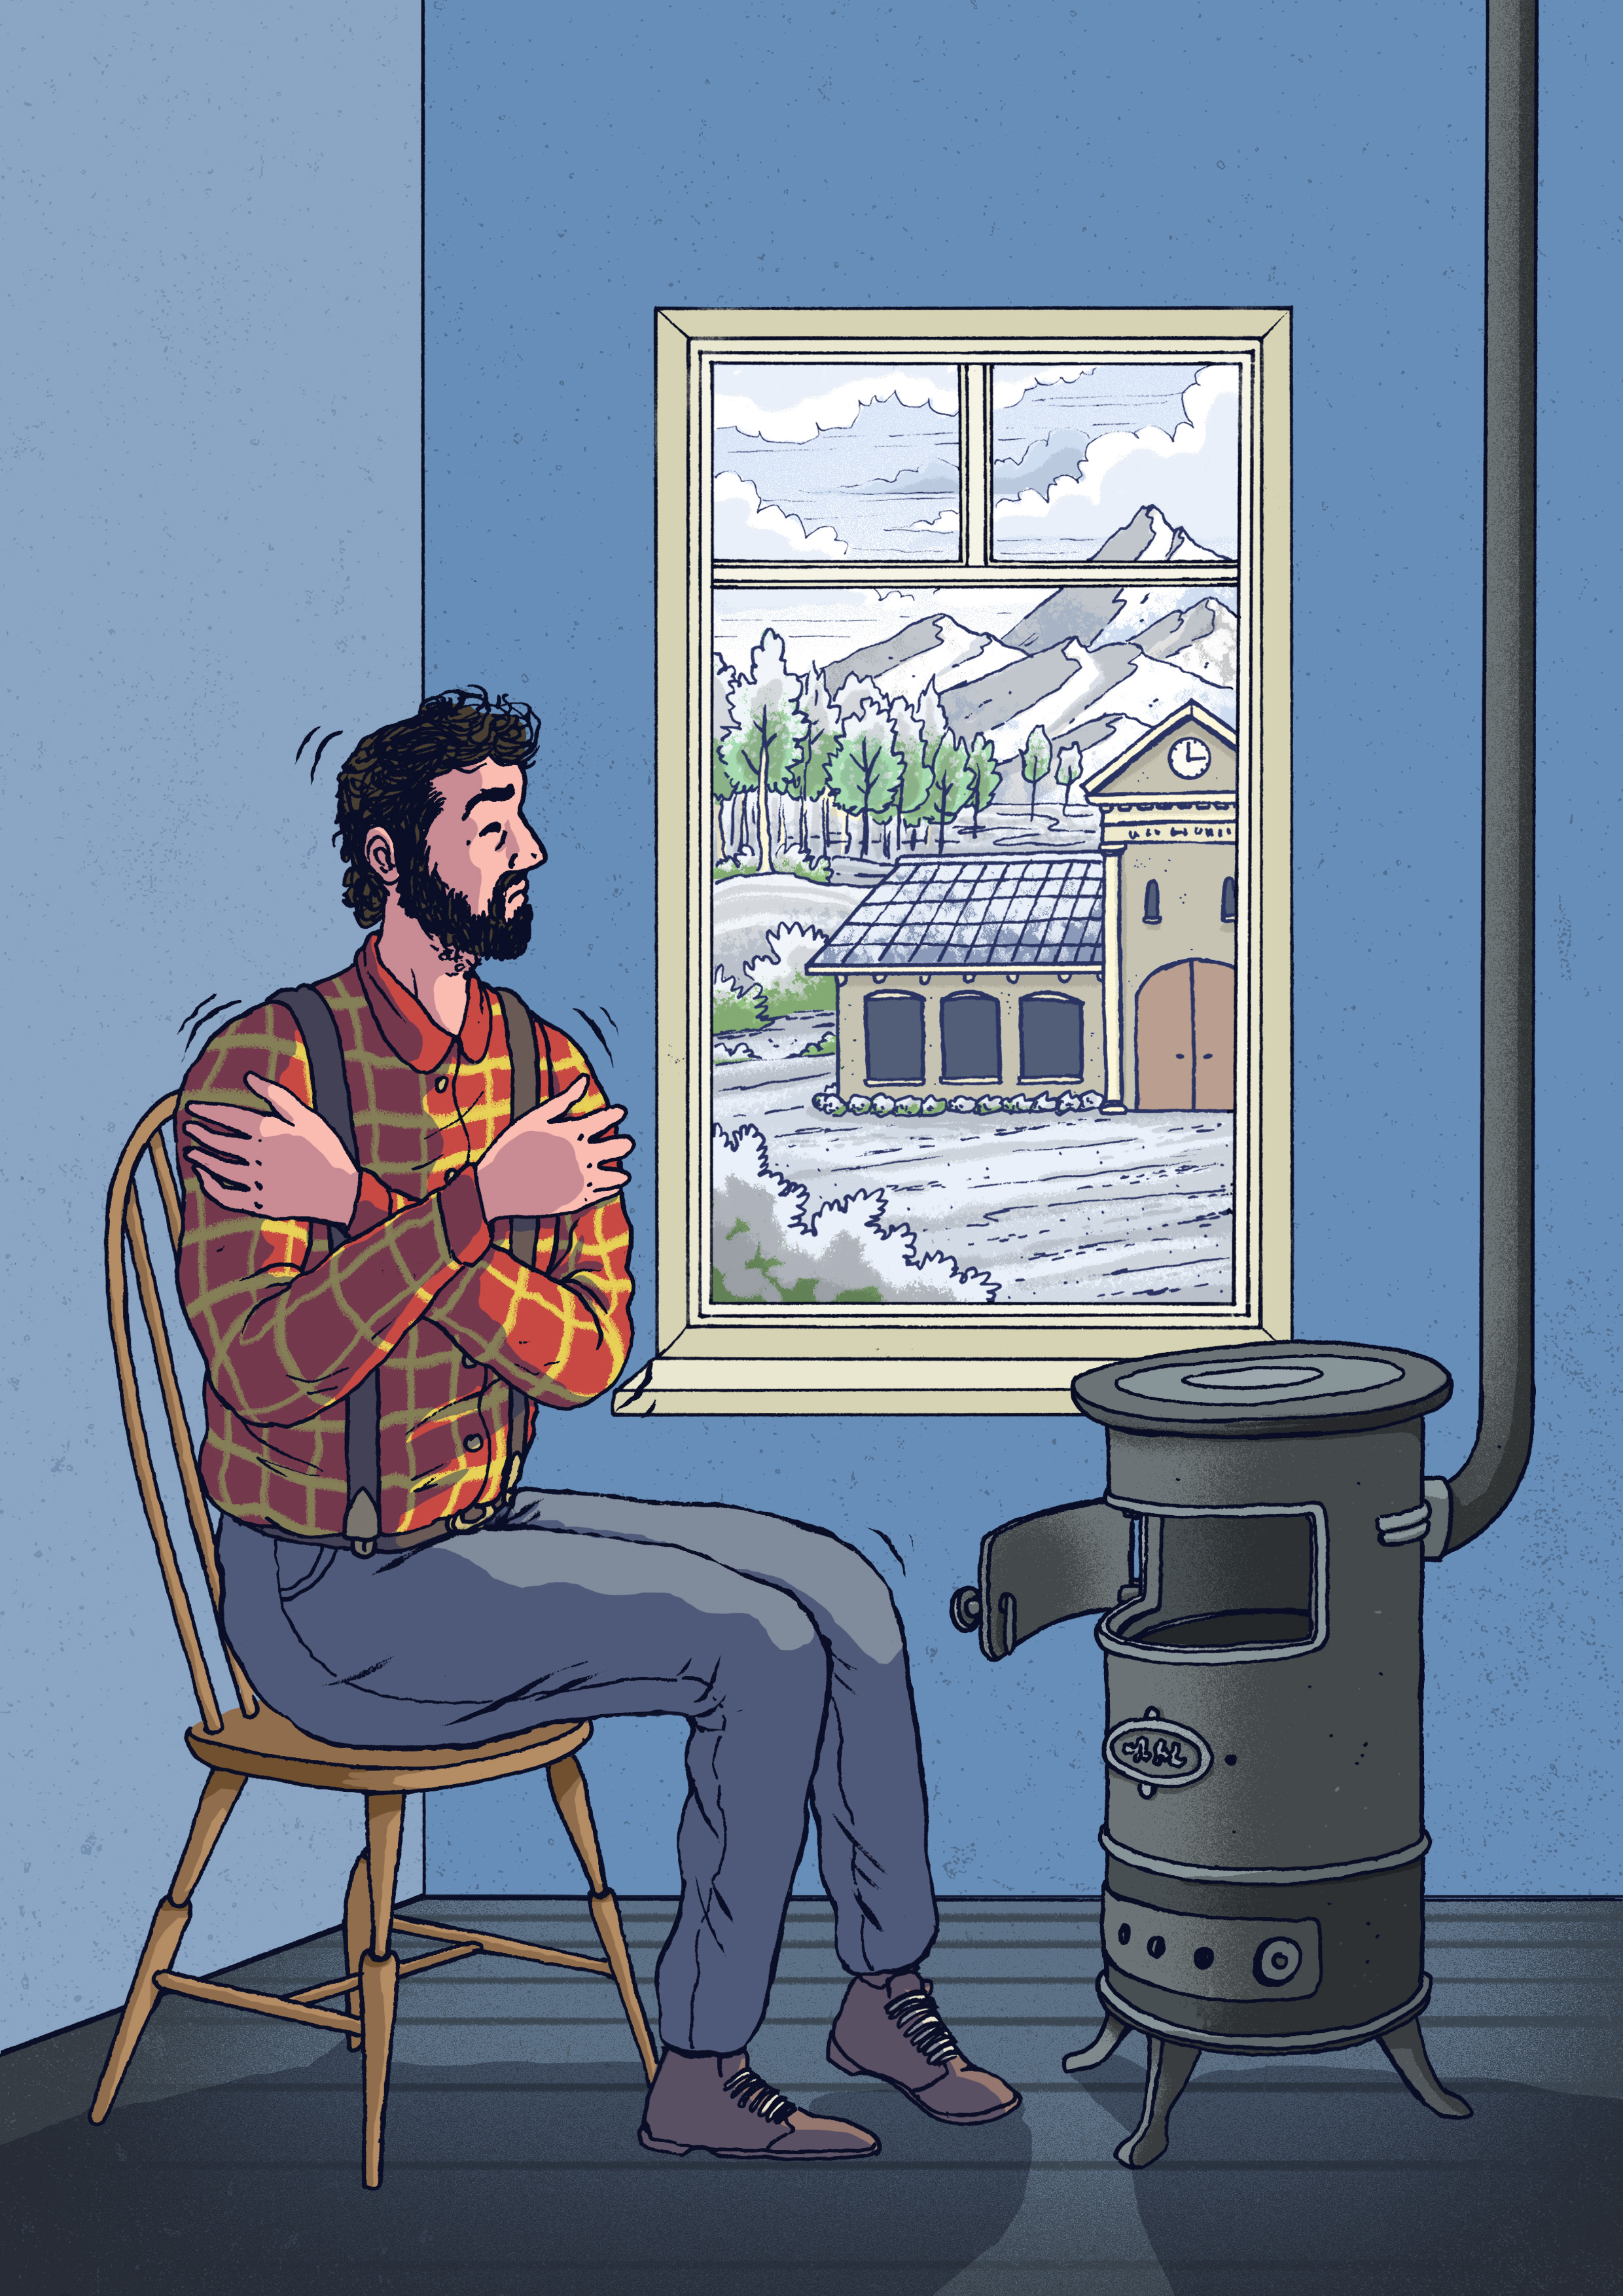
\includegraphics[width=0.6\linewidth]{figures/figure_12.jpg}}\\
      \textcolor{gray}{Illustration \textit{Würde}}
   \end{center}
\end{multicols}
\end{frame}


%%%%%%%%%%%%
% FOLIE 75 %
%%%%%%%%%%%%
\begin{frame}{\vspace*{10mm}6.2\hspace*{1em}Studie 2}
\begin{multicols}{2}
   \enquote{Die Person benötigt das Holz, um im Winter am sozialen Leben teilzuhaben, da es Gang und Gäbe ist, dass man sich im Gemeindehaus trifft und jeder Holz mitbringt, mit dem das Gemeindehaus beheizt werden kann. Je mehr Holzscheite die Person bekommt, desto höher ist die Wahrscheinlichkeit, dass sie am sozialen Leben teilhaben wird. Wenn die Person gar kein Holz bekommt, wird sie mit Sicherheit nicht am sozialen Leben teilhaben. Wenn die Person alles verfügbare Holz bekommt, wird sie mit Sicherheit am sozialen Leben teilhaben.}\\
   \medskip
   \textcolor{gray}{(Ermöglichungsformulierung)}
   \vfill
   \begin{center}
      \frame{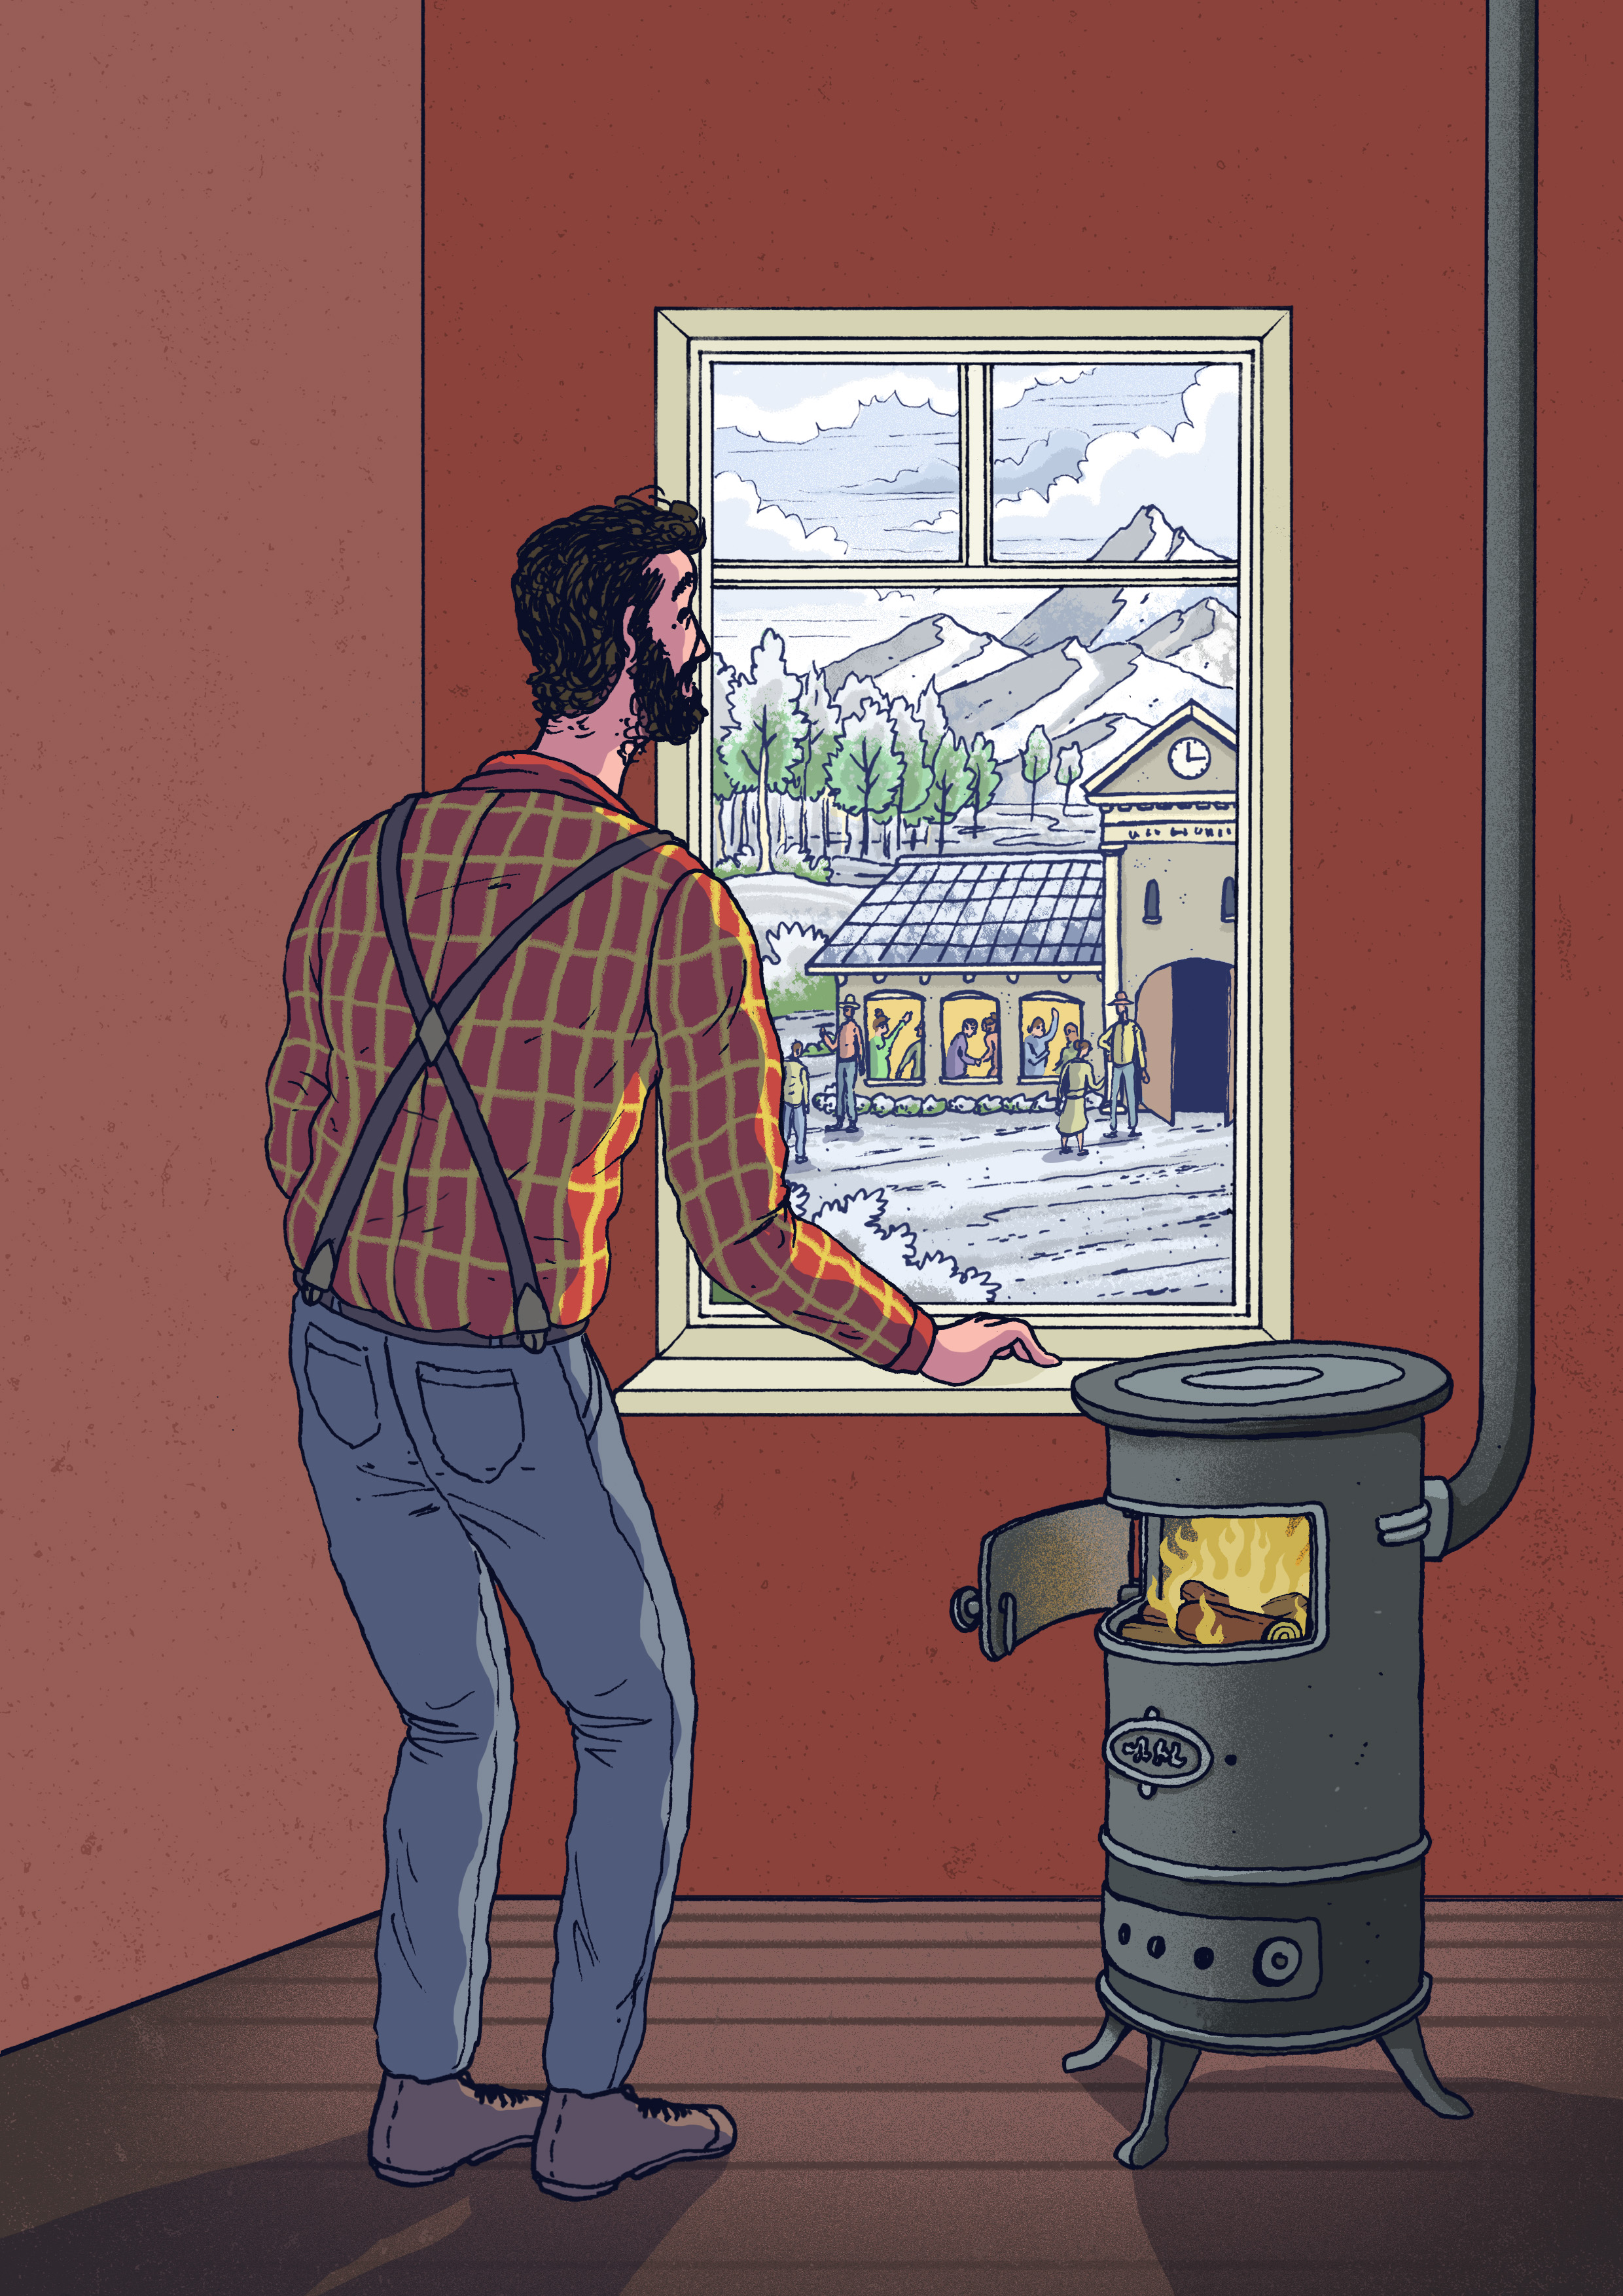
\includegraphics[width=0.6\linewidth]{figures/figure_13.jpg}}\\
      \textcolor{gray}{Illustration \textit{Teilhabe}}
   \end{center}
\end{multicols}
\end{frame}


%%%%%%%%%%%%
% FOLIE 76 %
%%%%%%%%%%%%
\begin{frame}{\vspace*{10mm}6.2\hspace*{1em}Studie 2}
\begin{multicols}{2}
   \enquote{Die Person benötigt das Holz, damit sie ihr Atelier im Winter nutzen kann. Sie heizt ihr Atelier ausschließlich mit Holz. Dort schafft sie in ihrer Freizeit Kunst. Je mehr Holzscheite die Person bekommt, desto höher ist die Wahrscheinlichkeit, dass sie ihr Atelier nutzen wird. Wenn die Person gar kein Holz bekommt, wird sie mit Sicherheit nicht ihr Atelier nutzen. Wenn die Person alles verfügbare Holz bekommt, wird sie mit Sicherheit ihr Atelier nutzen.}\\
   \medskip
   \textcolor{gray}{(Ermöglichungsformulierung)}
   \vfill
   \begin{center}
      \frame{
\includegraphics[width=0.6\linewidth]{figures/figure_14.jpg}}\\
      \textcolor{gray}{Illustration \textit{Autonomie}}
   \end{center}
\end{multicols}
\end{frame}


%%%%%%%%%%%%
% FOLIE 77 %
%%%%%%%%%%%%
\begin{frame}{\vspace*{10mm}6.2\hspace*{1em}Studie 2}
\begin{center}
   \frame{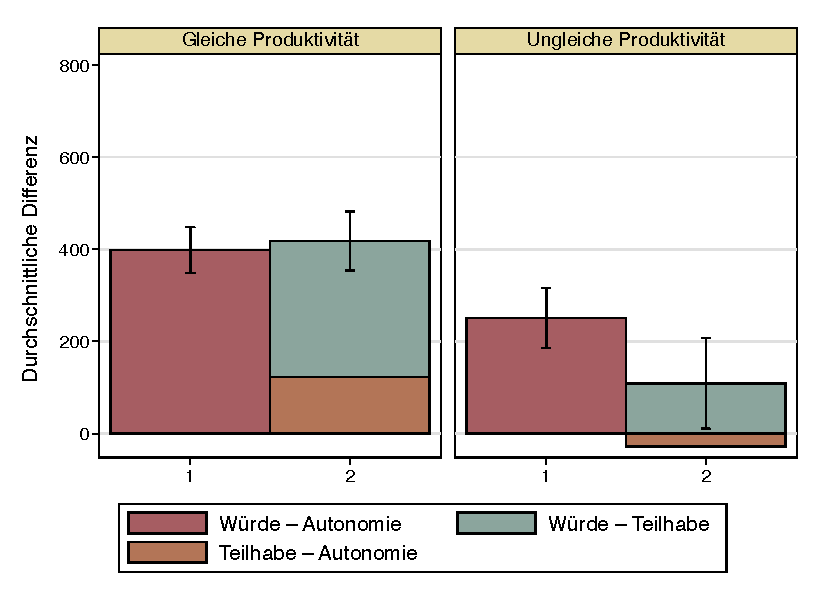
\includegraphics[width=0.5\linewidth]{figures/figure_19.pdf}}\\
   \textcolor{gray}{Additivität \textit{Würde -- Autonomie}}
\end{center}
\end{frame}


%%%%%%%%%%%%
% FOLIE 78 %
%%%%%%%%%%%%
\begin{frame}{\vspace*{10mm}6.2\hspace*{1em}Studie 2}
\begin{center}
   \frame{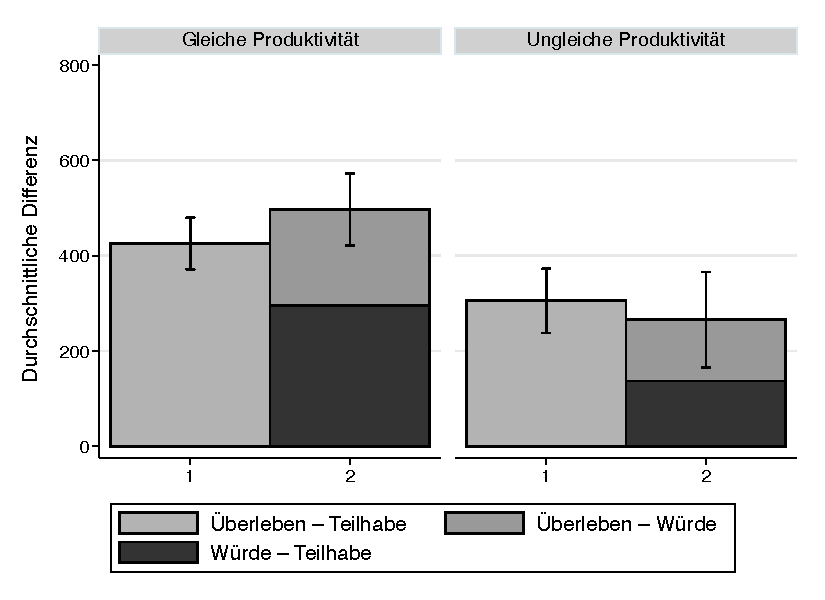
\includegraphics[width=0.5\linewidth]{figures/figure_20.pdf}}\\
   \textcolor{gray}{Additivität \textit{Überleben -- Teilhabe}}
\end{center}
\end{frame}


\end{document}
